\documentclass[10pt]{book}

\usepackage[letterpaper,top=2.5cm,bottom=2.5cm,left=2.5cm,right=2.5cm]{geometry}
\usepackage[T1]{fontenc}
\usepackage[utf8]{inputenc}
\usepackage{graphicx}
\usepackage{multicol}
\usepackage[normalem]{ulem}
\usepackage{float}
\usepackage[usenames,dvipsnames]{color}
\usepackage{amsmath}
\usepackage[table]{xcolor}
\usepackage{xspace}
\usepackage{xhfill}
\usepackage{fancyhdr}
\usepackage[nolist]{acronym}
\usepackage{listings}
% note sure after here
\usepackage{makeidx}
\usepackage{amsmath}
\usepackage[UKenglish]{isodate}
\usepackage{ifthen}
\usepackage{textcomp}
\usepackage{alltt}
\usepackage{ifpdf}
\ifpdf
\usepackage[pdftex,
            pagebackref=true,
            colorlinks=true,
            linkcolor=blue,
            unicode
           ]{hyperref}
\else
\usepackage[ps2pdf,
            pagebackref=true,
            colorlinks=true,
            linkcolor=blue,
            unicode
           ]{hyperref}
\usepackage{pspicture}
\fi
\usepackage{sectsty}
\usepackage{mathptmx}
\usepackage[scaled=.90]{helvet}
\usepackage{courier}
\usepackage[titles]{tocloft}
\usepackage{prettyref}
\usepackage{mdwlist}
\usepackage{enumitem}
\usepackage{framed}
\usepackage{pbox} 
%\usepackage{draftcopy}
%\usepackage{draftwatermark}
\usepackage{wrapfig}
\usepackage{longtable}
\usepackage{caption}
\usepackage{subcaption}


\definecolor{ListingBG}{rgb}{0.91,0.91,0.91}
\definecolor{shadecolor}{rgb}{0.92,0.92,0.92}

\hyphenation{Open-SHMEM}

\renewcommand{\chaptername}{Chapter} 
\renewcommand{\appendixname}{Annex} 

% Place some penalty for doing the break
% The penalty for a ``\gb'' should be greater than a \hyphenpenalty.
% \hyphenpenalty is 50 in plain.tex.
\def\gb{\penalty10000\hskip 0pt plus 8em\penalty4800\hskip 0pt plus-8em%
\penalty10000}

% This macro enables that all "_" (underscore) characters in the pfd
% file are searchable, and that cut&paste will copy the "_" as underscore. 
% Without the following macro, the \_ is treated in searches and cut&paste
% as a " " (space character). 
% This macro does not modify the behavior of _ in math or in verbatim 
% environments. In verbatim environments, the "_" is always treated
% as a searchable character.
%
\DeclareRobustCommand{\_}{\texttt{\char`\_}} 
% 

\def\colorswapnt{\colorlet{saved}{.}\color{ForestGreen}}
\def\colorswapot{\colorlet{saved}{.}\color{red}}
\def\prevcolor{\color{saved}}

\newcommand{\newtext}[1]{\textcolor{ForestGreen}{#1}}
\newcommand{\oldtext}[1]{\textcolor{magenta}{\sout{#1}}}
\newcommand{\insertDocVersion}{1.4}
\newcommand{\openshmem}[1][]{%
  {Open\-SHMEM\ifthenelse{\equal{#1}{}}{}{~#1}}\xspace}
\newcommand{\HEADER}[1]{\textit{#1}}
\newcommand{\FUNC}[1]{\textit{#1}}
\newcommand{\CTYPE}[1]{\textit{#1}}
\newcommand{\VAR}[1]{\textit{#1}}
\newcommand{\CONST}[1]{\textit{#1}}
\newcommand{\const}[1]{\protect\gb\protect{\textsf{\small #1}}\index{CONST:#1}} % Only library_constants.tex table.
\newcommand{\CorCpp}{\textit{C/C++}\xspace}
\newcommand{\CorCppFor}{\textit{C/C++/Fortran}\xspace}
\newcommand{\Fortran}[1][]{%
  \textit{Fortran\ifthenelse{\equal{#1}{}}{}{~#1}}\xspace}
\newcommand{\Cstd}[1][]{%
  \textit{C\ifthenelse{\equal{#1}{}}{}{#1}}\xspace}
\newcommand{\Cpp}[1][]{%
  \textit{C++\ifthenelse{\equal{#1}{}}{}{#1}}\xspace}
\newcommand{\TYPE}{\emph{TYPE}}
\newcommand{\TYPENAME}{\emph{TYPENAME}}
\newcommand{\SIZE}{\emph{SIZE}}

\newcommand{\source}{\textit{source}}
\newcommand{\dest}{\textit{dest}}
\newcommand{\PUT}{\textit{Put}}
\newcommand{\GET}{\textit{Get}}
\newcommand{\OPR}[1]{\textit{#1}}
\newcommand{\barrier}{\FUNC{SHMEM\_BARRIER}\xspace} % why here an not others?
\newcommand{\barrierall}{\FUNC{SHMEM\_BARRIER\_ALL}\xspace} % why here an not others?
\newcommand{\broadcast}{\FUNC{SHMEM\_BROADCAST}}
\newcommand{\collect}{\FUNC{SHMEM\_COLLECT}}
\newcommand{\fcollect}{\FUNC{SHMEM\_FCOLLECT}}
\newcommand{\reduction}{\textit{Reduction Operations}}
\newcommand{\alltoall}{\FUNC{SHMEM\_ALLTOALL}}
\newcommand{\alltoalls}{\FUNC{SHMEM\_ALLTOALLS}}
\newcommand{\shmemprefix}{\textit{SHMEM\_}}
\newcommand{\shmemprefixLC}{\textit{shmem\_}}
\newcommand{\shmemprefixC}{\textit{\_SHMEM\_}}
\newcommand{\ith}{${\textit{i}^{\text{\tiny th}}}$}
\newcommand{\jth}{${\textit{j}^{\text{\tiny th}}}$}
\newcommand{\kth}{${\textit{k}^{\text{\tiny th}}}$}
\newcommand{\lth}{${\textit{l}^{\text{\tiny th}}}$}

\begin{acronym}
\acro{RMA}{\emph{Remote Memory Access}}
\acro{RMO}{\emph{Remote Memory Operation}}
\acro{AMO}{\emph{Atomic Memory Operation}}
\acro{PE}{\emph{Processing Element}}
\acrodefplural{PE}[PEs]{\emph{Processing Elements}}
\acro{PGAS}{\emph{Partitioned Global Address Space}}
\acro{API}{\emph{Application Programming Interface}}
\acro{MPI}{\emph{Message Passing Interface}}
\acro{SPMD}{\emph{Single Program Multiple Data}}
\acro{ARL}{Army Research Laboratory}
\acro{AMD}{Advanced Micro Devices}
\acro{UH}{University of Houston}
\acro{UO}{University of Oregon}
\acro{ORNL}{Oak Ridge National Laboratory}
\acro{LANL}{Los Alamos National Laboratory}
\acro{ESSC}{Extreme Scale Systems Center}
\acro{OSSS}{Open Software System Solutions}
\acro{DoD}{U.S. Department of Defense}
\acro{SBU}{Stonybrook University}
\acro{UTK}{University of Tenneesee at Knoxville}
\acro{HPE}{Hewlett Packard Enterprise}
\end{acronym}


%
% This is used to put line numbers on plain pages.  Used in draft.tex
%
\makeatletter

\def\withlinenumbers{\relax
  \def\@evenfoot{\hbox to 0pt{\hss\LineNumberRuler\hskip 1.5pc}\hfil}\relax
  \def\@oddfoot{\hfil\hbox to 0pt{\hskip 1.5pc\LineNumberRuler\hss}}}

\def\LineNumberRuler{\vbox to 0pt{\vss\normalsize \baselineskip13.6pt
    \lineskip 1pt \normallineskip 1pt \def\baselinestretch{1}\relax
    \LNR{1}\LNR{2}\LNR{3}\LNR{4}\LNR{5}\LNR{6}\LNR{7}\LNR{8}\LNR{9}
    \LNR{10}\LNR{11}\LNR{12}\LNR{13}\LNR{14}
        \LNR{15}\LNR{16}\LNR{17}\LNR{18}\LNR{19}
    \LNR{20}\LNR{21}\LNR{22}\LNR{23}\LNR{24}
        \LNR{25}\LNR{26}\LNR{27}\LNR{28}\LNR{29}
    \LNR{30}\LNR{31}\LNR{32}\LNR{33}\LNR{34}\LNR{35}
        \LNR{36}\LNR{37}\LNR{38}\LNR{39}
    \LNR{40}\LNR{41}\LNR{42}\LNR{43}\LNR{44}
        \LNR{45}\LNR{46}\LNR{47}\LNR{48}
    \vskip 31pt}}
\def\LNR#1{\hbox to 1pc{\hfil\tiny#1\hfil}}

\def\ps@plainwithlinenumbers{\let\@mkboth\@gobbletwo
     \def\@oddhead{}
     \def\@oddfoot{\hfil\rm\thepage\hfil
       \hbox to 0pt{\hskip 1.5pc\LineNumberRuler\hss}}
     \def\@evenhead{}
     \def\@evenfoot{\hbox to 0pt{\hss
     \LineNumberRuler\hskip 1.5pc}\rm\hfil\thepage\hfil}}

    % Contents is done with \chapter*{Contents}, so we need to turn off the
    % line numbers in this case.  Easiest to look at def

\newwrite\chappages
\immediate\openout\chappages=chappage.txt
\def\writespace{ }

\def\incontents{0}
\newif\ifcontents
\contentsfalse
\def\chapter{\clearpage \ifcontents\else\thispagestyle{plainwithlinenumbers}\fi
        \write\chappages{Chapter \thechapter\writespace - \the\count0}
        \global\@topnum\z@ \@afterindentfalse \secdef\@chapter\@schapter}

\makeatother

%
% End this is used to put line numbers on plain pages.  Used in draft.tex
%

%
% Use Sans Serif font for sections, etc.
%
\makeatletter
\def\section{\@startsection {section}{1}{\z@}{-3.5ex plus -1ex minus 
-.2ex}{2.3ex plus .2ex}{\Large\sf}}
\def\subsection{\@startsection{subsection}{2}{\z@}{-3.25ex plus -1ex minus 
-.2ex}{1.5ex plus .2ex}{\large\sf}}
\def\subsubsection{\@startsection{subsubsection}{3}{\z@}{-3.25ex plus 
-1ex minus -.2ex}{1.5ex plus .2ex}{\normalsize\sf\bf}}
\def\paragraph{\@startsection {paragraph}{4}{\z@}{3.25ex plus 1ex 
minus .2ex}{-1em}{\normalsize\sf}}
\makeatother
%
% End use Sans Serif font for sections, etc.  S. Otto
%


%
% This section is for example code listings
%
\definecolor{gray}{rgb}{0.92,0.92,0.92}

\lstset{ % set defaults for languages not otherwise defined
  breakatwhitespace=false,         % sets if automatic breaks should only happen at whitespace
  basicstyle=\ttfamily\footnotesize,
  breaklines=true,                 % sets automatic line breaking
  escapeinside={|}{|},          % if you want to add LaTeX within your code
  extendedchars=true,              % lets you use non-ASCII characters; for 8-bits 
                                   % encodings only, does not work with UTF-8
  keepspaces=true,                 % keeps spaces in text, useful for keeping indentation of code 
                                   % (possibly needs columns=flexible)
  morekeywords={*,...},            % if you want to add more keywords to the set
  showspaces=false,                % show spaces everywhere adding particular underscores; 
                                   % it overrides 'showstringspaces'
  showstringspaces=false,          % underline spaces within strings only
  showtabs=false,                  % show tabs within strings adding particular underscores
}

\def\StandardListing {
  \lstset {
    breakatwhitespace=false,         % sets if automatic breaks should only happen at whitespace
    basicstyle=\ttfamily\footnotesize,
    breaklines=true,                 % sets automatic line breaking
    escapeinside={\%*}{*)},          % if you want to add LaTeX within your code
    extendedchars=true,              % lets you use non-ASCII characters; for 8-bits 
                                     % encodings only, does not work with UTF-8
    keepspaces=true,                 % keeps spaces in text, useful for keeping
                                     % indentation of code (possibly needs columns=flexible)
    morekeywords={*,...},            % if you want to add more keywords to the set
    showspaces=false,                % show spaces everywhere adding particular underscores; 
                                     % it overrides 'showstringspaces'
    showstringspaces=false,          % underline spaces within strings only
    showtabs=false,                  % show tabs within strings adding particular underscores
    backgroundcolor=\color{gray}, 
  }
}

\def\ProgramNumberedListing {
  \StandardListing
  \lstset {
    numbers=left,
    numberstyle=\footnotesize
  }
}

\newcommand{\numberedlisting}[2] {
  \ProgramNumberedListing
  \lstinputlisting[#1]{#2}
  \StandardListing
}

\newcommand{\outputlisting}[2] {
\begin{minipage}{\linewidth}
\vspace{0.1in}
  \lstinputlisting[#1]{#2}
  \StandardListing
\vspace{0.1in}
\end{minipage}
}

\lstdefinelanguage{OSH+C}[]{C}{
  classoffset=1,
  morekeywords={
    size_t, ptrdiff_t,
    SHMEM_BCAST_SYNC_SIZE, SHMEM_SYNC_VALUE,
    start_pes,
    my_pe, _my_pe, shmem_my_pe,
    num_pes, _num_pes, shmem_n_pes,
    shmem_int_p, shmem_short_p, shmem_long_p,
    shmem_int_put, shmem_short_put, shmem_long_put,
    shmem_barrier_all, shmem_barrier,
    shmalloc,  shfree, shrealloc,
    shmem_broadcast32, shmem_broadcast64,
    shmem_short_inc, shmem_int_inc, shmem_long_inc,
    shmem_short_add, shmem_int_add, shmem_long_add,
    shmem_short_finc, shmem_int_finc, shmem_long_finc,
    shmem_short_fadd, shmem_int_fadd, shmem_long_fadd,
    shmem_set_lock, shmem_test_lock, shmem_clear_lock,
    shmem_long_sum_to_all,
    shmem_complexd_sum_to_all,
    shmem_cmp_t
  },
  keywordstyle=\color{black}\textbf,
  classoffset=0,
  sensitive=true
}

\lstdefinelanguage{OSH2+C}[]{OSH+C}{
  classoffset=1,
  morekeywords={
    shmem_init,
    shmem_finalize,
    shmem_malloc,
    shmem_my_pe,
    shmem_error,
    shmem_global_exit,
  },
  keywordstyle=\color{black}\textbf,
  classoffset=0,
  sensitive=true
}

\lstdefinelanguage{OSH+F}[]{Fortran}{
  classoffset=1,
  morekeywords={
    SHMEM_BCAST_SYNC_SIZE, SHMEM_SYNC_VALUE,
    start_pes,
    my_pe, shmem_my_pe,
    num_pes, shmem_n_pes,
    shmem_int_p, shmem_short_p, shmem_long_p,
    shmem_int_put, shmem_short_put, shmem_long_put,
    shmem_barrier_all, shmem_barrier,
    shpalloc,  shpdeallc, shpclmove,
    shmem_broadcast32, shmem_broadcast64,
    shmem_broadcast4, shmem_broadcast8,
    shmem_short_inc, shmem_int_inc, shmem_long_inc,
    shmem_short_add, shmem_int_add, shmem_long_add,
    shmem_short_finc, shmem_int_finc, shmem_long_finc,
    shmem_short_fadd, shmem_int_fadd, shmem_long_fadd,
    shmem_set_lock, shmem_test_lock, shmem_clear_lock,
    shmem_long_sum_to_all,
  },
  keywordstyle=\color{black}\textbf,
  classoffset=0,
  sensitive=false
}

\lstdefinelanguage{OSH2+F}[]{OSH+F}{
  classoffset=1,
  morekeywords={
    shmem_init,
    shmem_finalize,
    shmem_malloc,
    shmem_my_pe,
    shmem_error,
    shmem_global_exit,
  },
  keywordstyle=\color{black}\textbf,
  classoffset=0,
  sensitive=true
}

%
% End this section is for example code listings
%

%
% Deprecation Helpers
%

\newcommand{\strikeline}[1][red]{{\color{#1}\raisebox{.5ex}{\rule{1em}{.4pt}}}}
\newcommand{\stretchline}[1][red]{\xrfill[.5ex]{.4pt}[#1]}
\newcommand{\DeprecationStart}[1][red]{{\color{#1} deprecation start} \mbox{}}
\newcommand{\DeprecationEnd}[1][red]{{\color{#1} deprecation end} \mbox{}}

\newcommand{\StartDeprecateBlock}{
  {\strikeline\mbox{} \DeprecationStart \stretchline\mbox{}}}
\newcommand{\EndDeprecateBlock}{%
  \mbox{}\stretchline\mbox{} \DeprecationEnd \strikeline}

\newenvironment{DeprecateBlock}{%
  \par \StartDeprecateBlock \par}{\par \EndDeprecateBlock \par}

\newcommand{\StartInlineDeprecate}{%
  \strikeline\mbox{} \DeprecationStart \strikeline \mbox{}}
\newcommand{\EndInlineDeprecate}{%
  \strikeline\mbox{} \DeprecationEnd \strikeline}
\newenvironment{DeprecateInline}{\StartInlineDeprecate}{\EndInlineDeprecate}

%
% Library API description template commands
%

\newcommand{\deprecationstart}{\color{red} \raisebox{.5ex}{\rule{1em}{.4pt}}
  deprecation start \xrfill[.5ex]{.4pt}[red] \mbox{}}
\newcommand{\deprecationend}{\mbox{}\xrfill[.5ex]{.4pt}[red]\mbox{} \color{red}
  deprecation end \raisebox{.5ex}{\rule{1em}{.4pt}}}

\newenvironment{deprecate}{\deprecationstart \\}{\\ \deprecationend}

\newcommand{\apisummary}[1]{
    #1
\hfill
}

\newenvironment{apidefinition}{
\begin{description}
\item[SYNOPSIS] \hfill \\ \\ 
\vspace{-2em}
}
{
\end{description}
}

\lstnewenvironment{Cpp11synopsis}
{
  \textbf{C++11:}
  \lstset{language={C++}, backgroundcolor=\color{gray}, lineskip=2pt,
  morekeywords={size_t, TYPE, noreturn}, aboveskip=0pt, belowskip=0pt}}{}

\lstnewenvironment{C11synopsis}
{ 
  \textbf{C11:} 
  \lstset{language={C}, backgroundcolor=\color{gray}, lineskip=2pt,
  morekeywords={size_t, ptrdiff_t, TYPE, _Noreturn, shmem_cmp_t},
  aboveskip=0pt, belowskip=0pt}}{}

\lstnewenvironment{CsynopsisCol}
{ 
  \lstset{language={C}, backgroundcolor=\color{gray}, lineskip=2pt,
  morekeywords={size_t, ptrdiff_t, TYPE, TYPENAME, SIZE, shmem_cmp_t},
  aboveskip=0pt, belowskip=0pt}}{}


\lstnewenvironment{Csynopsis}
{ 
  \textbf{C/C++:} 
  \lstset{language={C}, backgroundcolor=\color{gray}, lineskip=2pt,
  morekeywords={size_t, ptrdiff_t, TYPE, TYPENAME, SIZE, shmem_cmp_t},
  aboveskip=0pt, belowskip=0pt}}{}

\lstnewenvironment{CsynopsisST}
{ 
  \textbf{C/C++:} 
  \color{red}  
  {\lstset{language={C}, backgroundcolor=\color{gray}, lineskip=2pt,
  morekeywords={size_t}, aboveskip=0pt, belowskip=0pt}}
  }
  {}
  
\lstnewenvironment{Fsynopsis}
{ \deprecationstart \\
  \textbf{FORTRAN:}
  \lstset{language={Fortran}, backgroundcolor=\color{gray}, lineskip=3pt,
  deletekeywords=[2]{STATUS},
  deletekeywords=[3]{LOG}, aboveskip=0pt,
  belowskip=0pt}}
{ \deprecationend }

\newenvironment{apiarguments}{
\newcommand{\apiargument}[3]{
\begin{tabular}{p{2cm} p{2cm} p{10cm}}
\textbf{##1} & \textit{##2} & {##3} \\ 
\end{tabular}
}
\hfill
\item[DESCRIPTION] \hfill 

\begin{description}
\item[Arguments] \hfill \\
}
{
\hfill
\end{description}
}

\newcommand{\apidescription}[1]{
\begin{description}
\vspace{-1em}
\item[API description] \hfill \\ 
    #1
\hfill
}

\newcommand{\apidesctable}[4] {\hfill \\ #1 \\ \\
    \begin{tabular}{p{5cm} p{9cm}}
       \hline
       #2 & #3 \\
       \hline \tabularnewline
       \end{tabular}\\
        #4
}  

\newcommand{\apireturnvalues}[1]{
\hfill 
\item[Return Values] \hfill \\
    #1
\\
\hfill
}

\newcommand{\apitablerow}[2]{
 \begin{tabular}{p{5cm} p{9cm}}
 #1 & #2 \tabularnewline
  \end{tabular}\\
}

\newcommand{\apinotes}[1]{
\item[Notes] \hfill \\
    #1
\hfill \\
\end{description}
}

\newcommand{\apiimpnotes}[1]{
\begin{description}
\item[Note to implementors] \hfill \\
    #1
\hfill \\
\end{description}
}

\newenvironment{apiexamples}{
\newcommand{\apicexample}[3]{
    ##1
    \lstinputlisting[language={C}, tabsize=2,
      basicstyle=\ttfamily\footnotesize,
      morekeywords={size_t, ptrdiff_t, shmem_cmp_t}]{##2}
    ##3 }
\newcommand{\apifexample}[3]{
    ##1
    \lstinputlisting[language={Fortran}, tabsize=2,
    basicstyle=\ttfamily\footnotesize, deletekeywords={TARGET}]{##2}
    ##3 }
\vspace{-2pt}
\item[EXAMPLES] \hfill \\
\vspace{-2pt}
}
{
}

%
% End library API description template commands
%


\makeindex

\begin{document}

\hypersetup{pageanchor=true,citecolor=blue}

% Set header/footer for opening content
\pagestyle{fancy}
\fancyhead{}
\fancyhead[LE,LO]{\insertDocVersion}
\fancyhead[CO,CE]{--- DRAFT ---}
\SetWatermarkText{DRAFT}
\SetWatermarkScale{1}
\SetWatermarkLightness{.91}
\fancyfoot[CE,CO]{\thepage} %affects page numbering for the first pages, 
                            %except the first ToC page

\pagenumbering{roman} %sets coverpage and toc page numbers to roman numerals

\thispagestyle{empty}
\begin{center}
\textbf{\Huge \openshmem}
\par
\end{center}

\begin{center}
\textbf{\LARGE Application Programming Interface}\\
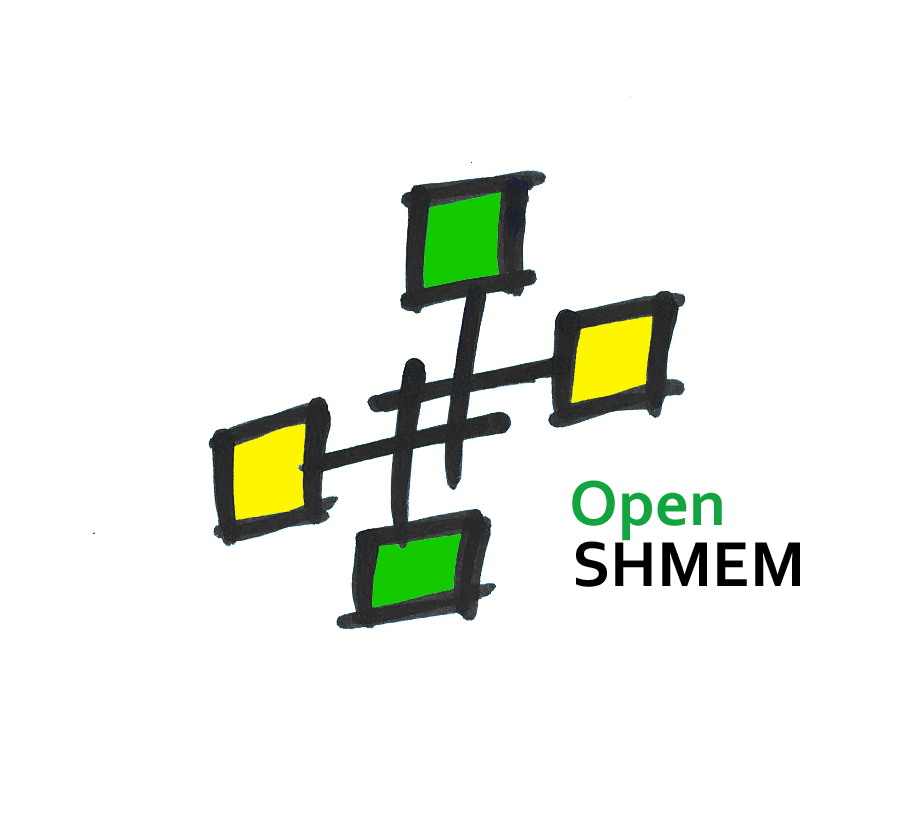
\includegraphics[scale=0.65]{figures/OpenSHMEM_Pound}\\
\url{http://www.openshmem.org/}
\par
\end{center}

\begin{center}
Version \insertDocVersion
\par
\end{center}

\vspace{0.5in}
\begin{center}
\today
\end{center}

\vspace{0.5in}

\vfill{}

\section*{Developed by}
\begin{itemize}
\item High Performance Computing Tools group at the University of Houston\\
  \url{http://www.cs.uh.edu/~hpctools/} 
\item Extreme Scale Systems Center, Oak Ridge National Laboratory\\
  \url{http://www.csm.ornl.gov/essc/} 
\end{itemize}
\pagebreak{}

\section*{Sponsored by}
\begin{itemize}
\item \ac{DoD}\\
  \url{http://www.defense.gov/ }
\item \ac{ORNL}\\
  \url{http://www.ornl.gov/} 
\end{itemize}

\section*{Authors and Collaborators}
\begin{itemize}
\item Monika ten Bruggencate
\item Matthew Baker, \ac{ORNL}
\item Barbara Chapman, \ac{UH} 
\item Tony Curtis, \ac{UH}
\item Eduardo D'Azevedo, \ac{ORNL}
\item James Dinan, Intel
\item Karl Feind, SGI
\item Manjunath Gorentla Venkata, \ac{ORNL}
\item Jeff Hammond, Intel
\item Oscar Hernandez, \ac{ORNL}
\item David Knaak, Cray Inc.
\item Gregory Koenig, \ac{ORNL}
\item Jeff Kuehn, \ac{LANL}
\item Graham Lopez, \ac{ORNL}
\item Jens Manser, \ac{DoD}
\item Tiffany M. Mintz, \ac{ORNL}
\item Nicholas Park, \ac{DoD}
\item Steve Poole, OSSS
\item Wendy Poole, OSSS
\item Swaroop Pophale, \ac{ORNL}
\item Michael Raymond, SGI
\item Pavel Shamis, \ac{ORNL}
\item Sameer Shende, \ac{UO}
\item Lauren Smith, \ac{DoD}
\item Aaron Welch, \ac{ORNL}

\end{itemize}

\date{\today}

\section*{Acknowledgements}
The \openshmem specification belongs to Open Source Software Solutions, Inc.
(OSSS), a non-profit organization, under an agreement with SGI. The development
work of the specification is supported by the Oak Ridge National Laboratory
Extreme Scale Systems Center and the Department of Defense.\\
\\
We would also like to acknowledge the contribution of the members of the
\openshmem mailing list for their ideas, discussions, suggestions, and
constructive criticism which has helped us improve this document.




\setcounter{tocdepth}{4}
\setcounter{secnumdepth}{4}
\tableofcontents

\mainmatter  % included for use of documenttype 'book' 

% Set header/footer for main content
\pagestyle{fancy}   %replacing {headings} with {fancy} for customization 
\fancyhf{}
\fancyhead[RE, LO]{\rightmark}
\fancyhead[RO, LE]{\thepage}
\renewcommand{\headrulewidth}{0pt}
\let\thesectionOrig\thesection % Used by backmatter to restore Annex numbering.
\renewcommand{\thesection}{\arabic{section}}

{ %using setlength to force standardized spacing, if needed
% this command is ended in backmatter.tex
%\setlength{\baselineskip}{3pt plus 3pt minus 3pt}

\setlength{\parskip}{3pt}




\section{The \openshmem Effort}\label{subsec:openshmem_effort}
\openshmem is a \ac{PGAS} library interface specification. \openshmem aims to
provide a standard \ac{API} for SHMEM libraries to aid portability and
facilitate uniform predictable results of \openshmem programs by explicitly
stating the behavior and semantics of the \openshmem library calls. Through the
different versions, \openshmem will continue to address the requirements of the
\ac{PGAS} community.  As of this specification, many existing vendors support
\openshmem-compliant implementations and new vendors are developing
\openshmem library implementations to help the users write portable \openshmem
code. This ensures that programs can run on multiple platforms without having to
deal with subtle vendor-specific implementation differences. For more details on
the history of \openshmem please refer to the
\hyperref[sec:openshmem_history]{History of \openshmem} section.  

The \openshmem\footnote{The \openshmem specification is owned by Open Source
Software Solutions Inc., a non-profit organization, under an agreement with
SGI.}  effort is driven by the \ac{ESSC} at \ac{ORNL} and the University of
Houston with significant input from the \openshmem community. Besides the
specification, the effort also includes providing a reference \openshmem
implementation, validation and verification suites, tools, a mailing list and
website infrastructure to support specification activities. For more information
please refer to: \url{http://www.openshmem.org/}.


\section{Programming Model Overview}\label{subsec:programming_model}
\openshmem implements \ac{PGAS} by defining remotely accessible data objects as
mechanisms to share information among \openshmem processes, or \acp{PE}, and
private data objects that are accessible by only the \ac{PE} itself. The \ac{API}
allows communication and synchronization operations on both private (local to
the PE initiating the operation) and remotely accessible data objects. The key
feature of \openshmem is that data transfer operations are
\emph{one-sided} in nature. This means that a local \ac{PE} executing
a data transfer routine does not require the participation of the remote \ac{PE}
to complete the routine. This allows for overlap between communication and
computation to hide data transfer latencies, which makes  \openshmem ideal for
unstructured, small/medium size data communication patterns. The \openshmem
library routines have the potential to provide a low-latency, high-bandwidth
communication \ac{API} for use in highly parallelized scalable programs.

\openshmem's interfaces can be used to implement \ac{SPMD} style programs.
It provides interfaces to start the \openshmem \acp{PE} in parallel and
communication and synchronization interfaces to access remotely accessible data
objects across \acp{PE}. These interfaces can be leveraged to divide a problem
into multiple sub-problems that can be solved independently or with coordination
using the communication and synchronization interfaces.  The \openshmem
specification defines library calls, constants, variables, and language bindings
for \Cstd.
The \Cpp interface is currently the same as that
for \Cstd. Unlike Unified Parallel C, \Fortran[2008], Titanium, X10, and Chapel, which are all
PGAS languages, \openshmem relies on the user to use the library calls  to
implement the correct semantics of its programming model.

An overview of the \openshmem routines is described below:

\begin{enumerate}

\item \textbf{Library Setup and Query}
\begin{enumerate}
  \item \OPR{Initialization}: The \openshmem library environment is initialized,
   where the \acp{PE} are either single or multithreaded.
  \item \OPR{Query}: The local \ac{PE} may get the number of \acp{PE} running
      the same program and its unique integer identifier.
  \item \OPR{Accessibility}: The local \ac{PE} can find out if a remote \ac{PE} is
      executing the same binary, or if a particular symmetric data object can be
      accessed by a remote \ac{PE}, or may obtain a pointer to a symmetric data
      object on the specified remote \ac{PE} on shared memory systems.
\end{enumerate}

\item \textbf{Symmetric Data Object Management}
\begin{enumerate}
  \item \OPR{Allocation}: All executing \acp{PE} must participate in the
      allocation of a symmetric data object with identical arguments.
  \item  \OPR{Deallocation}: All executing \acp{PE} must participate in the
      deallocation of the same symmetric data object with identical arguments.
  \item  \OPR{Reallocation}: All executing \acp{PE} must participate in the
      reallocation of the same symmetric data object with identical arguments.
\end{enumerate}

\item \textbf{Communication Management}
\begin{enumerate}
    \item \OPR{Contexts}: Contexts are containers for communication operations.
        Each context provides an environment where the operations performed on
        that context are ordered and completed independently of other operations
        performed by the application.
\end{enumerate}

\item \textbf{Remote Memory Access}
\begin{enumerate}
    \item \PUT: The local \ac{PE} specifies the \source{} data object, private
        or symmetric, that is copied to the symmetric data object on the remote
        \ac{PE}.
  \item \GET: The local \ac{PE} specifies the symmetric data object on the remote
      \ac{PE} that is copied to a data object, private or symmetric, on the local
      \ac{PE}.
\end{enumerate}

\item \textbf{Atomics}
\begin{enumerate}
    \item \OPR{Swap}: The \ac{PE} initiating the swap gets the old value of a
        symmetric data object from a remote \ac{PE} and copies a new value to
        that symmetric data object on the remote \ac{PE}.
  \item \OPR{Increment}: The \ac{PE} initiating the increment adds 1 to the
      symmetric data object on the remote \ac{PE}.
  \item \OPR{Add}: The \ac{PE} initiating the add specifies the value to be added
      to the symmetric data object on the remote \ac{PE}.
  \item \OPR{Bitwise Operations}: The \ac{PE} initiating the bitwise
      operation specifies the operand value to the bitwise operation to be
      performed on the symmetric data object on the remote \ac{PE}.
  \item \OPR{Compare and Swap}: The \ac{PE} initiating the swap gets the old value
      of the symmetric data object based on a value to be compared and copies a
      new value to the symmetric data object on the remote \ac{PE}.
  \item \OPR{Fetch and Increment}: The \ac{PE} initiating the increment adds 1 to
      the symmetric data object on the remote \ac{PE} and returns with the old
      value.
  \item \OPR{Fetch and Add}: The \ac{PE} initiating the add specifies the value to
      be added to the symmetric data object on the remote \ac{PE} and returns with
      the old value.
  \item \OPR{Fetch and Bitwise Operations}: The \ac{PE} initiating the bitwise
      operation specifies the operand value to the bitwise operation to be
      performed on the symmetric data object on the remote \ac{PE}
      and returns the old value.
\end{enumerate}

\item \textbf{Synchronization and Ordering}
\begin{enumerate}
  \item \OPR{Fence}: The \ac{PE} calling fence ensures ordering of
  \PUT, AMO, and memory store operations
  to symmetric data objects with respect to a specific
      destination \ac{PE}.
  \item \OPR{Quiet}: The \ac{PE} calling quiet ensures remote completion of remote access
      operations and stores to symmetric data objects.
  \item \OPR{Barrier}: All or some \acp{PE} collectively synchronize and ensure
      completion of all remote and local updates prior to any \ac{PE} returning
      from the call.
  \item \OPR{Wait and Test}: A PE calling a point-to-point synchronization
      routine ensures the value of a local symmetric object meets a specified
      condition.  Wait operations block until the specified condition is
      met, whereas test operations return immediately and indicate whether or
      not the specified condition is met.
\end{enumerate}

\item \textbf{Collective Communication}
\begin{enumerate}
  \item \OPR{Broadcast}: The \VAR{root} \ac{PE} specifies a symmetric data
      object to be copied to a symmetric data object on one or more remote
      \acp{PE} (not including itself).
  \item \OPR{Collection}: All \acp{PE} participating in the routine get the result
      of concatenated symmetric objects contributed by each of the \acp{PE} in
      another symmetric data object.
  \item \OPR{Reduction}: All \acp{PE} participating in the routine get the result
      of an associative binary routine over elements of the specified symmetric
      data object on another symmetric data object.
  \item \OPR{All-to-All}: All \acp{PE} participating in the routine exchange
      a fixed amount of contiguous or strided data with all other \acp{PE}
      in the active set.
\end{enumerate}

\item \textbf{Mutual Exclusion}
\begin{enumerate}
  \item \OPR{Set Lock}: The \ac{PE} acquires exclusive access to the region
      bounded by the symmetric \VAR{lock} variable.
  \item \OPR{Test Lock}: The \ac{PE} tests the symmetric \VAR{lock} variable
      for availability.
  \item \OPR{Clear Lock}: The \ac{PE} which has previously acquired the
      \VAR{lock} releases it.
\end{enumerate}

\begin{DeprecateBlock}
\item \textbf{Data Cache Control}
\begin{enumerate}
  \item Implementation of mechanisms to exploit the capabilities of hardware cache
      if available.
\end{enumerate}
\end{DeprecateBlock}

\end{enumerate}


\section{Memory Model}\label{subsec:memory_model}
\begin{figure}[h]
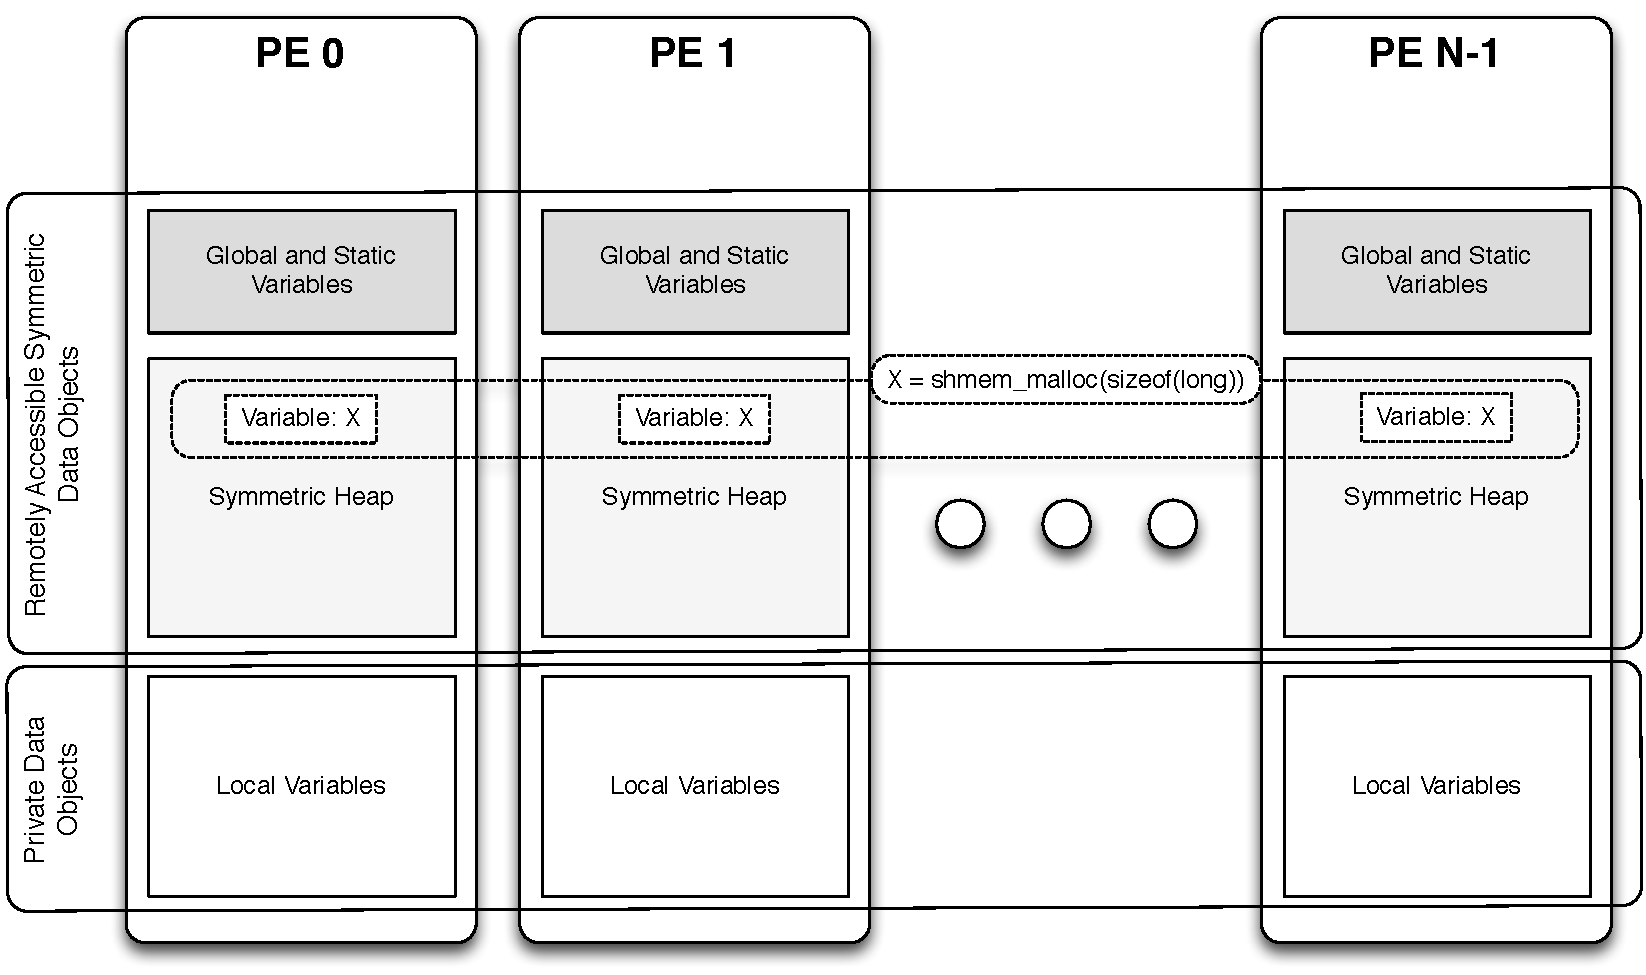
\includegraphics[width=0.95\textwidth]{figures/mem_model}
\caption{\openshmem Memory Model}
\label{fig:mem_model}
\end{figure}
%
An \openshmem program consists of data objects that are private to each \ac{PE}
and data  objects that are remotely accessible by all \acp{PE}. Private data
objects are stored in the local memory of each \ac{PE} and can only be accessed
by the \ac{PE} itself; these data objects cannot be accessed by other \acp{PE}
via \openshmem routines. Private data objects follow the memory model of
\Cstd. Remotely accessible objects, however, can be accessed by
remote \acp{PE} using \openshmem routines.  Remotely accessible data objects are
called \emph{Symmetric Data Objects}.  Each symmetric data object has a
corresponding object with the same name, type, and size on all \acp{PE} where that object is
accessible via the \openshmem \ac{API}\footnote{For efficiency reasons,
the same offset (from an arbitrary memory address) for symmetric data
objects might be used on all \acp{PE}. Further discussion about symmetric heap
layout and implementation efficiency can be found in section
\ref{subsec:shfree}}.  (For the definition of what is accessible, see the
descriptions for \FUNC{shmem\_pe\_accessible} and \FUNC{shmem\_addr\_accessible}
in sections \ref{subsec:shmem_pe_accessible} and
\ref{subsec:shmem_addr_accessible}.) In \openshmem the following kinds of
data objects are symmetric:
%
\begin{itemize}
\item Global and static \Cstd and \Cpp variables. These data objects must
  not be defined in a dynamic shared object (DSO).
\item \Cstd and \Cpp data allocated by \openshmem memory management routines
  (Section~\ref{sec:memory_management})
\end{itemize}

\openshmem dynamic memory allocation routines (e.g.,
\FUNC{shmem\_malloc}) allow collective allocation of \emph{Symmetric Data
Objects} on a special memory region called the \emph{Symmetric Heap}. The
Symmetric Heap is created during the execution of a program at a memory location
determined by the implementation. The Symmetric Heap may reside in different
memory regions on different \acp{PE}.
Figure~\ref{fig:mem_model} shows an example \openshmem
memory layout, illustrating the location of remotely accessible symmetric
objects and private data objects.  As shown, symmetric data objects can be
located either in the symmetric heap or in the global/static memory section of
each \ac{PE}.

\subsection{Pointers to Symmetric Objects}

Symmetric data objects are referenced in \openshmem operations through the
local pointer to the desired remotely accessible object.  The address contained
in this pointer is referred to as a {\em symmetric address}.  Every symmetric
address is also a {\em local address} that is valid for direct memory access;
however, not all local addresses are symmetric.  Manipulation of symmetric
addresses passed to \openshmem routines, including pointer arithmetic;
structure or union member access; and array indexing are permitted as long as
the resulting local pointer remains within the same symmetric allocation or
object.  Symmetric addresses are only valid at the \ac{PE} where they were
generated; using a symmetric address generated by a different \ac{PE} for
direct memory access or as an argument to an \openshmem routine results
in undefined behavior.

Symmetric addresses provided to typed and type-generic \openshmem interfaces
must be naturally aligned based on their type and any requirements of the
underlying architecture.  Symmetric addresses provided to fixed-size (e.g.
\FUNC{shmem\_put32}) \openshmem interfaces must also be aligned to the given
size.  The ``mem'' interfaces, e.g. \FUNC{shmem\_putmem} have no alignment
requirements.  Symmetric objects provided to fixed-size \openshmem interfaces
must have storage size equal to the bit-width of the given
operation\footnote{The bit-width of a byte is implementation-defined in C.  The
\CONST{CHAR\_BIT} constant in \HEADER{limits.h} can be used to portably
calculate the bit-width of a C object.}.  Because \CorCpp{} structures may
contain implementation-defined padding, the fixed-size interfaces should not be
used with \CorCpp{} structures.

The \FUNC{shmem\_ptr} routine allows the programmer to query a {\em local
address} to a remotely accessible data object at a specified \ac{PE}.  The
resulting pointer is valid for direct memory access; however, providing this
address as an argument of an \openshmem routine that requires a symmetric
address results in undefined behavior.

\subsection{Atomicity Guarantees}\label{subsec:amo_guarantees}

\openshmem contains a number of routines that perform atomic operations on
symmetric data objects, which are defined in Section~\ref{sec:amo}.
The atomic routines
guarantee that concurrent accesses by any of these routines to the same
location, using the same datatype (specified in Tables~\ref{stdamotypes} and
\ref{extamotypes}), and using communication contexts (see Section~\ref{sec:ctx})
in the same atomicity domain will be exclusive.
Exclusivity is also guaranteed when the target \ac{PE} performs a wait or test
operation on the same location and with the same datatype as one or more atomic
operations.

An \openshmem \emph{atomicity domain} is a set of communication
contexts whose associated teams (see Section~\ref{subsec:team}) are
all split by (possibly recursive) calls to a
\FUNC{shmem\_team\_split\_*} routine from a common predefined team.
\openshmem defines two such predefined teams, \LibHandleRef{SHMEM\_TEAM\_WORLD}
and \LibHandleRef{SHMEM\_TEAM\_SHARED} (see Section~\ref{subsec:library_handles}).%
\footnote{
  Although all \acp{PE} in \LibHandleRef{SHMEM\_TEAM\_SHARED} are also
  in \LibHandleRef{SHMEM\_TEAM\_WORLD}, and a \ac{PE}'s number can be
  translated from its \LibHandleRef{SHMEM\_TEAM\_SHARED} to
  \LibHandleRef{SHMEM\_TEAM\_WORLD}, the
  \LibHandleRef{SHMEM\_TEAM\_SHARED} team is defined as not having
  been created by a call to a \FUNC{shmem\_team\_split\_*} routine on
  \LibHandleRef{SHMEM\_TEAM\_WORLD}.
  Therefore, the two teams are distinct predefined teams forming
  separate atomicity domains.
}

\openshmem atomic operations do not guarantee exclusivity in the following
scenarios, all of which result in undefined behavior.
\begin{enumerate}
    \item When concurrent accesses to the same location are performed using
        \openshmem atomic operations using communication contexts in
        different atomicity domains.
    \item When concurrent accesses to the same location are performed using
        \openshmem atomic operations using different datatypes.
    \item When atomic and non-atomic \openshmem operations are used to access
        the same location concurrently.
    \item When \openshmem atomic operations and non-\openshmem operations (e.g.
        load and store operations) are used to access the same location
        concurrently.
\end{enumerate}
For example, during the execution of an atomic remote integer increment, i.e. \FUNC{shmem\_atomic\_inc},
operation on a symmetric variable \VAR{X}, no other \openshmem atomic operation
may access \VAR{X}.  After the increment, \VAR{X} will have increased its value
by \CONST{1} on the destination \ac{PE}, at which point other atomic operations
may then modify that \VAR{X}.  However, access to the symmetric object \VAR{X}
with non-atomic operations, such as one-sided \OPR{put} or \OPR{get} operations,
will invalidate the atomicity guarantees.

\cexample
    {
      The following \CorCpp example illustrates scenario 1.
      In this example, different atomicity domains are used to access
      the same location, resulting in undefined behavior.
      The undefined behavior can be resolved by using communication
      contexts in the same atomicity domain in all concurrent operations.
    } {./example_code/amo_scenario_1.c}

\cexample
    {The following \CorCpp example illustrates scenario 2.  In this example,
    different datatypes are used to access the same location concurrently,
    resulting in undefined behavior.  The undefined behavior can be resolved by
    using the same datatype in all concurrent operations.  For example, the
    32-bit value can be left-shifted and a 64-bit atomic OR operation can be
    used.}
    {./example_code/amo_scenario_2.c}

\cexample
    {The following \CorCpp example illustrates scenario 3.  In this example,
    atomic increment operations are concurrent with a non-atomic reduction
    operation, resulting in undefined behavior.  The undefined behavior can be
    resolved by inserting a barrier operation before the reduction.  The
    barrier ensures that all local and remote AMOs have completed before the
    reduction operation accesses $x$.}
    {./example_code/amo_scenario_3.c}

\cexample
    {The following \CorCpp example illustrates scenario 4.  In this example, an
    \openshmem atomic increment operation is concurrent with a local increment
    operation, resulting in undefined behavior.  The undefined behavior can be
    resolved by replacing the local increment operation with an \openshmem
    atomic increment.}
    {./example_code/amo_scenario_4.c}


\section{Execution Model}\label{subsec:execution_model}
An \openshmem program consists of a set of \openshmem processes called \acp{PE}
that execute in a \ac{SPMD}-like model where each \ac{PE} can take a different
execution path. For example, a \ac{PE} can be implemented using an OS
process.  The \acp{PE} progress asynchronously, and can communicate/synchronize
via the \openshmem interfaces.  All \acp{PE} in an \openshmem program should
start by calling the initialization routine  \FUNC{shmem\_init}
\footnote{\textbf{start\_pes} has been deprecated as of Specification 1.2}
before using any of the other \openshmem library routines.  An \openshmem
program finishes execution by returning from the main routine, or when any PE
calls \FUNC{shmem\_global\_exit}. When returning from main, \openshmem must
complete all pending communication and release all the resources associated to
the library using an implicit collective synchronization across PEs. The user
has the option to call \FUNC{shmem\_finalize} (before returning from main) to
complete all pending communication and release all the \openshmem library
resources without terminating the program. Calling any \openshmem routine after
\FUNC{shmem\_finalize} leads to undefined behavior.

The \acp{PE} of the \openshmem program are identified by unique integers.  The
identifiers are integers assigned in a monotonically increasing manner from zero
to the total number of \acp{PE} minus 1. \ac{PE} identifiers are used for
\openshmem calls (e.g. to specify \OPR{put} or \OPR{get} routines on symmetric
data objects, collective synchronization calls) or to dictate a control flow for
\acp{PE} using constructs of \Cstd or \Fortran. The identifiers are fixed for
the life of the \openshmem program.

\subsection{Progress of \openshmem Operations}\label{subsec:progress}

The \openshmem model assumes that computation and communication are naturally
overlapped. \openshmem programs are expected to exhibit progression of
communication both with and without \openshmem calls. Consider a \ac{PE} that is
engaged in a computation with no \openshmem calls. Other \acp{PE} should be able
to communicate (\OPR{put}, \OPR{get}, \OPR{collective}, \OPR{atomic}, etc) and
complete communication operations with that computationally-bound \ac{PE}
without that \ac{PE} issuing any explicit \openshmem calls. \openshmem
communication calls involving that \ac{PE} should progress regardless of when
that \ac{PE} next engages in an \openshmem call.

\textbf{Note to implementors:}
\begin{itemize}
  \item An \openshmem implementation for hardware that does not provide
      asynchronous communication capabilities may require a software progress
      thread in order to process remotely-issued communication requests without
      explicit program calls to the \openshmem library.  
  \item High performance implementations of \openshmem are expected to leverage
      hardware offload capabilities and provide asynchronous one-sided
      communication without software assistance.
  \item Implementations should avoid deferring the execution of one-sided
      operations until a synchronization point where data is known to be
      available. High-quality implementations should attempt asynchronous delivery
      whenever possible, for performance reasons. Additionally, the \openshmem
      community discourages releasing \openshmem implementations that do not
      provide asynchronous one-sided operations, as these have very limited
      performance value for \openshmem programs.
\end{itemize}

\subsection{Atomicity Guarantees}\label{subsec:amo_guarantees}

\openshmem contains a number of routines that operate on symmetric data
atomically (Section \ref{sec:amo}).  These routines guarantee that accesses by
\openshmem's atomic operations with the same datatype will be exclusive, but do not guarantee
exclusivity in combination with other routines, either inside \openshmem or
outside.

For example: during the execution of an atomic remote integer increment
operation on a symmetric variable \VAR{X}, no other \openshmem atomic operation
may access \VAR{X}.  After the increment, \VAR{X} will have increased its value
by \CONST{1} on the destination \ac{PE}, at which point other atomic operations
may then modify that \VAR{X}.  However, access to the symmetric object \VAR{X}
with non-atomic operations, such as one-sided \OPR{put} or \OPR{get} operations,
will \OPR{invalidate} the atomicity guarantees.


\section{Language Bindings and Conformance}\label{subsec:bindings}
\openshmem provides ISO \Cstd language bindings. Any implementation that
provides \Cstd bindings can claim conformance to the specification. The
\openshmem header file \HEADER{shmem.h} for \Cstd must contain only the
interfaces and constant names defined in this specification.

\openshmem \acp{API} can be implemented as functions, inline functions, or
macros. However, implementing the interfaces using inline functions or macros
could limit the use of external profiling tools and high-level compiler
optimizations. An \openshmem program should avoid defining routine names,
variables, or other identifiers with the prefix ``shmem'' using any combination
of uppercase letters, lowercase letters, and underscores.

All extensions to the \openshmem \ac{API} that are not part of this
specification must be defined in the \HEADER{shmemx.h} header file, with the
following exceptions.

\begin{enumerate}
    \item Extensions to the \openshmem interfaces that add support for
        additional datatypes.
    \item Implementation-specific constants, types, and macros that use a
        consistent, implementation-defined prefix.
    \item Extensions to the type-generic interfaces.
\end{enumerate}

The \HEADER{shmemx.h}
header file must exist, even if no extensions are provided. Any extensions
shall use the \FUNC{shmemx\_} prefix for all routine, variable, and constant
names.


\section{Library Constants}\label{subsec:library_constants}
\TableIndex{Library Constants}
\TableIndex{Constants}

The \openshmem library provides a set of compile-time constants that may
be used to specify options to API routines, provide implementation-specific
parameters, or return information about the implementation.
All constants that start with \CONST{\_SHMEM\_*} are deprecated,
but provided for backwards compatibility.

\begin{longtable}{|p{0.45\textwidth}|p{0.5\textwidth}|}
\hline
\textbf{Constant} & \textbf{Description}
\tabularnewline \hline
\endhead
%%
\LibConstDecl{SHMEM\_THREAD\_SINGLE} &
The \openshmem thread support level which specifies that the program
must not be multithreaded.
See Section~\ref{subsec:thread_support} for more detail about its use.
\tabularnewline \hline
%%
\LibConstDecl{SHMEM\_THREAD\_FUNNELED} &
The \openshmem thread support level which specifies that the program
may be multithreaded but must ensure that only the main thread invokes
the \openshmem interfaces.
See Section~\ref{subsec:thread_support} for more detail about its use.
\tabularnewline \hline
%%
\LibConstDecl{SHMEM\_THREAD\_SERIALIZED} &
The \openshmem thread support level which specifies that the program
may be multithreaded but must ensure that the \openshmem interfaces
are not invoked concurrently by multiple threads.
See Section~\ref{subsec:thread_support} for more detail about its use.
\tabularnewline \hline
%%
\LibConstDecl{SHMEM\_THREAD\_MULTIPLE} &
The \openshmem thread support level which specifies that the program
may be multithreaded and any thread may invoke the \openshmem interfaces.
See Section~\ref{subsec:thread_support} for more detail about its use.
\tabularnewline \hline
%%
\color{Green}
\LibConstDecl{SHMEM\_TEAM\_NUM\_CONTEXTS} &
\color{Green}
The bitwise flag which specifies that a team creation routine should use the
\VAR{num\_contexts} member of the provided
\CTYPE{shmem\_team\_config\_t} configuration parameter as a request.
See Sections~\ref{subsec:shmem_team_config_t} and
\ref{subsec:shmem_team_split_strided} for more detail about its use.
\tabularnewline \hline
%%
\color{Green}
\LibConstDecl{SHMEM\_TEAM\_INVALID} &
\color{Green}
A value corresponding to an invalid team.
This value can be used to initialize or update team handles to indicate
that they do not reference a valid team.
When managed in this way, applications can use an equality comparison
to test whether a given team handle references a valid team.
See Section~\ref{subsec:team} for more detail about its use.
\tabularnewline \hline
%%
\LibConstDecl{SHMEM\_CTX\_INVALID} &
A value corresponding to an invalid communication context.
This value can be used to initialize or update context handles to indicate
that they do not reference a valid context.
When managed in this way, applications can use an equality comparison
to test whether a given context handle references a valid context.
See Section~\ref{sec:ctx} for more detail about its use.
\tabularnewline \hline
%%
\LibConstDecl{SHMEM\_CTX\_SERIALIZED} &
The context creation option which specifies that the given context
is shareable but will not be used by multiple threads concurrently.
See Section~\ref{subsec:shmem_ctx_create} for more detail about its use.
\tabularnewline \hline
%%
\LibConstDecl{SHMEM\_CTX\_PRIVATE} &
The context creation option which specifies that the given context
will be used only by the thread that created it.
See Section~\ref{subsec:shmem_ctx_create} for more detail about its use.
\tabularnewline \hline
%%
\LibConstDecl{SHMEM\_CTX\_NOSTORE} &
The context creation option which specifies that quiet and fence operations
performed on the given context are not required to enforce completion and
ordering of memory store operations.
See Section~\ref{subsec:shmem_ctx_create} for more detail about its use.
\tabularnewline \hline
%%
\LibConstDecl{SHMEM\_SYNC\_VALUE}
\begin{DeprecateBlock}
  \LibConstDecl{\_SHMEM\_SYNC\_VALUE}
\end{DeprecateBlock}
&
The value used to initialize the elements of \VAR{pSync} arrays.
The value of this constant is implementation specific.
See Section~\ref{subsec:coll} for more detail about its use.
\tabularnewline \hline
%%
\LibConstDecl{SHMEM\_SYNC\_SIZE}
&
Length of a work array that can be used with any SHMEM collective
communication operation.
Work arrays sized for specific operations may consume less memory.
The value of this constant is implementation specific.
See Section~\ref{subsec:coll} for more detail about its use.
\tabularnewline \hline
%%
\LibConstDecl{SHMEM\_BCAST\_SYNC\_SIZE}
\begin{DeprecateBlock}
  \LibConstDecl{\_SHMEM\_BCAST\_SYNC\_SIZE}
\end{DeprecateBlock}
&
Length of the \VAR{pSync} arrays needed for broadcast routines. The value
of this constant is implementation specific.
See Section~\ref{subsec:shmem_broadcast} for more detail about its use.
\tabularnewline \hline
%%
\LibConstDecl{SHMEM\_REDUCE\_SYNC\_SIZE}
\begin{DeprecateBlock}
  \LibConstDecl{\_SHMEM\_REDUCE\_SYNC\_SIZE}
\end{DeprecateBlock}
&
Length of the work arrays needed for reduction routines.
The value of this constant is implementation specific.
See Section~\ref{subsec:shmem_reductions} for more detail about its use.
\tabularnewline \hline
%%
\LibConstDecl{SHMEM\_BARRIER\_SYNC\_SIZE}
\begin{DeprecateBlock}
  \LibConstDecl{\_SHMEM\_BARRIER\_SYNC\_SIZE}
\end{DeprecateBlock}
&
Length of the work array needed for barrier routines.
The value of this constant is implementation specific.
See Section~\ref{subsec:shmem_barrier} for more detail about its use.

\tabularnewline \hline
%%
\LibConstDecl{SHMEM\_COLLECT\_SYNC\_SIZE}
\begin{DeprecateBlock}
  \LibConstDecl{\_SHMEM\_COLLECT\_SYNC\_SIZE}
\end{DeprecateBlock}
&
Length of the work array needed for collect routines.
The value of this constant is implementation specific.
See Section~\ref{subsec:shmem_collect} for more detail about its use.
\tabularnewline \hline
%%
\LibConstDecl{SHMEM\_ALLTOALL\_SYNC\_SIZE}
\begin{DeprecateBlock}
\end{DeprecateBlock}
&
Length of the work array needed for \FUNC{shmem\_alltoall} routines.
The value of this constant is implementation specific.
See Section~\ref{subsec:shmem_alltoall} for more detail about its use.
\tabularnewline \hline
%%
\LibConstDecl{SHMEM\_ALLTOALLS\_SYNC\_SIZE}
\begin{DeprecateBlock}
\end{DeprecateBlock}
&
Length of the work array needed for \FUNC{shmem\_alltoalls} routines.
The value of this constant is implementation specific.
See Section~\ref{subsec:shmem_alltoalls} for more detail about its use.
\tabularnewline \hline
%%
\LibConstDecl{SHMEM\_REDUCE\_MIN\_WRKDATA\_SIZE}
\begin{DeprecateBlock}
  \LibConstDecl{\_SHMEM\_REDUCE\_MIN\_WRKDATA\_SIZE}
\end{DeprecateBlock}
&
Minimum length of work arrays used in various collective routines.
\tabularnewline \hline
%%
\LibConstDecl{SHMEM\_MAJOR\_VERSION}
\begin{DeprecateBlock}
  \LibConstDecl{\_SHMEM\_MAJOR\_VERSION}
\end{DeprecateBlock}
&
Integer representing the major version of \openshmem Specification in use.
\tabularnewline \hline
%%
\LibConstDecl{SHMEM\_MINOR\_VERSION}
\begin{DeprecateBlock}
  \LibConstDecl{\_SHMEM\_MINOR\_VERSION}
\end{DeprecateBlock}
&
Integer representing the minor version of \openshmem Specification in use.
\tabularnewline \hline
%%
\LibConstDecl{SHMEM\_MAX\_NAME\_LEN}
\begin{DeprecateBlock}
  \LibConstDecl{\_SHMEM\_MAX\_NAME\_LEN}
\end{DeprecateBlock}
&
Integer representing the maximum length of \CONST{SHMEM\_VENDOR\_STRING}.
\tabularnewline \hline
%%
\LibConstDecl{SHMEM\_VENDOR\_STRING}
\begin{DeprecateBlock}
  \LibConstDecl{\_SHMEM\_VENDOR\_STRING}
\end{DeprecateBlock}
&
String representing vendor defined information of size at most
\CONST{SHMEM\_MAX\_NAME\_LEN}.
In \CorCpp{}, the string is terminated by a null character.
\tabularnewline \hline
%%
\LibConstDecl{SHMEM\_CMP\_EQ}
\begin{DeprecateBlock}
  \LibConstDecl{\_SHMEM\_CMP\_EQ}
\end{DeprecateBlock}
&
An integer constant expression corresponding to the
``equal to'' comparison operation.
See Section~\ref{subsec:p2p_intro} for more detail about its use.
\tabularnewline \hline
%%
\LibConstDecl{SHMEM\_CMP\_NE}
\begin{DeprecateBlock}
  \LibConstDecl{\_SHMEM\_CMP\_NE}
\end{DeprecateBlock}
&
An integer constant expression corresponding to the
``not equal to'' comparison operation.
See Section~\ref{subsec:p2p_intro} for more detail about its use.
\tabularnewline \hline
%%
\LibConstDecl{SHMEM\_CMP\_LT}
\begin{DeprecateBlock}
  \LibConstDecl{\_SHMEM\_CMP\_LT}
\end{DeprecateBlock}
&
An integer constant expression corresponding to the
``less than'' comparison operation.
See Section~\ref{subsec:p2p_intro} for more detail about its use.
\tabularnewline \hline
%%
\LibConstDecl{SHMEM\_CMP\_LE}
\begin{DeprecateBlock}
  \LibConstDecl{\_SHMEM\_CMP\_LE}
\end{DeprecateBlock}
&
An integer constant expression corresponding to the
``less than or equal to'' comparison operation.
See Section~\ref{subsec:p2p_intro} for more detail about its use.
\tabularnewline \hline
%%
\LibConstDecl{SHMEM\_CMP\_GT}
\begin{DeprecateBlock}
  \LibConstDecl{\_SHMEM\_CMP\_GT}
\end{DeprecateBlock}
&
An integer constant expression corresponding to the
``greater than'' comparison operation.
See Section~\ref{subsec:p2p_intro} for more detail about its use.
\tabularnewline \hline
%%
\LibConstDecl{SHMEM\_CMP\_GE}
\begin{DeprecateBlock}
  \LibConstDecl{\_SHMEM\_CMP\_GE}
\end{DeprecateBlock}
&
An integer constant expression corresponding to the
``greater than or equal to'' comparison operation.
See Section~\ref{subsec:p2p_intro} for more detail about its use.
\tabularnewline \hline
%%
\end{longtable}


\section{Environment Variables }\label{subsec:environment_variables}
\TableIndex{Environment Variables}

The \openshmem specification provides a set of environment variables that allows
users to configure the \openshmem implementation, and receive information about
the implementation. The implementations of the specification are free to define
additional variables. Currently, the specification defines four environment
variables. All environment variables that start with \VAR{SMA\_*} are
deprecated, but currently supported for backwards compatibility.
If both \VAR{SHMEM\_}- and \VAR{SMA\_}-prefixed environment variables
are set, then the value in the \VAR{SHMEM\_}-prefixed environment variable
establishes the controlling value. Refer to the
\hyperref[subsec:deprecate-sma-env]{\VAR{SMA\_*} Environment Variables}
deprecation rationale for more details.

\medskip{}

\begin{longtable}{|p{0.260\textwidth}|p{0.145\textwidth}|p{0.50\textwidth}|}
\hline
\textbf{Variable} & \textbf{Value} & \textbf{Description}
\tabularnewline\hline
%%
\EnvVarDecl{SHMEM\_VERSION}
    & Any
    & Print the library version at start-up
    \tabularnewline\hline
%%
\EnvVarDecl{SHMEM\_INFO}
    & Any
    & Print helpful text about all these environment variables
    \tabularnewline\hline
%%
\EnvVarDecl{SHMEM\_SYMMETRIC\_SIZE}
    & Positive decimal value (integer or floating point) with an optional
    character suffix %that specifies a scaling factor
    & The value set in this environment variable is interpreted as an
    implementation-defined size (in bytes) at least as large as the integer
    ceiling of the product of the numeric prefix and the scaling factor. The
    allowed character suffix for the scaling factor are as follows:
      \begin{itemize}
        \item k or K multiplies by \(2^{10}\)  (kibibytes)
        \item m or M multiplies by \(2^{20}\)  (mebibytes)
        \item g or G multiplies by \(2^{30}\)  (gibibytes)
        \item t or T multiplies by \(2^{40}\)  (tebibytes)
      \end{itemize}
      For example, string \enquote{20m} is equivalent to the integer value
      20971520, or 20 megabytes. Similarly the string \enquote{3.1m} is
      equivalent to the integer value 3250586. Only one multiplier is
      recognized, so \enquote{20kk} will not produce the same desired result as
      \enquote{20m}. Usage of string \enquote{.5m} will yield the same result as
      the string \enquote{0.5m}. Any unrecognized suffix is an error, generates
      an error report, and either returns from shmem_init_thread or otherwise
      causes program termination.
    \tabularnewline\hline
%%
\EnvVarDecl{SHMEM\_DEBUG}
    & Any
    & Enable debugging messages
    \tabularnewline\hline
\end{longtable}

\medskip{}





\clearpage



\section{OpenSHMEM Library API}\label{sec:openshmem_library_api}

\subsection{Library Setup, Exit, and Query Routines}
The library setup and query interfaces that initialize and monitor the parallel
environment of the \ac{PE}s.

\subsubsection{\textbf{SHMEM\_INIT}}\label{subsec:shmem_init}
\apisummary{
    A collective operation that allocates and initializes the resources used by
    the \openshmem library.
}

\begin{apidefinition}

\begin{Csynopsis}
void shmem_init(void);
\end{Csynopsis}

\begin{Fsynopsis}
CALL SHMEM_INIT()
\end{Fsynopsis}


\begin{apiarguments}
    \apiargument{None.}{}{}
\end{apiarguments}

\apidescription{
    \FUNC{shmem\_init} allocates and initializes resources used by the \openshmem
    library. It is a collective operation that all \acp{PE} must call before any
    other \openshmem routine may be called. At the end of the \openshmem program
    which it initialized, the call to \FUNC{shmem\_init} must be matched with a
    call to \FUNC{shmem\_finalize}. After the first call to \FUNC{shmem\_init}, a
    subsequent call to \FUNC{shmem\_init} or \FUNC{shmem\_init\_thread} in the
    same program results in undefined behavior.
}

\apireturnvalues{
    None.
}      

\apinotes{
    As of \openshmem[1.2], the use of \FUNC{start\_pes} has been
    deprecated and is replaced with \FUNC{shmem\_init}. While support for
    \FUNC{start\_pes} is still required in \openshmem libraries, users are
    encouraged to use \FUNC{shmem\_init}. An important difference between
    \FUNC{shmem\_init} and \FUNC{start\_pes} is that multiple calls to
    \FUNC{shmem\_init} within a program results in undefined behavior, while in the
    case of \FUNC{start\_pes}, any subsequent calls to \FUNC{start\_pes} after the
    first one results in a no-op.
}

\begin{apiexamples}

\apifexample
{ The following \FUNC{shmem\_init} example is for \Cstd[11] programs: }
    { example_code/shmem_init_example.c }
    {}

\end{apiexamples}

\end{apidefinition}


\subsubsection{\textbf{SHMEM\_MY\_PE}}\label{subsec:shmem_my_pe}
\apisummary{
    Returns the number of the calling \ac{PE}.
}

\begin{apidefinition}

\begin{Csynopsis}
int shmem_my_pe(void);
\end{Csynopsis}

\begin{Fsynopsis}
INTEGER SHMEM_MY_PE, ME
ME = SHMEM_MY_PE()
\end{Fsynopsis}

\begin{apiarguments}
    \apiargument{None.}{}{}
\end{apiarguments}

\apidescription{
    This routine returns the \ac{PE} number of the calling \ac{PE}.  It accepts no
    arguments.  The result is an integer between \CONST{0} and \VAR{npes} -
    \CONST{1}, where \VAR{npes} is the total number of \ac{PE}s executing the
    current program.
}

\apireturnvalues{
    Integer - Between \CONST{0} and \VAR{npes} - \CONST{1}
}

\apinotes{
    Each \ac{PE} has a unique number or identifier. As of \openshmem Specification
    1.2 the use of \FUNC{\_my\_pe} has been deprecated. Although \openshmem
    libraries are required to support the call, users are encouraged to use
    \FUNC{shmem\_my\_pe} instead.  The behavior and signature  of the routine
    \FUNC{shmem\_my\_pe} remains unchanged from the deprecated \FUNC{\_my\_pe}
    version.
}

\begin{apiexamples}

\apicexample
    {The following \FUNC{shmem\_my\_pe} example is for \CorCpp{} programs:}
    {./example_code/shmem_mype_example.c}
    {}

\end{apiexamples}

\end{apidefinition}


\subsubsection{\textbf{SHMEM\_N\_PES}}\label{subsec:shmem_n_pes}
\apisummary{
    Returns the number of \ac{PE}s running in a program.
}

\begin{apidefinition}

\begin{Csynopsis}
int shmem_n_pes(void);
\end{Csynopsis}

\begin{Fsynopsis}
INTEGER SHMEM_N_PES, N_PES
N_PES = SHMEM_N_PES()
\end{Fsynopsis}

\begin{apiarguments}
    \apiargument{None.}{}{}
\end{apiarguments}

\apidescription{
    The routine returns the number of \ac{PE}s running in the program.
}

\apireturnvalues{
    Integer -  Number of \ac{PE}s running in the \openshmem program.
}

\apinotes{
    As of \openshmem Specification 1.2 the use of \FUNC{\_num\_pes} has been
    deprecated. Although \openshmem libraries are required to support the call,
    users are encouraged to use \FUNC{shmem\_n\_pes} instead.  The behavior and
    signature  of the routine \FUNC{shmem\_n\_pes} remains unchanged from the
    deprecated \FUNC{\_num\_pes} version.
}

\begin{apiexamples}

\apicexample
    {The following \FUNC{shmem\_n\_pes} example is for \CorCpp{} programs:}
    {./example_code/shmem_npes_example.c}
    {}

\end{apiexamples}

\end{apidefinition}


\subsubsection{\textbf{SHMEM\_FINALIZE}}\label{subsec:shmem_finalize}
\apisummary{
    A collective operation that releases resources used by the \openshmem
    library.  This only terminates the \openshmem portion of a program, not the
    entire program.
}

\begin{apidefinition}

\begin{Csynopsis}
void shmem_finalize(void);
\end{Csynopsis}

\begin{Fsynopsis}
CALL SHMEM_FINALIZE()
\end{Fsynopsis}

\begin{apiarguments}
    \apiargument{None.}{}{}
\end{apiarguments}

\apidescription{
    \FUNC{shmem\_finalize} is a collective operation that ends the \openshmem
    portion of a program previously initialized by \FUNC{shmem\_init} and
    releases resources used by the \openshmem library. This collective
    operation requires all \acp{PE} to participate in the call. There is an
    implicit global barrier in \FUNC{shmem\_finalize} so that pending
    communications \newtext{by all threads of the \ac{PE}} are completed, and no resources can be released until all
    \acp{PE} have entered \FUNC{shmem\_finalize}. \FUNC{shmem\_finalize} must be
    the last \openshmem library call encountered in the \openshmem portion of a
    program. A call to \FUNC{shmem\_finalize} will release any resources
    initialized by a corresponding call to \FUNC{shmem\_init}. All processes
    that represent the \acp{PE} will still exist after the
    call to \FUNC{shmem\_finalize} returns, but they will no longer have access
    to any resources that have been released.
}

\apireturnvalues{
    None.
}

\apinotes{
    \FUNC{shmem\_finalize} releases all resources used by the \openshmem library
    including the symmetric memory heap and pointers initiated by
    \FUNC{shmem\_ptr}. This collective operation requires all \acp{PE} to
    participate in the call, not just a subset of the \acp{PE}. The
    non-\openshmem portion of a program may continue after a call to
    \FUNC{shmem\_finalize} by all \acp{PE}. There is an implicit
    \FUNC{shmem\_finalize} at the end of main, so that having an explicit call
    to \FUNC{shmem\_finalize} is optional. However, an explicit
    \FUNC{shmem\_finalize} may be required as an entry point for wrappers used
    by profiling or other tools that need to perform their own finalization.
}

\begin{apiexamples}

\apicexample
    {The following finalize example is for C11 programs:}
    {./example_code/shmem_finalize_example.c}
    {}

\end{apiexamples}

\end{apidefinition}


\subsubsection{\textbf{SHMEM\_GLOBAL\_EXIT}}\label{subsec:shmem_global_exit}
\apisummary{
    A routine that allows any \ac{PE} to force termination of an entire program.
}

\begin{apidefinition}

\begin{C11synopsis}
_Noreturn void shmem_global_exit(int status);
\end{C11synopsis}

\begin{Csynopsis}
void shmem_global_exit(int status);
\end{Csynopsis}

\begin{DeprecateBlock}
\begin{Fsynopsis}
INTEGER STATUS
CALL SHMEM_GLOBAL_EXIT(status)
\end{Fsynopsis}
\end{DeprecateBlock}

\begin{apiarguments}
    \apiargument{IN}{status}{The exit status from the main program.}
\end{apiarguments}

\apidescription{
    \FUNC{shmem\_global\_exit} is a non-collective routine that allows any one
    \ac{PE} to force termination of an \openshmem program for all \acp{PE},
    passing an exit status to the execution environment. This routine terminates
    the entire program, not just the \openshmem portion.  When any \ac{PE} calls
    \FUNC{shmem\_global\_exit}, it results in the immediate notification to all
    \acp{PE} to terminate.  \FUNC{shmem\_global\_exit} flushes I/O and releases
    resources in accordance with C/C++/Fortran language requirements for normal
    program termination. If more than one \ac{PE} calls
    \FUNC{shmem\_global\_exit}, then the exit status returned to the environment
    shall be one of the values passed to \FUNC{shmem\_global\_exit} as the
    status argument.  There is no return to the caller of
    \FUNC{shmem\_global\_exit}; control is returned from the \openshmem program
    to the execution environment for all \acp{PE}.
}

\apireturnvalues{
    None.
}


\apinotes{ 
    \FUNC{shmem\_global\_exit} may be used in situations where one or more
    \acp{PE} have determined that the program has completed and/or should
    terminate early.  Accordingly, the integer status argument can be used to
    pass any information about the nature of the exit, e.g an encountered error
    or a found solution.  Since \FUNC{shmem\_global\_exit} is a non-collective
    routine, there is no implied synchronization, and all \acp{PE} must
    terminate regardless of their current execution state. While I/O must be
    flushed for standard language I/O calls from C/C++/Fortran, it is
    implementation dependent as to how I/O done by other means (e.g. third
    party I/O libraries) is handled. Similarly, resources are released
    according to C/C++/Fortran standard language requirements, but this may not
    include all resources allocated for the \openshmem program. However, a
    quality implementation will make a best effort to flush all I/O and clean
    up all resources.
}

\begin{apiexamples}

\apicexample
    {}
    {./example_code/shmem_global_exit_example.c}
    {}

\end{apiexamples}

\end{apidefinition}


\subsubsection{\textbf{SHMEM\_PE\_ACCESSIBLE}}\label{subsec:shmem_pe_accessible}
\apisummary{
    Determines whether a \ac{PE} is accessible via \openshmem's data transfer
    routines.
}

\begin{apidefinition}

\begin{Csynopsis}
int shmem_pe_accessible(int pe);
\end{Csynopsis}

\begin{Fsynopsis}
LOGICAL LOG, SHMEM_PE_ACCESSIBLE
INTEGER pe
LOG = SHMEM_PE_ACCESSIBLE(pe)
\end{Fsynopsis}

\begin{apiarguments}
    \apiargument{IN}{pe}{Specific \ac{PE} to be checked for accessibility from
    the local \ac{PE}.}
\end{apiarguments}

\apidescription{
    \FUNC{shmem\_pe\_accessible} is  a  query routine  that indicates  whether  a
    specified \ac{PE} is accessible via \openshmem from the local \ac{PE}. The
    \FUNC{shmem\_pe\_accessible} routine returns \CONST{TRUE} only if  the  remote
    \ac{PE} is a process  running from the same executable  file as the local
    \ac{PE}, indicating that full \openshmem support for symmetric data objects
    (that reside in the static memory and symmetric heap) is available, otherwise it
    returns \CONST{FALSE}.  This routine may be particularly useful for hybrid
    programming with other communication libraries (such as a \ac{MPI}) or parallel
    languages.  For example, on  SGI Altix  series  systems, \openshmem is
    supported  across multiple partitioned hosts and InfiniBand connected hosts.
    When running multiple executable MPI programs using \openshmem on an Altix, full
    \openshmem support is available between processes running from the same
    executable file. However, \openshmem support between processes of different
    executable  files  is  supported only for data objects on the symmetric heap,
    since static data objects are  not symmetric  between  different executable
    files.        
}

\apireturnvalues{
    \Clang: The return value is 1 if the specified \ac{PE} is a valid remote \ac{PE}
    for \openshmem routines; otherwise, it is 0. \\ \\

    \Fortran: The return value is \CONST{.TRUE.} if the specified \ac{PE} is a valid
    remote \ac{PE} for \openshmem routines; otherwise, it is \CONST{.FALSE.}.	 
}

\apinotes{ None. }

\end{apidefinition}


\subsubsection{\textbf{SHMEM\_ADDR\_ACCESSIBLE}}\label{subsec:shmem_addr_accessible}
\apisummary{
    Determines whether an address is accessible via OpenSHMEM data transfer
    routines from the specified  remote \ac{PE}.
}

\begin{apidefinition}

\begin{Csynopsis}
int shmem_addr_accessible(const void *addr, int pe);
\end{Csynopsis}

\begin{Fsynopsis}
LOGICAL LOG, SHMEM_ADDR_ACCESSIBLE
INTEGER pe
LOG = SHMEM_ADDR_ACCESSIBLE(addr, pe)
\end{Fsynopsis}

\begin{apiarguments}
    \apiargument{IN}{addr}{Data object on the local \ac{PE}.}
    \apiargument{IN}{pe}{Integer id of a remote \ac{PE}.}
\end{apiarguments}

\apidescription{
    \FUNC{shmem\_addr\_accessible} is a query routine that indicates whether a local
    address is accessible via \openshmem routines from the specified remote \ac{PE}. 
    
    This routine verifies that the data object is symmetric and accessible with
    respect to a remote \ac{PE} via \openshmem  data  transfer routines.  The
    specified address \VAR{addr} is a data object on the local \ac{PE}. 
    
    This routine may be particularly useful for hybrid programming with other
    communication libraries (such as \ac{MPI}) or parallel languages.  For
    example, in SGI Altix series systems, for multiple executable MPI programs that
    use \openshmem routines, it is important to note that static memory, such as a
    \Fortran{} common block or \Cstd global variable, is symmetric between
    processes running from the same executable file, but is not symmetric between
    processes running from different executable files.  Data allocated from the
    symmetric heap (\FUNC{shmem\_malloc} or \FUNC{shpalloc}) is symmetric across the
    same or different executable files.
}

\apireturnvalues{		
    \CorCpp: The  return value is \CONST{1} if \VAR{addr} is a symmetric data object
    and accessible via \openshmem routines from the specified remote \ac{PE};
    otherwise, it is \CONST{0}.
    
    \Fortran: The return value is \CONST{.TRUE.} if \VAR{addr} is a symmetric data
    object and accessible via \openshmem routines from the specified remote \ac{PE};
    otherwise, it is \CONST{.FALSE.}.
}
		
\apinotes{
    None.
}

\end{apidefinition}


\subsubsection{\textbf{SHMEM\_PTR}}\label{subsec:shmem_ptr}
\apisummary{
    Returns a local pointer to a symmetric data object on the specified \ac{PE}.
}

\begin{apidefinition}

\begin{Csynopsis}
void *@\FuncDecl{shmem\_ptr}@(const void *dest, int pe);
\end{Csynopsis}

\begin{apiarguments}
\apiargument{IN}{dest}{The symmetric address of the remotely accessible data
    object to be referenced.}
\apiargument{IN}{pe}{An integer that indicates the \ac{PE} number on which \dest{} is to
    be accessed.}
\end{apiarguments}

\apidescription{
    \FUNC{shmem\_ptr} returns an address that may be used to directly reference
    \dest{} on the specified \ac{PE}.  This address can be assigned to a
    pointer.  After that, ordinary loads and stores to \dest{} may be
    performed.  The address returned by \FUNC{shmem\_ptr} is a local address to
    a remotely accessible data object.  Providing this address to an argument of
    an \openshmem routine that requires a symmetric address results in
    undefined behavior.
    
    The \FUNC{shmem\_ptr} routine can provide an efficient means to accomplish
    communication, for example when a sequence of reads and writes to a data
    object on a remote \ac{PE} does not match the access pattern provided in an
    \openshmem data transfer routine like \FUNC{shmem\_put} or
    \FUNC{shmem\_iget}.
}

\apireturnvalues{
    A local pointer to the remotely accessible \dest{} data object is returned
    when it can be accessed using memory loads and stores.  Otherwise, a null
    pointer is returned.
}

\apinotes{
    When calling \FUNC{shmem\_ptr}, \dest{} is the address of the referenced
    symmetric data object on the calling \ac{PE}.
}

\begin{apiexamples}

\apicexample
    {In the following \Cstd[11] example, \ac{PE} 0 uses the \FUNC{shmem\_ptr}
    routine to query a pointer and directly access the \VAR{dest} array on
    \ac{PE} 1:}
    {./example_code/shmem_ptr_example.c}
    {}

\end{apiexamples}

\end{apidefinition}


\subsubsection{\textbf{SHMEM\_INFO\_GET\_VERSION}}\label{subsec:shmem_info_get_version}
\apisummary{
    Returns the major and minor version of the library implementation.
}

\begin{apidefinition}

\begin{Csynopsis}
void shmem_info_get_version(int *major, int *minor);
\end{Csynopsis}

\begin{Fsynopsis}
INTEGER MAJOR, MINOR
SHMEM_INFO_GET_VERSION(MAJOR, MINOR)   
\end{Fsynopsis}

\begin{apiarguments}
    \apiargument{OUT}{major}{The major version of the \openshmem{} standard in use.}
    \apiargument{OUT}{minor}{The minor version of the \openshmem{} standard in use.}
\end{apiarguments}

\apidescription{
    This routine returns the major and minor version of the \openshmem{} standard
    in use.  For a given library implementation, the major and minor version
    returned by these calls is consistent with the compile-time constants,
    SHMEM\_MAJOR\_VERSION and SHMEM\_MINOR\_VERSION, defined in its shmem.h.  The
    valid major version value is  $1$, and the valid minor version value is $2$. 
}

\apireturnvalues{
    None.
}

\apinotes{
    None. 
}

\end{apidefinition}


\subsubsection{\textbf{SHMEM\_INFO\_GET\_NAME}}\label{subsec:shmem_info_get_name}
\apisummary{
    This routine returns the vendor defined character string.
}

\begin{apidefinition}

\begin{Csynopsis}
void shmem_info_get_name(char *name);
\end{Csynopsis}

\begin{Fsynopsis}
CHARACTER *(*)NAME
SHMEM_INFO_GET_NAME(NAME)   
\end{Fsynopsis}

\begin{apiarguments}
    \apiargument{OUT}{name}{The vendor defined string.}
\end{apiarguments}

\apidescription{
    This routine returns the vendor defined character string of size defined by
    the library constant \CONST{SHMEM\_MAX\_NAME\_LEN}. The program calling
    this function prepares the \VAR{name} memory buffer of at least size
    \CONST{SHMEM\_MAX\_NAME\_LEN}. The implementation copies the vendor defined
    string of size at most \CONST{SHMEM\_MAX\_NAME\_LEN} to \VAR{name}. In
    \CorCpp{}, the string is terminated by a null character.  In \Fortran,
    the string of size less than \CONST{SHMEM\_MAX\_NAME\_LEN} is padded with
    blank characters up to size \CONST{SHMEM\_MAX\_NAME\_LEN}. If the
    \VAR{name} memory buffer is provided with size less than
    \CONST{SHMEM\_MAX\_NAME\_LEN}, behavior is undefined. For a given library
    implementation, the vendor string returned is consistent with the library
    constant \CONST{SHMEM\_VENDOR\_STRING}.
}

\apireturnvalues{ 
    None. 
}

\apinotes{ 
    None. 
}

\end{apidefinition}


\subsubsection{\textbf{START\_PES}}\label{subsec:start_pes}
\apisummary{ 
    Called at the beginning of an \openshmem program to initialize the execution
    environment. This routine is deprecated and is provided for backwards
    compatibility. Implementations must include it, and the routine should
    function properly and may notify the user about deprecation of its use.
}

\begin{apidefinition}

\begin{DeprecateBlock}
\begin{Csynopsis}
void start_pes(int npes);
\end{Csynopsis}
\end{DeprecateBlock}

\begin{Fsynopsis}
CALL START_PES(npes)
\end{Fsynopsis}

\begin{apiarguments}
       \apiargument{npes}{Unused}{ Should be set to \CONST{0}.}
\end{apiarguments}

\apidescription{   
     The \FUNC{start\_pes} routine initializes the \openshmem execution
     environment.  An \openshmem program must call \FUNC{start\_pes},
     \FUNC{shmem\_init}, or \FUNC{shmem\_init\_thread} before calling any other \openshmem routine.  Unlike
     \FUNC{shmem\_init} and \FUNC{shmem\_init\_thread}, \FUNC{start\_pes} does not require a call to
     \FUNC{shmem\_finalize}.  Instead, the \openshmem library is implicitly
     finalized when the program exits.  Implicit finalization is collective and
     includes a global synchronization to ensure that all pending communication
     is completed before resources are released.
}

\apireturnvalues{
    None.
}

\apinotes{
    If any other \openshmem call occurs before \FUNC{start\_pes}, the
    behavior is undefined.  Although it is recommended to set \VAR{npes} to
    \CONST{0} for \FUNC{start\_pes}, this is not mandated.  The value is ignored.
    Calling \FUNC{start\_pes} more than once has no subsequent
    effect.

    As of \openshmem[1.2] the use of \FUNC{start\_pes} has
    been deprecated. Although \openshmem libraries are required to support the
    call, users are encouraged to use \FUNC{shmem\_init} or
    \FUNC{shmem\_init\_thread} instead.
}


\begin{apiexamples}

\apicexample
    { This is a simple program that calls \FUNC{start\_pes}:}
    {./example_code/shmem_startpes_example.f90}
    {} 

\end{apiexamples}

\end{apidefinition}






\subsection{Memory Management Routines}
\openshmem provides a set of \ac{API}s for managing the symmetric heap. The
\ac{API}s allow one to dynamically allocate, deallocate, reallocate and align
symmetric data objects in the symmetric heap, in \Clang{} and \Fortran.

\subsubsection{\textbf{SHMEM\_MALLOC, SHMEM\_FREE, SHMEM\_REALLOC, SHMEM\_ALIGN}}\label{subsec:shfree}
\apisummary{
    Symmetric heap memory management routines.
}

\begin{apidefinition}

\begin{Csynopsis}
void *shmem_malloc(size_t size);
void shmem_free(void *ptr);
void *shmem_realloc(void *ptr, size_t size);
void *shmem_align(size_t alignment, size_t size);
\end{Csynopsis}

\begin{apiarguments}
    \apiargument{IN}{size}{The size, in bytes, of a block to be
        allocated from the symmetric heap. This argument is of type \VAR{size\_t}}
    \apiargument{IN}{ptr}{Points to a block within the symmetric heap.}
    \apiargument{IN}{alignment}{Byte alignment of the block allocated from the
        symmetric heap.}
\end{apiarguments}


\apidescription{
    The \FUNC{shmem\_malloc} routine returns a pointer to a block of at least
    \VAR{size} bytes suitably aligned for any use.  This space is allocated from the
    symmetric heap (in contrast to \FUNC{malloc}, which allocates from the private
    heap).
    
    The \FUNC{shmem\_align} routine allocates a block in the symmetric heap that has
    a byte alignment specified by the alignment argument.
    
    The \FUNC{shmem\_free} routine causes the block to which \VAR{ptr} points to be
    deallocated, that is, made available for further allocation.  If \VAR{ptr} is a
    null pointer, no action occurs. 
           
    The \FUNC{shmem\_realloc} routine changes the size of the block to which
    \VAR{ptr} points to the size (in bytes) specified by \VAR{size}.  The contents
    of the block are unchanged up to the lesser of the new and old sizes. If the new
    size is larger, the newly allocated portion of the block is
    uninitialized.  If \VAR{ptr} is a \CONST{NULL} pointer, the
    \FUNC{shmem\_realloc} routine behaves like the \FUNC{shmem\_malloc} routine for
    the specified size.  If \VAR{size} is \CONST{0} and \VAR{ptr} is not a
    \CONST{NULL} pointer, the block to which it points is freed. If the space cannot
    be allocated, the block to which \VAR{ptr} points is unchanged.
    
    The \FUNC{shmem\_malloc}, \FUNC{shmem\_align}, \FUNC{shmem\_free}, and \FUNC{shmem\_realloc} routines
    are provided  so that multiple \ac{PE}s in a program can allocate symmetric,
    remotely accessible memory blocks.  These memory blocks can then be used with
    \openshmem communication routines.  Each of these routines include at least one
    call to a procedure that is semantically equivalent to \FUNC{shmem\_barrier\_all}:
    \FUNC{shmem\_malloc} and \FUNC{shmem\_align} call a
    barrier on exit; \FUNC{shmem\_free} calls a barrier on entry; and
    \FUNC{shmem\_realloc} may call barriers on both entry and exit, depending on
    whether an existing allocation is modified and whether new memory is allocated.
    This ensures that all
    \ac{PE}s participate in the memory allocation, and that the memory on other
    \ac{PE}s can be used as  soon as the local \ac{PE} returns.
    \newtext{The implicit barriers performed by these routines quiet the
    default context.  It is the user's responsibility to ensure that no
    communication operations involving the given memory block are pending on
    other contexts prior to calling
    the \FUNC{shmem\_free} and \FUNC{shmem\_realloc} routines.}
    The user is \newtext{also}
    responsible for calling these routines with identical argument(s) on all
    \acp{PE}; if differing \VAR{size} arguments are used, the behavior of the call
    and any subsequent \openshmem calls becomes undefined.
}

\apireturnvalues{
    The \FUNC{shmem\_malloc} routine returns a pointer to the allocated space;
    otherwise, it returns a \CONST{NULL} pointer.
    
    The \FUNC{shmem\_free} routine returns no value.
    
    The \FUNC{shmem\_realloc} routine returns a pointer to the allocated space
    (which may have moved); otherwise, it returns a null pointer.
    
    The \FUNC{shmem\_align} routine returns an aligned pointer to the allocated
    space; otherwise, it returns a \CONST{NULL} pointer.
}

\apinotes{ 
    As of Specification 1.2 the use of \FUNC{shmalloc}, \FUNC{shmemalign},
    \FUNC{shfree},  and \FUNC{shrealloc} has been deprecated. Although OpenSHMEM
    libraries are required to support the calls, program users are encouraged to use
    \FUNC{shmem\_malloc}, \FUNC{shmem\_align}, \FUNC{shmem\_free}, and
    \FUNC{shmem\_realloc} instead.  The behavior and signature  of the routines
    remains unchanged from the deprecated versions.
    					 
    The total size of the symmetric heap is determined at job startup.  One can
    adjust the size of the heap using the \CONST{SHMEM\_SYMMETRIC\_SIZE} environment
    variable (where available).	
    
    The \FUNC{shmem\_malloc}, \FUNC{shmem\_free}, and \FUNC{shmem\_realloc} routines
    differ from the private heap allocation routines in that all \acp{PE} in a
    program must call them (a barrier is used to ensure this).
}		

\apiimpnotes{
    The symmetric heap allocation routines always return a pointer to corresponding
    symmetric objects across all PEs. The \openshmem{} specification does not
    require that the virtual addresses are equal across all \acp{PE}. Nevertheless,
    the implementation must avoid costly address translation operations in the
    communication path, including order $N$ (where $N$ is the number of \acp{PE})
    memory translation tables.  In order to avoid address translations, the
    implementation may re-map the allocated block of memory based on agreed virtual
    address.  Additionally, some operating systems provide an option to disable
    virtual address randomization, which enables predictable allocation of virtual
    memory addresses.
}

\end{apidefinition}


\subsubsection{\textbf{SHPALLOC}}\label{subsec:shpalloc}
\apisummary{
    Allocates a block of memory from the symmetric heap.
}

\begin{apidefinition}

\begin{Fsynopsis}
POINTER (addr, A(1))
INTEGER length, errcode, abort
CALL SHPALLOC(addr, length, errcode, abort)
\end{Fsynopsis}

\begin{apiarguments}
    \apiargument{OUT}{addr}{First word address of the allocated block.}
    \apiargument{IN}{length}{Number of words of memory requested. One word is 32 bits.}
    \apiargument{OUT}{errcode}{Error code is \CONST{0} if no error was detected;
    otherwise, it is a negative integer code for the type of error.}
    \apiargument{IN}{abort}{Abort code; nonzero requests abort on error;
    \CONST{0}  requests an error code.}
\end{apiarguments}

\apidescription{   
    \FUNC{SHPALLOC} allocates a block of memory from the program's symmetric heap
    that is greater than or equal to the size requested. To maintain symmetric heap
    consistency, all \ac{PE}s in an program must call \FUNC{SHPALLOC} with the same
    value of length; if any  \ac{PE}s are missing, the program will hang.
    
    By using the \Fortran{} \CONST{POINTER} mechanism in the following manner, you
    can use array \VAR{A} to refer to the block allocated by \FUNC{SHPALLOC}:
    \CONST{POINTER} (\VAR{addr}, \VAR{A}())
}

\apireturnvalues{}
    \apitablerow{Error Code}{Condition}
    \apitablerow{ \CONST{-1} }{Length is not an integer greater than \CONST{0}}
    \apitablerow{\CONST{-2}}{ No more memory is available from the system (checked if the
    request cannot be satisfied from the available blocks on the symmetric heap).}

\apinotes{  
    The total size of the symmetric heap is determined at job startup.  One may
    adjust the size of the heap using the \CONST{SMA\_SYMMETRIC\_SIZE} environment
    variable (if available).	
}

\apiimpnotes{
    The symmetric heap allocation functions always return a pointer to corresponding
    symmetric objects across all PEs. The \openshmem{} specification does not
    require that the virtual addresses are equal across all \acp{PE}. Nevertheless,
    the implementation must avoid costly address translation operations in the
    communication path, including order $N$ (where $N$ is the number of \acp{PE})
    memory translation tables.  In order to avoid address translations, the
    implementation may re-map the allocated block of memory based on agreed virtual
    address.  Additionally, some operating systems provide an option to disable
    virtual address randomization, which enables predictable allocation of virtual
    memory addresses.
}

\end{apidefinition}


\subsubsection{\textbf{SHPCLMOVE}}\label{subsec:shpclmove}
\apisummary{
    Extends  a symmetric heap block or copies the contents of the block into a
    larger block.
}

\begin{apidefinition}

\begin{Fsynopsis}
POINTER (addr, A(1))
INTEGER length, status, abort
CALL @\FuncDecl{SHPCLMOVE}@(addr, length, status, abort)
\end{Fsynopsis}

\begin{apiarguments}
    \apiargument{INOUT}{addr}{On  entry, first word address of the block to
    change; on exit, the new address of the block if it was moved.}
    \apiargument{IN}{length}{Requested new total length in words. One word is
    \CONST{32} bits.}
    \apiargument{OUT}{status}{Status is \CONST{0} if the block was extended in
    place, \CONST{1} if it was moved, and a negative integer for the type of
    error detected.}
    \apiargument{IN}{abort}{Abort code.  Nonzero requests abort on error;
    \CONST{0} requests an error code.}
\end{apiarguments}
 
\apidescription{     
    The \FUNC{SHPCLMOVE} routine either extends a symmetric heap block if the block
    is followed by a large enough free block or copies the contents of the existing
    block to a larger block and returns a status code indicating that the block was
    moved.  This routine also can reduce the size of a block if the new length is
    less than  the old length.  All \acp{PE}  in a program must call
    \FUNC{SHPCLMOVE} with the same value of \VAR{addr} to maintain symmetric heap
    consistency; if any \acp{PE} are missing, the program hangs.
}

\apireturnvalues{}
    \apitablerow{Error Code}{Condition}
    \apitablerow{\CONST{-1} }{Length is not an integer greater than \CONST{0}}
    \apitablerow{\CONST{-2}}{ No more memory is available from the system
    (checked  if the  request  cannot  be satisfied from the available blocks on
    the symmetric heap).}
    \apitablerow{\CONST{-3}}{Address is outside the bounds of the symmetric heap.}
    \apitablerow{\CONST{-4}}{Block is already free.}
    \apitablerow{\CONST{-5}}{Address is not at the beginning of a block.}

\apinotes{
    None.
}

\end{apidefinition}


\subsubsection{\textbf{SHPDEALLOC}}\label{subsec:shpdealloc}
\apisummary{
    Returns a memory block to the symmetric heap.
}

\begin{apidefinition}

\begin{Fsynopsis}
POINTER (addr, A(1))
INTEGER errcode, abort
CALL SHPDEALLC(addr, errcode, abort)
\end{Fsynopsis}

\begin{apiarguments}
    \apiargument{IN}{addr}{ First word address of the block to deallocate.}
    \apiargument{OUT}{errcode}{Error  code is 0 if no error was detected;
    otherwise, it is a  negative integer code for the type of error.}
    \apiargument{IN}{abort}{Abort code.  Nonzero requests abort on error;
    \CONST{0} requests an error code.}
\end{apiarguments}

\apidescription{
    SHPDEALLC returns a block of memory (allocated using \FUNC{SHPALLOC}) to the
    list of available space in the symmetric heap.  To maintain symmetric heap
    consistency, all \acp{PE} in a program must call \FUNC{SHPDEALLC} with the same
    value of \VAR{addr}; if any \acp{PE}  are missing, the program hangs.
}

\apireturnvalues{}
    \apitablerow{Error Code}{Condition}
    \apitablerow{ \CONST{-1} }{Length is not an integer greater than 0}
    \apitablerow{\CONST{-2}}{No more memory is available from the system (checked if the
    request cannot be satisfied from the available blocks on the symmetric heap).}
    \apitablerow{\CONST{-3}}{Address is outside the bounds of the symmetric heap.}
    \apitablerow{\CONST{-4}}{Block is already free.}
    \apitablerow{\CONST{-5}}{Address is not at the beginning of a block.}

\apinotes{
    None.
}   

\end{apidefinition}







\subsection{Remote Memory Access Routines}\label{sec:rma}
The \ac{RMA} routines described in this section are one-sided communication
mechanisms of the \openshmem{} \ac{API}. While using these mechanisms, the user
is required to provide parameters only on the calling side. A characteristic of
one-sided communication is that it decouples communication from the
synchronization. One-sided communication mechanisms transfer the data but do not
synchronize the sender of the data with the receiver of the data. 

\openshmem{} \ac{RMA} routines are all performed on the symmetric objects.  The
initiator \ac{PE} of the call is designated as \source{}, and the \ac{PE} in
which memory is accessed is designated as \dest{}. In the case of the remote
update routine, \PUT{}, the origin is the \source{} \ac{PE} and the destination
\ac{PE} is the \dest{} PE. In the case of the remote read routine, \GET{}, the
origin is the \dest{} \ac{PE} and the destination is the \source{} \ac{PE}.

\openshmem{} provides three different types of one-sided communication
interfaces.  \FUNC{shmem\_put$<$bits$>$} interface transfers data in chunks of
bits. \FUNC{shmem\_put32}, for example, copies data to a \dest{} \ac{PE} in
chunks of 32 bits. \FUNC{shmem\_$<$datatype$>$\_put} interface copies elements
of type \textit{datatype} from a \source{} \ac{PE} to a \dest{} \ac{PE}.  For
example, \FUNC{shmem\_integer\_put}, copies elements of type integer from a
\source{} \ac{PE} to a \dest{} \ac{PE}.  \FUNC{shmem\_$<$datatype$>$\_p}
interface is similar to \FUNC{shmem\_$<$datatype$>$\_put} except that it only
transfers one element of type \VAR{datatype}.

\openshmem{} provides interfaces for transferring both contiguous and
non-contiguous data. The non-contiguous data transfer interfaces are prefixed
with ``\VAR{i}". \FUNC{shmem\_$<$datatype$>$\_iput} interface, for example,
copies strided data elements from the \source{} \ac{PE} to a \dest{} \ac{PE}. 


\subsubsection{\textbf{SHMEM\_PUT}}\label{subsec:shmem_put}
\apisummary{
    The  put routines  provide  a method for copying data from a contiguous local
    data object to a data object on a specified \ac{PE}.
}

\begin{apidefinition}

\begin{C11synopsis}
void shmem_put(TYPE *dest, const TYPE *source, size_t nelems, int pe);
void shmem_put(shmem_ctx_t ctx, TYPE *dest, const TYPE *source, size_t nelems, int pe);
\end{C11synopsis}
where \TYPE{} is one of the standard \ac{RMA} types specified by Table \ref{stdrmatypes}.

\begin{Csynopsis}
void shmem_<TYPENAME>_put(TYPE *dest, const TYPE *source, size_t nelems, int pe);
void shmem_ctx_<TYPENAME>_put(shmem_ctx_t ctx, TYPE *dest, const TYPE *source, size_t nelems, int pe);
\end{Csynopsis}
where \TYPE{} is one of the standard \ac{RMA} types and has a corresponding \TYPENAME{} specified by Table \ref{stdrmatypes}.

\begin{CsynopsisCol}
void shmem_put<SIZE>(void *dest, const void *source, size_t nelems, int pe);
void shmem_ctx_put<SIZE>(shmem_ctx_t ctx, void *dest, const void *source, size_t nelems, int pe);
\end{CsynopsisCol}
where \SIZE{} is one of \CONST{8, 16, 32, 64, 128}.

\begin{CsynopsisCol}
void shmem_putmem(void *dest, const void *source, size_t nelems, int pe);
void shmem_ctx_putmem(shmem_ctx_t ctx, void *dest, const void *source, size_t nelems, int pe);
\end{CsynopsisCol}

\begin{Fsynopsis}
CALL SHMEM_CHARACTER_PUT(dest, source, nelems, pe)
CALL SHMEM_COMPLEX_PUT(dest, source, nelems, pe)
CALL SHMEM_DOUBLE_PUT(dest, source, nelems, pe)
CALL SHMEM_INTEGER_PUT(dest, source, nelems, pe)
CALL SHMEM_LOGICAL_PUT(dest, source, nelems, pe)
CALL SHMEM_PUT4(dest, source, nelems, pe)
CALL SHMEM_PUT8(dest, source, nelems, pe)
CALL SHMEM_PUT32(dest, source, nelems, pe)
CALL SHMEM_PUT64(dest, source, nelems, pe)
CALL SHMEM_PUT128(dest, source, nelems, pe)
CALL SHMEM_PUTMEM(dest, source, nelems, pe)
CALL SHMEM_REAL_PUT(dest, source, nelems, pe)
\end{Fsynopsis}

\begin{apiarguments}
    \apiargument{IN}{ctx}{The context on which to perform the operation.
      When this argument is not provided, the operation is performed on
      \CONST{SHMEM\_CTX\_DEFAULT}.}
    \apiargument{OUT}{dest}{Data object to be updated on the remote \ac{PE}. This
    data object must be remotely accessible.}
    \apiargument{IN}{source}{Data object containing the data to be copied.}
    \apiargument{IN}{nelems}{Number of elements in the \VAR{dest} and \VAR{source}
    arrays. \VAR{nelems} must be of type \VAR{size\_t} for \Cstd. When using
    \Fortran, it must be a constant, variable, or array element of default
    integer type.}
    \apiargument{IN}{pe}{\ac{PE} number of the remote \ac{PE}. \VAR{pe} must be
    of type integer. When using \Fortran, it must be a constant, variable,
    or array element of default integer type.}
\end{apiarguments}

\apidescription{
    The routines return after the data has been copied out of the \source{} array
    on the local \ac{PE}.  The delivery of data words into the data object on the
    destination \ac{PE} may occur in any order.  Furthermore, two successive put
    routines may deliver data out of order unless a call to \FUNC{shmem\_fence} is
    introduced between the two calls.   
 }

\apidesctable{
    The \dest{} and \source{} data objects must conform to certain typing
    constraints, which are as follows:}
    {Routine}{Data type of \VAR{dest} and \VAR{source}}
    \apitablerow{shmem\_putmem}{\Fortran: Any noncharacter type. \Cstd: Any
        data  type.  nelems is scaled in bytes.}
    \apitablerow{shmem\_put4, shmem\_put32}{Any noncharacter type
        that has a storage size equal to \CONST{32} bits.}
    \apitablerow{shmem\_put8}{\Cstd: Any noncharacter type that
        has a storage size equal to \CONST{8} bits.}
    \apitablerow{}{\Fortran: Any noncharacter type that
        has a storage size equal to \CONST{64} bits.}
    \apitablerow{shmem\_put64}{Any noncharacter type that
        has a storage size equal to \CONST{64} bits.}
    \apitablerow{shmem\_put128}{Any noncharacter type that has a
        storage size equal to \CONST{128} bits.}
    \apitablerow{SHMEM\_CHARACTER\_PUT}{Elements of type character.  \VAR{nelems}
    is  the number  of	 characters to transfer. The actual character lengths of
    the \source{} and \dest{} variables are ignored. }
    \apitablerow{SHMEM\_COMPLEX\_PUT}{Elements of type complex of default size.}
    \apitablerow{SHMEM\_DOUBLE\_PUT}{Elements of type double precision. }
    \apitablerow{SHMEM\_INTEGER\_PUT}{Elements of type integer.}
    \apitablerow{SHMEM\_LOGICAL\_PUT}{Elements of type logical.}
    \apitablerow{SHMEM\_REAL\_PUT}{Elements of type real.}

\apireturnvalues{
    None.
}
\apinotes{
    When using \Fortran, data types must be of default size.  For example,
    a real variable must be declared as \CONST{REAL},  \CONST{REAL*4},  or
    \CONST{REAL(KIND=KIND(1.0))}. The Fortran API routine \FUNC{SHMEM\_PUT} has
    been deprecated, and either \FUNC{SHMEM\_PUT8} or \FUNC{SHMEM\_PUT64} should
    be used in its place.
}

\begin{apiexamples}

\apicexample
    { The following \FUNC{shmem\_put} example is for \Cstd[11] programs:}
    {./example_code/shmem_put_example.c}
    {} 
\end{apiexamples}

\end{apidefinition}


\subsubsection{\textbf{SHMEM\_P}}\label{subsec:shmem_p}
\apisummary{
    Copies one data item to a remote \ac{PE}.
}

\begin{apidefinition}

\begin{C11synopsis}
void shmem_p(TYPE *dest, TYPE value, int pe);
void shmem_p(shmem_ctx_t ctx, TYPE *dest, TYPE value, int pe);
\end{C11synopsis}
where \TYPE{} is one of the standard \ac{RMA} types specified by Table \ref{stdrmatypes}.

\begin{Csynopsis}
void shmem_<TYPENAME>_p(TYPE *dest, TYPE value, int pe);
void shmem_ctx_<TYPENAME>_p(shmem_ctx_t ctx, TYPE *dest, TYPE value, int pe);
\end{Csynopsis}
where \TYPE{} is one of the standard \ac{RMA} types and has a corresponding \TYPENAME{} specified by Table \ref{stdrmatypes}.

\begin{apiarguments}
  \apiargument{IN}{ctx}{The context on which to perform the operation.
    When this argument is not provided, the operation is performed on
    \CONST{SHMEM\_CTX\_DEFAULT}.}
  \apiargument{IN}{dest}{The remotely accessible array element or scalar data object
    which will receive the data on the remote \ac{PE}.}
  \apiargument{IN}{value}{The value to be transferred to \VAR{dest} on the
    remote \ac{PE}.}
  \apiargument{IN}{pe}{The number of the remote \ac{PE}.}
\end{apiarguments}

\apidescription{
    These routines provide a very low latency put capability for single elements of
    most basic types.
    
    As with \FUNC{shmem\_put}, these routines start the remote transfer and may
    return before the data is delivered to the remote \ac{PE}.  Use
    \FUNC{shmem\_quiet} to force completion of all remote \PUT{} transfers.
}

\apireturnvalues{
    None.
}

\apinotes{
    None.
}

\begin{apiexamples}

    \apicexample
    {The following example uses \FUNC{shmem\_p} in a \Cstd[11] program.}
    {./example_code/shmem_p_example.c}
    {}

\end{apiexamples}

\end{apidefinition}


\subsubsection{\textbf{SHMEM\_IPUT}}\label{subsec:shmem_iput}
\apisummary{
    Copies strided data to a specified \ac{PE}.
}

\begin{apidefinition}

\begin{C11synopsis}
void @\FuncDecl{shmem\_iput}@(TYPE *dest, const TYPE *source, ptrdiff_t dst, ptrdiff_t sst, size_t nelems, int pe);
void @\FuncDecl{shmem\_iput}@(shmem_ctx_t ctx, TYPE *dest, const TYPE *source, ptrdiff_t dst, ptrdiff_t sst, size_t nelems, int pe);
\end{C11synopsis}
where \TYPE{} is one of the standard \ac{RMA} types specified by Table \ref{stdrmatypes}.

\begin{Csynopsis}
void @\FuncDecl{shmem\_\FuncParam{TYPENAME}\_iput}@(TYPE *dest, const TYPE *source, ptrdiff_t dst, ptrdiff_t sst, size_t nelems, int pe);
void @\FuncDecl{shmem\_ctx\_\FuncParam{TYPENAME}\_iput}@(shmem_ctx_t ctx, TYPE *dest, const TYPE *source, ptrdiff_t dst, ptrdiff_t sst, size_t nelems, int pe);
\end{Csynopsis}
where \TYPE{} is one of the standard \ac{RMA} types and has a corresponding \TYPENAME{} specified by Table \ref{stdrmatypes}.

\begin{CsynopsisCol}
void @\FuncDecl{shmem\_iput\FuncParam{SIZE}}@(void *dest, const void *source, ptrdiff_t dst, ptrdiff_t sst, size_t nelems, int pe);
void @\FuncDecl{shmem\_ctx\_iput\FuncParam{SIZE}}@(shmem_ctx_t ctx, void *dest, const void *source, ptrdiff_t dst, ptrdiff_t sst, size_t nelems, int pe);
\end{CsynopsisCol}
where \SIZE{} is one of \CONST{8, 16, 32, 64, 128}.

\begin{apiarguments}
    \apiargument{IN}{ctx}{A context handle specifying the context on which to perform the operation.
        When this argument is not provided, the operation is performed on
        the default context.}
    \apiargument{OUT}{dest}{Symmetric address of the destination array data object.
        The type of \dest{} should match that implied in the SYNOPSIS section.}
    \apiargument{IN}{source}{Local address of the array containing the data to be copied.
        The type of \source{} should match that implied in the SYNOPSIS section.}
    \apiargument{IN}{dst}{The stride between consecutive elements of the \dest{}
        array.  The stride is scaled by the element size of the \dest{} array.  A
        value of \CONST{1} indicates contiguous data.}
    \apiargument{IN}{sst}{The  stride between consecutive elements of the
        \source{} array.  The stride is scaled by the element size of the \source{}
        array.  A  value of \CONST{1} indicates contiguous data.}
    \apiargument{IN}{nelems}{Number of elements in the \dest{} and \source{} arrays.}
    \apiargument{IN}{pe}{\ac{PE} number of the remote \ac{PE}.}
\end{apiarguments}


\apidescription{
    The \FUNC{iput} routines provide a method  for  copying strided data
    elements (specified by \VAR{sst}) of an array from a \source{} array on the
    local \ac{PE} to locations specified by stride \VAR{dst} on a \dest{} array
    on specified remote \ac{PE}. Both strides, \VAR{dst} and \VAR{sst}, must be
    greater than or equal to \CONST{1}. The routines return when the data has
    been copied out of the \VAR{source} array on the local \ac{PE} but not
    necessarily before the data has been delivered to the remote data object.
}

\apireturnvalues{
    None.
}

\apinotes{
    See Section \ref{subsec:memory_model} for a definition of the term
    remotely accessible.
}

\begin{apiexamples}

\apicexample
    {Consider the following \FUNC{shmem\_iput} example for \Cstd[11] programs.}
    {./example_code/shmem_iput_example.c}
    {}
\end{apiexamples}

\end{apidefinition}


\subsubsection{\textbf{SHMEM\_GET}}\label{subsec:shmem_get}
\apisummary{
    Copies data from a specified \ac{PE}.
}

\begin{apidefinition}

\begin{C11synopsis}
void shmem_get(TYPE *dest, const TYPE *source, size_t nelems, int pe);
\end{C11synopsis}
where \TYPE{} is one of the standard \ac{RMA} types specified by Table \ref{stdrmatypes}.

\begin{Csynopsis}
void shmem_<TYPENAME>_get(TYPE *dest, const TYPE *source, size_t nelems, int pe);
\end{Csynopsis}
where \TYPE{} is one of the standard \ac{RMA} types and has a corresponding \TYPENAME{} specified by Table \ref{stdrmatypes}.

\begin{CsynopsisCol}
void shmem_get<SIZE>(void *dest, const void *source, size_t  nelems, int pe);
\end{CsynopsisCol}
where \SIZE{} is one of \CONST{8, 16, 32, 64, 128}.

\begin{CsynopsisCol}
void shmem_getmem(void *dest, const void *source, size_t nelems, int pe);
\end{CsynopsisCol}

\begin{Fsynopsis}
INTEGER nelems, pe
CALL SHMEM_CHARACTER_GET(dest, source, nelems, pe)
CALL SHMEM_COMPLEX_GET(dest, source, nelems, pe)
CALL SHMEM_DOUBLE_GET(dest, source, nelems, pe)
CALL SHMEM_GET4(dest, source, nelems, pe)
CALL SHMEM_GET8(dest, source, nelems, pe)
CALL SHMEM_GET32(dest, source, nelems, pe)
CALL SHMEM_GET128(dest, source, nelems, pe)
CALL SHMEM_GETMEM(dest, source, nelems, pe)
CALL SHMEM_INTEGER_GET(dest, source, nelems, pe)
CALL SHMEM_LOGICAL_GET(dest, source, nelems, pe)
CALL SHMEM_REAL_GET(dest, source, nelems, pe)
\end{Fsynopsis}

\begin{apiarguments}
    \apiargument{OUT}{dest}{Local data object to be updated.}
    \apiargument{IN}{source}{Data object on the \ac{PE} identified by \VAR{pe}
        that contains the data to be copied.  This data object must be remotely
        accessible.}
    \apiargument{IN}{nelems}{Number of elements in the \dest{} and \source{}
        arrays. \VAR{nelems} must be of type \VAR{size\_t} for \Clang. If you are
        using \Fortran, it must be a constant, variable, or array element of default
        integer type.}
    \apiargument{IN}{pe}{\ac{PE}  number of the remote \ac{PE}.  \VAR{pe} must
        be of type integer. If you are using \Fortran, it must be a constant,
        variable, or array element of default integer type.}
\end{apiarguments}

\apidescription{
   The get routines provide a method for copying a contiguous symmetric data
   object from a different \ac{PE} to a contiguous data object on the local
   \ac{PE}.  The routines return after the data has been delivered to the
   \dest{} array on the local \ac{PE}. 
}

\apidesctable{
    The  \dest{} and \source{} data objects must conform to typing constraints,
    which are as follows:
}{Routine}{Data type of \VAR{dest} and \VAR{source}}

    \apitablerow{shmem\_getmem}{\Fortran: Any noncharacter type. \Clang: Any
        data  type.  nelems is scaled in bytes.}
    \apitablerow{shmem\_get4, shmem\_get32}{Any noncharacter type
        that has a storage size equal to \CONST{32} bits.}
    \apitablerow{shmem\_get8}{\Clang: Any noncharacter type that
        has a storage size equal to \CONST{8} bits.}
    \apitablerow{}{\Fortran: Any noncharacter type that
        has a storage size equal to \CONST{64} bits.}
    \apitablerow{shmem\_get64}{Any noncharacter type that
        has a storage size equal to \CONST{64} bits.}
    \apitablerow{shmem\_get128}{Any  noncharacter type that has a
        storage size equal to \CONST{128} bits.}
    \apitablerow{SHMEM\_CHARACTER\_GET}{Elements of type character. \VAR{nelems} is
    the number  of characters  to transfer. The actual character
    lengths of the \source{} and \dest{} variables are ignored.}
    \apitablerow{SHMEM\_COMPLEX\_GET}{Elements of type complex of default
       size.}
    \apitablerow{SHMEM\_DOUBLE\_GET}{\Fortran: Elements of type double precision.}
    \apitablerow{SHMEM\_INTEGER\_GET}{Elements of type integer.}
    \apitablerow{SHMEM\_LOGICAL\_GET}{Elements of type logical.}
    \apitablerow{SHMEM\_REAL\_GET}{Elements of type real.}

\apireturnvalues{
    None.
}

\apinotes{
    See Section \ref{subsec:memory_model} for a definition of the term
    remotely accessible.
    If you are using \Fortran, data types must be of default size.  For example, a real
    variable must be declared as \CONST{REAL}, \CONST{REAL*4},  or
    \CONST{REAL(KIND=KIND(1.0))}.
}

\begin{apiexamples}

\apifexample
    {Consider this example for \Fortran.}
    {./example_code/shmem_get_example.f90}
    {}

\end{apiexamples}

\end{apidefinition}


\subsubsection{\textbf{SHMEM\_G}}\label{subsec:shmem_g}
\apisummary{
    Copies one data item from a remote \ac{PE}
}

\begin{apidefinition}

\begin{C11synopsis}
TYPE shmem_g(const TYPE *addr, int pe);
TYPE shmem_g(shmem_ctx_t ctx, const TYPE *addr, int pe);
\end{C11synopsis}
where \TYPE{} is one of the standard \ac{RMA} types specified by Table \ref{stdrmatypes}.

\begin{Csynopsis}
TYPE shmem_<TYPENAME>_g(const TYPE *addr, int pe);
TYPE shmem_ctx_<TYPENAME>_g(shmem_ctx_t ctx, const TYPE *addr, int pe);
\end{Csynopsis}
where \TYPE{} is one of the standard \ac{RMA} types and has a corresponding \TYPENAME{} specified by Table \ref{stdrmatypes}.

\begin{apiarguments}
    \newtext{
    \apiargument{IN}{ctx}{Context on which to perform the operation.  When this
        argument is not provided, \CONST{SHMEM\_CTX\_DEFAULT} is used.}
    }
    \apiargument{IN}{addr}{The remotely accessible array element or scalar data object.}
    \apiargument{IN}{pe}{The number of the remote \ac{PE} on which \VAR{addr} resides.}
\end{apiarguments}

\apidescription{
  These routines provide a very low latency get capability for single elements
  of most basic types. 
}

\apireturnvalues{
    Returns a single element of type specified in the synopsis.
}

\apinotes{
    None.
}

\begin{apiexamples}

\apicexample
    {The following \FUNC{shmem\_g} example is for C11 programs:}
    {./example_code/shmem_g_example.c}
    {}
\end{apiexamples}

\end{apidefinition}


\subsubsection{\textbf{SHMEM\_IGET}}\label{subsec:shmem_iget}
\apisummary{
    Copies strided data from a specified \ac{PE}.
}

\begin{apidefinition}

\begin{C11synopsis}
void @\FuncDecl{shmem\_iget}@(TYPE *dest, const TYPE *source, ptrdiff_t dst, ptrdiff_t sst, size_t nelems, int pe);
void @\FuncDecl{shmem\_iget}@(shmem_ctx_t ctx, TYPE *dest, const TYPE *source, ptrdiff_t dst, ptrdiff_t sst, size_t nelems, int pe);
\end{C11synopsis}
where \TYPE{} is one of the standard \ac{RMA} types specified by Table \ref{stdrmatypes}.

\begin{Csynopsis}
void @\FuncDecl{shmem\_\FuncParam{TYPENAME}\_iget}@(TYPE *dest, const TYPE *source, ptrdiff_t dst, ptrdiff_t sst, size_t nelems, int pe);
void @\FuncDecl{shmem\_ctx\_\FuncParam{TYPENAME}\_iget}@(shmem_ctx_t ctx, TYPE *dest, const TYPE *source, ptrdiff_t dst, ptrdiff_t sst, size_t nelems, int pe);
\end{Csynopsis}
where \TYPE{} is one of the standard \ac{RMA} types and has a corresponding \TYPENAME{} specified by Table \ref{stdrmatypes}.

\begin{CsynopsisCol}
void @\FuncDecl{shmem\_iget\FuncParam{SIZE}}@(void *dest, const void *source, ptrdiff_t dst, ptrdiff_t sst, size_t  nelems, int pe);
void @\FuncDecl{shmem\_ctx\_iget\FuncParam{SIZE}}@(shmem_ctx_t ctx, void *dest, const void *source, ptrdiff_t dst, ptrdiff_t sst, size_t nelems, int pe);
\end{CsynopsisCol}
where \SIZE{} is one of \CONST{8, 16, 32, 64, 128}.

\begin{Fsynopsis}
INTEGER dst, sst, nelems, pe
CALL @\FuncDecl{SHMEM\_COMPLEX\_IGET}@(dest, source, dst, sst, nelems, pe)
CALL @\FuncDecl{SHMEM\_DOUBLE\_IGET}@(dest, source, dst, sst, nelems, pe)
CALL @\FuncDecl{SHMEM\_IGET4}@(dest, source, dst, sst, nelems, pe)
CALL @\FuncDecl{SHMEM\_IGET8}@(dest, source, dst, sst, nelems, pe)
CALL @\FuncDecl{SHMEM\_IGET32}@(dest, source, dst, sst, nelems, pe)
CALL @\FuncDecl{SHMEM\_IGET64}@(dest, source, dst, sst, nelems, pe)
CALL @\FuncDecl{SHMEM\_IGET128}@(dest, source, dst, sst, nelems, pe)
CALL @\FuncDecl{SHMEM\_INTEGER\_IGET}@(dest, source, dst, sst, nelems, pe)
CALL @\FuncDecl{SHMEM\_LOGICAL\_IGET}@(dest, source, dst, sst, nelems, pe)
CALL @\FuncDecl{SHMEM\_REAL\_IGET}@(dest, source, dst, sst, nelems, pe)
\end{Fsynopsis}

\begin{apiarguments}
    \apiargument{IN}{ctx}{The context on which to perform the operation.
        When this argument is not provided, the operation is performed on
        \CONST{SHMEM\_CTX\_DEFAULT}.}
    \apiargument{OUT}{dest}{Array to be updated on the local \ac{PE}. }
    \apiargument{IN}{source}{Array containing the data to be copied on the remote \ac{PE}.}
    \apiargument{IN}{dst}{The stride between consecutive elements of the \dest{}
        array.  The stride is scaled by the element size of the \dest{} array.
        A  value of \CONST{1} indicates contiguous data. \VAR{dst} must be of
        type \CTYPE{ptrdiff\_t}.  When using  \Fortran,  it  must
        be a default integer value.}
    \apiargument{IN}{sst}{The stride between consecutive elements of the
        \source{} array.  The stride is scaled by the element size of the \source{}
        array.  A  value of \CONST{1} indicates contiguous data.  \VAR{sst} must be
        of type \CTYPE{ptrdiff\_t}.  When using  \Fortran,  it  must
        be a default integer value.}
    \apiargument{IN}{nelems}{Number of elements in the \dest{} and \source{}
        arrays.  \VAR{nelems} must be of type \VAR{size\_t} for \Cstd. When
        using \Fortran, it must be  a constant, variable, or array element of
        default integer type.}
    \apiargument{IN}{pe}{\ac{PE} number of the remote \ac{PE}.  \VAR{pe} must be
        of type integer. When using  \Fortran, it must be a constant,
        variable, or array element of default integer type.}
\end{apiarguments}

\apidescription{
    The \FUNC{iget} routines provide a method for copying strided data elements from
    a symmetric array from a specified remote \ac{PE} to strided locations on a
    local array.  The routines return when the data has been copied into the local
    \VAR{dest} array.
    \newtext{
    If the context handle \VAR{ctx} specifies an invalid context,
    the behavior is undefined.
    }
}

\apidesctable{
    The \VAR{dest} and \VAR{source} data objects must conform to typing
    constraints, which are as follows:}
    {Routine}{Data type of \VAR{dest} and \VAR{source}}
    \apitablerow{shmem\_iget4, shmem\_iget32}{Any noncharacter type
        that has a storage size equal to \CONST{32} bits.}
    \apitablerow{shmem\_iget8}{\Cstd: Any noncharacter type that
        has a storage size equal to \CONST{8} bits.}
    \apitablerow{}{\Fortran: Any noncharacter type that
        has a storage size equal to \CONST{64} bits.}
    \apitablerow{shmem\_iget64}{Any noncharacter type that
        has a storage size equal to \CONST{64} bits.}
    \apitablerow{shmem\_iget128}{Any noncharacter type that has a
        storage size equal to \CONST{128} bits.}
    \apitablerow{SHMEM\_COMPLEX\_IGET}{Elements of type complex of default size.}
    \apitablerow{SHMEM\_DOUBLE\_IGET}{\Fortran: Elements of type double precision.}
    \apitablerow{SHMEM\_INTEGER\_IGET}{Elements of type integer.}
    \apitablerow{SHMEM\_LOGICAL\_IGET}{Elements of type logical.}
    \apitablerow{SHMEM\_REAL\_IGET}{Elements of type real.}

\apireturnvalues{
    None.
}

\apinotes{
    When using \Fortran, data types must be of default size. For example, a
    real variable must be declared as \CONST{REAL}, \CONST{REAL*4}, or
    \CONST{REAL(KIND=KIND(1.0))}. 
}

\begin{apiexamples}

\apifexample
    {The following example uses \FUNC{shmem\_logical\_iget}  in a \Fortran
    program.} 
    {./example_code/shmem_iget_example.f90}
    {}

\end{apiexamples}

\end{apidefinition}



\subsection{Non-blocking Remote Memory Access Routines}\label{sec:rma_nbi}

\subsubsection{\textbf{SHMEM\_PUT\_NBI}}\label{subsec:shmem_put_nbi}
\apisummary{
    The nonblocking put routines provide a method for copying data
    from a contiguous local data object to a data object on a specified \ac{PE}. 
}

\begin{apidefinition}

\begin{C11synopsis}
void shmem_put_nbi(TYPE *dest, const TYPE *source, size_t nelems, int pe);
\end{C11synopsis}
where \TYPE{} is one of the standard \ac{RMA} types specified by Table \ref{stdrmatypes}.

\begin{Csynopsis}
void shmem_<TYPENAME>_put_nbi(TYPE *dest, const TYPE *source, size_t nelems, int pe);
\end{Csynopsis}
where \TYPE{} is one of the standard \ac{RMA} types and has a corresponding \TYPENAME{} specified by Table \ref{stdrmatypes}.

\begin{CsynopsisCol}
void shmem_put<SIZE>_nbi(void *dest, const void *source, size_t nelems, int pe);
\end{CsynopsisCol}
where \SIZE{} is one of \CONST{8, 16, 32, 64, 128}.

\begin{CsynopsisCol}
void shmem_putmem_nbi(void *dest, const void *source, size_t nelems, int pe);
\end{CsynopsisCol}

\begin{Fsynopsis}
CALL SHMEM_CHARACTER_PUT_NBI(dest, source, nelems, pe)
CALL SHMEM_COMPLEX_PUT_NBI(dest, source, nelems, pe)
CALL SHMEM_DOUBLE_PUT_NBI(dest, source, nelems, pe)
CALL SHMEM_INTEGER_PUT_NBI(dest, source, nelems, pe)
CALL SHMEM_LOGICAL_PUT_NBI(dest, source, nelems, pe)
CALL SHMEM_PUT4_NBI(dest, source, nelems, pe)
CALL SHMEM_PUT8_NBI(dest, source, nelems, pe)
CALL SHMEM_PUT32_NBI(dest, source, nelems, pe)
CALL SHMEM_PUT64_NBI(dest, source, nelems, pe)
CALL SHMEM_PUT128_NBI(dest, source, nelems, pe)
CALL SHMEM_PUTMEM_NBI(dest, source, nelems, pe)
CALL SHMEM_REAL_PUT_NBI(dest, source, nelems, pe)
\end{Fsynopsis}

\begin{apiarguments}
    \apiargument{OUT}{dest}{Data object to be updated on the remote \ac{PE}. This
    data object must be remotely accessible.}
    \apiargument{IN}{source}{Data object containing the data to be copied.}
    \apiargument{IN}{nelems}{Number of elements in the \VAR{dest} and \VAR{source}
    arrays. \VAR{nelems} must be of type \VAR{size\_t} for \Cstd. If you are using
    \Fortran, it must be a constant, variable, or array element of default
    integer type.}
    \apiargument{IN}{pe}{\ac{PE} number of the remote \ac{PE}. \VAR{pe} must be
    of type integer. If you are using \Fortran, it must be a constant, variable,
    or array element of default integer type.}
\end{apiarguments}

\apidescription{
    The routines return after posting the operation.  The operation is considered 
    complete after a subsequent call to \FUNC{shmem\_quiet}. 
    At the completion of \FUNC{shmem\_quiet}, the data has been copied into the \dest{} array
    on the destination \ac{PE}.
    The delivery of data words into the data object on the
    destination \ac{PE} may occur in any order.
    Furthermore, two successive put
    routines may deliver data out of order unless a call to \FUNC{shmem\_fence} is
    introduced between the two calls.   
 }

\apidesctable{
    The \dest{} and \source{} data objects must conform to certain typing
    constraints, which are as follows:}
    {Routine}{Data type of \VAR{dest} and \VAR{source}}
    \apitablerow{shmem\_putmem\_nbi}{\Fortran: Any noncharacter type. \Cstd:
        Any  data  type.  nelems is scaled in bytes.}
    \apitablerow{shmem\_put4\_nbi, shmem\_put32\_nbi}{Any noncharacter type
        that has a storage size equal to \CONST{32} bits.}
    \apitablerow{shmem\_put8\_nbi}{\Cstd: Any noncharacter type that
        has a storage size equal to \CONST{8} bits.}
    \apitablerow{}{\Fortran: Any noncharacter type that
        has a storage size equal to \CONST{64} bits.}
    \apitablerow{shmem\_put64\_nbi}{Any noncharacter type that
        has a storage size equal to \CONST{64} bits.}
    \apitablerow{shmem\_put128\_nbi}{Any noncharacter type that has a
        storage size equal to \CONST{128} bits.}
    \apitablerow{SHMEM\_CHARACTER\_PUT\_NBI}{Elements of type character.  \VAR{nelems}
    is  the number  of	 characters to transfer. The actual character lengths of
    the \source{} and \dest{} variables are ignored. }
    \apitablerow{SHMEM\_COMPLEX\_PUT\_NBI}{Elements of type complex of default size.}
    \apitablerow{SHMEM\_DOUBLE\_PUT\_NBI}{Elements of type double precision. }
    \apitablerow{SHMEM\_INTEGER\_PUT\_NBI}{Elements of type integer.}
    \apitablerow{SHMEM\_LOGICAL\_PUT\_NBI}{Elements of type logical.}
    \apitablerow{SHMEM\_REAL\_PUT\_NBI}{Elements of type real.}

\apireturnvalues{
    None.
}
\apinotes{ None.}

\end{apidefinition}


\subsubsection{\textbf{SHMEM\_GET\_NBI}}\label{subsec:shmem_get_nbi}
\apisummary{
    The nonblocking get routines provide a method for copying data from a
    contiguous remote data object on the specified \ac{PE} to the local data object.
}

\begin{apidefinition}

\begin{C11synopsis}
void @\FuncDecl{shmem\_get\_nbi}@(TYPE *dest, const TYPE *source, size_t nelems, int pe);
void @\FuncDecl{shmem\_get\_nbi}@(shmem_ctx_t ctx, TYPE *dest, const TYPE *source, size_t nelems, int pe);
\end{C11synopsis}
where \TYPE{} is one of the standard \ac{RMA} types specified by Table \ref{stdrmatypes}.

\begin{Csynopsis}
void @\FuncDecl{shmem\_\FuncParam{TYPENAME}\_get\_nbi}@(TYPE *dest, const TYPE *source, size_t nelems, int pe);
void @\FuncDecl{shmem\_ctx\_\FuncParam{TYPENAME}\_get\_nbi}@(shmem_ctx_t ctx, TYPE *dest, const TYPE *source, size_t nelems, int pe);
\end{Csynopsis}
where \TYPE{} is one of the standard \ac{RMA} types and has a corresponding \TYPENAME{} specified by Table \ref{stdrmatypes}.

\begin{CsynopsisCol}
void @\FuncDecl{shmem\_get\FuncParam{SIZE}\_nbi}@(void *dest, const void *source, size_t  nelems, int pe);
void @\FuncDecl{shmem\_ctx\_get\FuncParam{SIZE}\_nbi}@(shmem_ctx_t ctx, void *dest, const void *source, size_t  nelems, int pe);
\end{CsynopsisCol}
where \SIZE{} is one of \CONST{8, 16, 32, 64, 128}.

\begin{CsynopsisCol}
void @\FuncDecl{shmem\_getmem\_nbi}@(void *dest, const void *source, size_t nelems, int pe);
void @\FuncDecl{shmem\_ctx\_getmem\_nbi}@(shmem_ctx_t ctx, void *dest, const void *source, size_t nelems, int pe);
\end{CsynopsisCol}

\begin{apiarguments}
    \apiargument{IN}{ctx}{A context handle specifying the context on which to perform the operation.
        When this argument is not provided, the operation is performed on
        the default context.}
    \apiargument{OUT}{dest}{Local address of the data object to be updated.
        The type of \dest{} should match that implied in the SYNOPSIS section.}
    \apiargument{IN}{source}{Symmetric address of the source data object.
        The type of \source{} should match that implied in the SYNOPSIS section.}
    \apiargument{IN}{nelems}{Number of elements in the \dest{} and \source{}
        arrays.}
    \apiargument{IN}{pe}{\ac{PE}  number of the remote \ac{PE}.}
\end{apiarguments}

\apidescription{
    The get routines provide a method for copying a contiguous symmetric data
   object from a different \ac{PE} to a contiguous data object on the local
   \ac{PE}.   The routines return after initiating the operation.  The operation is considered
    complete after a subsequent call to \FUNC{shmem\_quiet}.
    At the completion of \FUNC{shmem\_quiet}, the
    data has been delivered to the \dest{} array on the local \ac{PE}.
}

\apireturnvalues{
    None.
}

\apinotes{
    See Section \ref{subsec:memory_model} for a definition of the term
    remotely accessible.
}

\end{apidefinition}



\subsection{Atomic Memory Operations}\label{sec:amo}
An \ac{AMO} is a one-sided communication mechanism that combines memory update
operations with atomicity guarantees described in Section
\ref{subsec:amo_guarantees}.  Similar to the \ac{RMA} routines, described in
Section \ref{sec:rma}, the \acp{AMO} are performed only on symmetric objects.
\openshmem{} defines the two types of \ac{AMO} routines:
\begin{itemize}
\item % Blocking\\
The \textit{fetching} routines return the original value of, and optionally
update, the remote data object in a single atomic operation.  The routines 
return after the data has been fetched and delivered to the local \ac{PE}.

The \textit{fetching} operations include: \FUNC{SHMEM\_FETCH},
\FUNC{SHMEM\_CSWAP}, \FUNC{SHMEM\_SWAP}, \FUNC{SHMEM\_FINC}, and \FUNC{SHMEM\_FADD}.

\item % Non-Blocking\\
The \textit{non-fetching} atomic routines update the remote memory in a single
atomic operation.  A \textit{non-fetching} atomic routine starts the atomic
operation and may return before the operation execution on the remote \ac{PE}.
To force completion for these \textit{non-fetching} atomic routines,
\FUNC{shmem\_quiet}, \FUNC{shmem\_barrier}, or \FUNC{shmem\_barrier\_all} can be
used by an \openshmem{} program. 

The \textit{non-fetching} operations include: \FUNC{SHMEM\_SET}, \FUNC{SHMEM\_INC} and
\FUNC{SHMEM\_ADD}.
\end{itemize}

Where appropriate compiler support is available, \openshmem{} provides type-generic
atomic memory operation interfaces via \Celev{} generic selection. The type-generic 
\ac{AMO} routines each support the ``standard \ac{AMO} types’’ listed in Table \ref{stdamotypes}, 
except for \FUNC{shmem\_fetch}, \FUNC{shmem\_set}, and \FUNC{shmem\_swap}, which supports the ``extended \ac{AMO} types’’ listed 
in Table \ref{extamotypes}. Implementations may optionally support additional types.

\begin{table}[h]
  \begin{center}
    \begin{tabular}{|l|l|}
      \hline
      \TYPE & \TYPENAME\\
      \hline
      int & int\\
      \hline
      long & long\\
      \hline
      long long & longlong\\
      \hline
    \end{tabular}
    \caption{Standard \ac{AMO} Types and Names}
    \label{stdamotypes}
  \end{center} 
\end{table}

\begin{table}[h]
  \begin{center}
    \begin{tabular}{|l|l|}
      \hline
      \TYPE & \TYPENAME\\
      \hline
      float & float\\
      \hline
      double & double\\
      \hline
      int & int\\
      \hline
      long & long\\
      \hline
      long long & longlong\\
      \hline
    \end{tabular}
    \caption{Extended \ac{AMO} Types and Names}
    \label{extamotypes}
  \end{center} 
\end{table}

\subsubsection{\textbf{SHMEM\_ADD}}\label{subsec:shmem_add}
\apisummary{
    Performs an atomic add operation on a remote symmetric data object.
}

\begin{apidefinition}

\begin{Csynopsis}
void shmem_int_add(int *dest, int value, int pe);
void shmem_long_add(long *dest, long value, int pe);
void shmem_longlong_add(long long *dest, long long value, int pe);
\end{Csynopsis}

\begin{Fsynopsis}
INTEGER pe
INTEGER*4  value_i4
CALL SHMEM_INT4_ADD(dest, value_i4, pe)
INTEGER*8 value_i8
CALL SHMEM_INT8_ADD(dest, value_i8, pe)
\end{Fsynopsis}

\begin{apiarguments}
    \apiargument{OUT}{dest}{The remotely accessible integer data object to be
        updated  on the remote \ac{PE}.  If you are using \CorCpp, the type of
        \dest{} should match that implied in the SYNOPSIS section.}
    \apiargument{IN}{value}{The value to be atomically added to \dest. If you
        are using \CorCpp, the type of \VAR{value} should match that  implied  in
        the SYNOPSIS  section.  If you are using \Fortran, it must be of type
        integer with an element size of \dest.}
    \apiargument{IN}{pe}{An integer that indicates the \ac{PE} number upon which
        \dest{} is to be updated.  If you are using \Fortran, it must be a default
        integer value.}
\end{apiarguments}

\apidescription{
    The \FUNC{shmem\_add} routine performs an atomic add operation. It adds
    \VAR{value} to \dest{} on \ac{PE} \VAR{pe} and atomically updates the \dest{}
    without returning the value.
 } 

\apidesctable{
    If you are using \Fortran, \VAR{dest} must be of the following type:
}{Routine}{Data type of \VAR{dest}}

\apitablerow{SHMEM\_INT4\_ADD}{\CONST{4}-byte integer}
\apitablerow{SHMEM\_INT8\_ADD}{\CONST{8}-byte integer}

\apireturnvalues{
    None.
}

\apinotes{
    The term remotely accessible is defined in the Introduction.
}

\begin{apiexamples}

\apicexample
    {}
    {./example_code/shmem_add_example.c}
    {}

\end{apiexamples}

\end{apidefinition}


\subsubsection{\textbf{SHMEM\_CSWAP}}\label{subsec:shmem_cswap}
\apisummary{
    Performs an atomic conditional swap on a remote data object.
}

\begin{apidefinition}

\begin{C11synopsis}
TYPE shmem_cswap(TYPE *dest, TYPE cond, TYPE value, int pe);
TYPE shmem_cswap(shmem_ctx_t ctx, TYPE *dest, TYPE cond, TYPE value, int pe);
\end{C11synopsis}
where \TYPE{} is one of the standard \ac{AMO} types specified by Table \ref{stdamotypes}.

\begin{Csynopsis}
TYPE shmem_<TYPENAME>_cswap(TYPE *dest, TYPE cond, TYPE value, int pe);
TYPE shmem_ctx_<TYPENAME>_cswap(shmem_ctx_t ctx, TYPE *dest, TYPE cond, TYPE value, int pe);
\end{Csynopsis}
where \TYPE{} is one of the standard \ac{AMO} types and has a corresponding \TYPENAME{} specified by Table \ref{stdamotypes}.

\begin{Fsynopsis}
INTEGER pe
INTEGER*4 SHMEM_INT4_CSWAP,  cond_i4, value_i4, ires_i4
ires_i4 = SHMEM_INT4_CSWAP(dest, cond_i4, value_i4, pe)
INTEGER*8 SHMEM_INT8_CSWAP,  cond_i8, value_i8, ires_i8
ires_i8 = SHMEM_INT8_CSWAP(dest, cond_i8, value_i8, pe)
\end{Fsynopsis}

\begin{apiarguments}
    \apiargument{OUT}{dest}{The remotely accessible integer data object to be
        updated on the remote \ac{PE}. }
    \apiargument{IN}{cond}{\VAR{cond} is compared to the remote \VAR{dest}
        value. If \VAR{cond} and the remote \VAR{dest} are equal, then \VAR{value}
        is swapped into the remote \VAR{dest}. Otherwise, the remote \VAR{dest} is
        unchanged.  In either case, the old value of the remote \VAR{dest} is
        returned as the routine return value. \VAR{cond} must be of the same data
        type as \VAR{dest}.}
    \apiargument{IN}{value}{The value to be atomically written to the remote
        \ac{PE}. \VAR{value} must be the same data type as \VAR{dest}.}
    \apiargument{IN}{pe}{An integer that indicates the \ac{PE} number upon which
        \VAR{dest} is to be updated. If you are using \Fortran, it must be a default
        integer value.}
    \newtext{
    \apiargument{IN}{ctx}{Context on which to perform the operation.  When this
        argument is not provided, \CONST{SHMEM\_CTX\_DEFAULT} is used.}
    }
\end{apiarguments}

\apidescription{  
    The conditional swap routines conditionally update a \VAR{dest} data object on
    the specified \ac{PE} and return the prior contents of the data object in one
    atomic operation.   
}
\apidesctable{
    The  \VAR{dest} and \VAR{value} data objects must conform to certain typing
    constraints, which are as follows:
}{Routine}{Data type of \VAR{dest} and \VAR{value}}

\apitablerow{SHMEM\_INT4\_CSWAP}{\CONST{4}-byte integer.}
\apitablerow{SHMEM\_INT8\_CSWAP}{\CONST{8}-byte integer.}


\apireturnvalues{
    The contents that had been in the \VAR{dest} data object on the remote
    \ac{PE} prior to the conditional swap. Data type is the same as the
    \VAR{dest} data type.
}

\apinotes{
    None.
}

\begin{apiexamples}

\apicexample
    {The following call ensures that the first \ac{PE} to execute the
    conditional swap will successfully write its \ac{PE} number to
    \VAR{race\_winner} on \ac{PE} \CONST{0}.}
    {./example_code/shmem_cswap_example.c}
    {}

\end{apiexamples}

\end{apidefinition}
 

\subsubsection{\textbf{SHMEM\_SWAP}}\label{subsec:shmem_swap}
\apisummary{
    Performs an atomic swap to a remote data object.
}

\begin{apidefinition}

\begin{C11synopsis}
TYPE shmem_swap(TYPE *dest, TYPE value, int pe);
TYPE shmem_swap(shmem_ctx_t ctx, TYPE *dest, TYPE value, int pe);
\end{C11synopsis}
where \TYPE{} is one of the extended \ac{AMO} types specified by Table \ref{extamotypes}.

\begin{Csynopsis}
TYPE shmem_<TYPENAME>_swap(TYPE *dest, TYPE value, int pe);
TYPE shmem_ctx_<TYPENAME>_swap(shmem_ctx_t ctx, TYPE *dest, TYPE value, int pe);
\end{Csynopsis}
where \TYPE{} is one of the extended \ac{AMO} types and has a corresponding \TYPENAME{} specified by Table \ref{extamotypes}.

\begin{Fsynopsis}
INTEGER SHMEM_SWAP, value, pe
ires = SHMEM_SWAP(dest, value, pe) 
INTEGER*4 SHMEM_INT4_SWAP, value_i4, ires_i4
ires_i4 = SHMEM_INT4_SWAP(dest, value_i4, pe) 
INTEGER*8 SHMEM_INT8_SWAP, value_i8, ires_i8
ires_i8 = SHMEM_INT8_SWAP(dest, value_i8, pe)
REAL*4 SHMEM_REAL4_SWAP, value_r4, res_r4
res_r4 = SHMEM_REAL4_SWAP(dest, value_r4, pe) 
REAL*8 SHMEM_REAL8_SWAP, value_r8, res_r8
res_r8 = SHMEM_REAL8_SWAP(dest, value_r8, pe)
\end{Fsynopsis}

\begin{apiarguments}
    \apiargument{OUT}{dest}{The  remotely accessible integer data object to be
        updated on the remote \ac{PE}.	 If you are using \CorCpp, the type of
        \dest{} should match that  implied in the SYNOPSIS section.}
    \apiargument{IN}{value}{The value to be atomically written to the remote
        \ac{PE}. \VAR{value}  is the same type as \dest.}
    \apiargument{IN}{pe}{ An integer that indicates the \ac{PE} number on which
        \dest{} is to be updated. If you are using \Fortran, it must be a default
        integer value.}
    \newtext{
    \apiargument{IN}{ctx}{Context on which to perform the operation.  When this
        argument is not provided, \CONST{SHMEM\_CTX\_DEFAULT} is used.}
    }
\end{apiarguments}

\apidescription{
    \FUNC{shmem\_swap}  performs  an atomic swap operation. It writes \VAR{value}
    into \dest{} on \ac{PE} and returns the previous contents of \dest{} as an
    atomic operation. 
}

\apidesctable{
    If you are using \Fortran, \VAR{dest} must be of the following type:
}{Routine}{Data type of \VAR{dest} and \VAR{source}}

\apitablerow{SHMEM\_SWAP}{Integer of default kind}
\apitablerow{SHMEM\_INT4\_SWAP}{\CONST{4}-byte integer}
\apitablerow{SHMEM\_INT8\_SWAP}{\CONST{8}-byte integer}
\apitablerow{SHMEM\_REAL4\_SWAP}{\CONST{4}-byte real}
\apitablerow{SHMEM\_REAL8\_SWAP}{\CONST{8}-byte real}

\apireturnvalues{
       The content that had been at the \dest{} address on the remote \ac{PE}
       prior to the swap is returned.
}

\apinotes{
    None.
}

\begin{apiexamples}

\apicexample
    {The example below swap values between odd numbered \acp{PE} and their right
    (modulo) neighbor and outputs the result of swap.}
    {./example_code/shmem_swap_example.c}
    {}

\end{apiexamples}

\end{apidefinition}


\subsubsection{\textbf{SHMEM\_FINC}}\label{subsec:shmem_finc}
\apisummary{
    Performs an atomic fetch-and-increment  operation on a remote data object.
}

\begin{apidefinition}

\begin{C11synopsis}
TYPE shmem_finc(TYPE *dest, int pe);
\end{C11synopsis}
where \TYPE{} is one of the standard \ac{AMO} types.

\begin{Csynopsis}
TYPE shmem_<TYPENAME>_finc(TYPE *dest, int pe);
\end{Csynopsis}
where \TYPE{} is one of the standard \ac{AMO} types and has a corresponding \TYPENAME{} specified by Table \ref{stdamotypes}.

%\begin{Csynopsis}
%int shmem_int_finc(int *dest, int pe);
%long shmem_long_finc(long *dest, int pe);
%long long shmem_longlong_finc(long long *dest, int pe);
%\end{Csynopsis}


\begin{Fsynopsis}
INTEGER pe 
INTEGER*4 SHMEM_INT4_FINC, ires_i4
ires_i4 = SHMEM_INT4_FINC(dest, pe)
INTEGER*8 SHMEM_INT8_FINC, ires_i8
ires_i8 = SHMEM_INT8_FINC(dest, pe)
\end{Fsynopsis}


\begin{apiarguments}

\apiargument{IN}{dest}{The remotely accessible integer data object to be updated
    on the remote \ac{PE}. The type of \dest{} should match that implied in the
    SYNOPSIS section.}
\apiargument{IN}{pe}{An integer that indicates the \ac{PE} number on which
    \dest{} is to be updated.  If you are using \Fortran, it must be a default
    integer value.}

\end{apiarguments}


\apidescription{
   These routines perform a fetch-and-increment operation.  The \dest{} on
   \ac{PE} \VAR{pe} is increased by one and the routine returns the previous
   contents of \dest{} as an atomic operation.
}

\apidesctable{
    If you are using \Fortran, \VAR{dest} must be of the following type:
}{Routine}{Data type of \VAR{dest} and \VAR{source}}

\apitablerow{SHMEM\_INT4\_FINC}{\CONST{4}-byte integer}
\apitablerow{SHMEM\_INT8\_FINC}{\CONST{8}-byte integer}

\apireturnvalues{
    The contents that had been at the \dest{} address on the remote \ac{PE} prior to
    the increment.  The data type of the return value is the same as the \dest.
}

\apinotes{
    None.
}

\begin{apiexamples}

\apicexample
    {The following \FUNC{shmem\_finc} example is for \CorCpp{} programs:}
    {./example_code/shmem_finc_example.c}
    {}

\end{apiexamples}
	
\end{apidefinition}


\subsubsection{\textbf{SHMEM\_INC}}\label{subsec:shmem_inc}
\apisummary{
    Performs an atomic increment operation on a remote data object.
}

\begin{apidefinition}

\begin{C11synopsis}
void shmem_inc(TYPE *dest, int pe);
\end{C11synopsis}
where \TYPE{} is one of the standard \ac{AMO} types.

\begin{Csynopsis}
void shmem_<TYPENAME>_inc(TYPE *dest, int pe);
\end{Csynopsis}
where \TYPE{} is one of the standard \ac{AMO} types and has a corresponding \TYPENAME{} specified by Table \ref{stdamotypes}.

\begin{Fsynopsis}
INTEGER pe
CALL SHMEM_INT4_INC(dest, pe)
CALL SHMEM_INT8_INC(dest, pe)
\end{Fsynopsis}

\begin{apiarguments}

\apiargument{IN}{dest}{The remotely accessible integer data object to be updated
    on the remote \ac{PE}. The type of \dest{} should match that implied in the
    SYNOPSIS section.}
\apiargument{IN}{pe}{An integer that indicates the \ac{PE} number on which
    \dest{} is to be  updated. If you are using \Fortran{}, it must be a default
    integer value.}

\end{apiarguments}

\apidescription{
    These  routines perform  an atomic increment operation on the \VAR{dest} data
    object on \ac{PE}.  
}


\apidesctable{
    If you are using \Fortran, \VAR{dest} must be of the following type:
}{Routine}{Data type of \VAR{dest} and \VAR{source}}

\apitablerow{SHMEM\_INT4\_INC}{\CONST{4}-byte integer}
\apitablerow{SHMEM\_INT8\_INC}{\CONST{8}-byte integer}

\apireturnvalues{
    None.
}

\apinotes{
     The term remotely accessible is defined in the Introduction.
}

\begin{apiexamples}

\apicexample
    { The following \FUNC{shmem\_inc} example is for \CorCpp{} programs: }
    {./example_code/shmem_inc_example.c}
    {}

\end{apiexamples}

\end{apidefinition}


\subsubsection{\textbf{SHMEM\_FADD}}\label{subsec:shmem_fadd}
\apisummary{
    Performs an atomic fetch-and-add operation on a remote data object.
}

\begin{apidefinition}

\begin{C11synopsis}
TYPE shmem_fadd(TYPE *dest, TYPE value, int pe);
TYPE shmem_ctx_fadd(TYPE *dest, TYPE value, int pe, shmem_ctx_t ctx);
\end{C11synopsis}
where \TYPE{} is one of the standard \ac{AMO} types specified by Table \ref{stdamotypes}.

\begin{Csynopsis}
TYPE shmem_<TYPENAME>_fadd(TYPE *dest, TYPE value, int pe);
TYPE shmem_ctx_<TYPENAME>_fadd(TYPE *dest, TYPE value, int pe, shmem_ctx_t ctx);
\end{Csynopsis}
where \TYPE{} is one of the standard \ac{AMO} types and has a corresponding \TYPENAME{} specified by Table \ref{stdamotypes}.

\begin{Fsynopsis}
INTEGER pe
INTEGER*4 SHMEM_INT4_FADD, ires_i4, value_i4
ires_i4 = SHMEM_INT4_FADD(dest, value_i4, pe)
INTEGER*8 SHMEM_INT8_FADD, ires_i8, value_i8
ires_i8 = SHMEM_INT8_FADD(dest, value_i8, pe)
\end{Fsynopsis}

\begin{apiarguments}

\apiargument{OUT}{dest}{The remotely accessible integer data object to be updated on
    the remote \ac{PE}. The type of \VAR{dest} should match that implied in the
    SYNOPSIS section.}
\apiargument{IN}{value}{The value to be atomically added to \VAR{dest}.  The
    type of \VAR{value} should match that implied in the SYNOPSIS section.}
\apiargument{IN}{pe}{An integer that indicates the \ac{PE} number on which
    \VAR{dest} is to be updated.  If you are using \Fortran, it must be a default
    integer value.}
\newtext{
\apiargument{IN}{ctx}{Context on which to perform the operation.  When none
    is provided, \CONST{SHMEM\_CTX\_DEFAULT} is used.}
}

\end{apiarguments}

\apidescription{
    \FUNC{shmem\_fadd} routines perform an atomic fetch-and-add operation.  An
    atomic fetch-and-add operation fetches the old \VAR{dest} and adds \VAR{value}
    to \VAR{dest} without the possibility of another atomic operation on the
    \VAR{dest} between the time of the fetch and the update.  These routines add
    \VAR{value} to \VAR{dest} on \VAR{pe} and return the previous contents of
    \VAR{dest} as an atomic operation.
}

\apidesctable{
    If you are using \Fortran, \VAR{dest} must be of the following type:
}{Routine}{Data type of \VAR{dest} and \VAR{source}}

\apitablerow{SHMEM\_INT4\_FADD}{\CONST{4}-byte integer}
\apitablerow{SHMEM\_INT8\_FADD}{\CONST{8}-byte integer}


\apireturnvalues{
    The contents that had been at the \VAR{dest} address on the remote \ac{PE}
    prior to the atomic addition operation.  The data type of the return value is
    the same as the \VAR{dest}.
}

\apinotes{
    None.
}

\begin{apiexamples}

\apicexample
	{The following \FUNC{shmem\_fadd} example is for \CorCpp{} programs:}
        {./example_code/shmem_fadd_example.c}
        {}

\end{apiexamples}

\end{apidefinition}


\subsubsection{\textbf{SHMEM\_FETCH}}\label{subsec:shmem_fetch}
\apisummary{
    Atomically fetches the value of a remote data object.
}

\begin{apidefinition}

\begin{C11synopsis}
TYPE shmem_fetch(const TYPE *dest, int pe);
\end{C11synopsis}
where \TYPE{} is one of the extended \ac{AMO} types specified by Table \ref{extamotypes}.

\begin{Csynopsis}
TYPE shmem_<TYPENAME>_fetch(const TYPE *dest, int pe);
\end{Csynopsis}
where \TYPE{} is one of the extended \ac{AMO} types and has a corresponding \TYPENAME{} specified by Table \ref{extamotypes}.

\begin{Fsynopsis}
INTEGER pe
INTEGER*4 SHMEM_INT4_FETCH, ires_i4
ires_i4 = SHMEM_INT4_FETCH(dest, pe)
INTEGER*8 SHMEM_INT8_FETCH, ires_i8
ires_i8 = SHMEM_INT8_FETCH(dest, pe)
REAL*4 SHMEM_REAL4_FETCH, res_r4
res_r4 = SHMEM_REAL4_FETCH(dest, pe)
REAL*8 SHMEM_REAL8_FETCH, res_r8
res_r8 = SHMEM_REAL8_FETCH(dest, pe)
\end{Fsynopsis}

\begin{apiarguments}

\apiargument{IN}{dest}{The remotely accessible data object to be fetched from
    the remote \ac{PE}.}
\apiargument{IN}{pe}{An integer that indicates the \ac{PE} number from which
    \VAR{dest} is to be fetched.}

\end{apiarguments}

\apidescription{
    \FUNC{shmem\_fetch} performs an atomic fetch operation. It returns the 
    contents of the \VAR{dest} as an atomic operation.
}

\apireturnvalues{
    The contents at the \VAR{dest} address on the remote \ac{PE}.  
    The data type of the return value is the same as the the type of
    the remote data object.
}

\apinotes{
    None.
}

\end{apidefinition}


\subsubsection{\textbf{SHMEM\_SET}}\label{subsec:shmem_set}
\apisummary{
    Atomically sets the value of a remote data object.
}

\begin{apidefinition}

\begin{C11synopsis}
void shmem_set(TYPE *dest, TYPE value, int pe);
void shmem_set(shmem_ctx_t ctx, TYPE *dest, TYPE value, int pe);
\end{C11synopsis}
where \TYPE{} is one of the extended \ac{AMO} types specified by Table \ref{extamotypes}.

\begin{Csynopsis}
void shmem_<TYPENAME>_set(TYPE *dest, TYPE value, int pe);
void shmem_ctx_<TYPENAME>_set(shmem_ctx_t ctx, TYPE *dest, TYPE value, int pe);
\end{Csynopsis}
where \TYPE{} is one of the extended \ac{AMO} types and has a corresponding \TYPENAME{} specified by Table \ref{extamotypes}.

\begin{Fsynopsis}
INTEGER pe
INTEGER*4 SHMEM_INT4_SET, value_i4
CALL SHMEM_INT4_SET(dest, value_i4, pe)
INTEGER*8 SHMEM_INT8_SET, value_i8
CALL SHMEM_INT8_SET(dest, value_i8, pe)
REAL*4 SHMEM_REAL4_SET, value_r4
CALL SHMEM_REAL4_SET(dest, value_r4, pe)
REAL*8 SHMEM_REAL8_SET, value_r8
CALL SHMEM_REAL8_SET(dest, value_r8, pe)
\end{Fsynopsis}

\begin{apiarguments}

\apiargument{IN}{dest}{The remotely accessible data object to be set on
    the remote \ac{PE}.}
\apiargument{IN}{value}{The value to be atomically written to the remote \ac{PE}.}
\apiargument{IN}{pe}{An integer that indicates the \ac{PE} number on which
    \VAR{dest} is to be updated.}
\newtext{
\apiargument{IN}{ctx}{Context on which to perform the operation.  When none
    is provided, \CONST{SHMEM\_CTX\_DEFAULT} is used.}
}

\end{apiarguments}

\apidescription{
    \FUNC{shmem\_set} performs an atomic set operation. It writes the 
    \VAR{value} into \VAR{dest} on \VAR{pe} as an atomic operation.
}

\apireturnvalues{
    None.
}

\apinotes{
    None.
}

\end{apidefinition}


\subsubsection{\textbf{SHMEM\_FAND}}\label{subsec:shmem_fand}
\apisummary{
  Atomically perform a fetching bitwise and operation on a remote data object.
}

\begin{apidefinition}

\begin{C11synopsis}
TYPE shmem_fand(TYPE *dest, TYPE value, int pe);
\end{C11synopsis}
where \TYPE{} is one of the standard \ac{AMO} types specified by
Table~\ref{stdamotypes}.

\begin{Csynopsis}
TYPE shmem_<TYPENAME>_fand(TYPE *dest, TYPE value, int pe);
\end{Csynopsis}
where \TYPE{} is one of the standard \ac{AMO} types and has a corresponding
\TYPENAME{} specified by Table \ref{stdamotypes}.

\begin{apiarguments}

  \apiargument{OUT}{dest}{A pointer to the remotely accessible data object to
    be updated.}
  \apiargument{IN}{value}{The operand to the bitwise atomic operation.}
  \apiargument{IN}{pe}{An integer value for the \ac{PE} on which \VAR{dest}
    is to be updated.}

\end{apiarguments}

\apidescription{
  \FUNC{shmem\_fand} atomically performs a fetching bitwise and on
  the remotely accessible data object pointed to by \VAR{dest} at PE \VAR{pe}
  with the operand \VAR{value}.
}

\apireturnvalues{
  The value pointed to by \VAR{dest} on PE \VAR{pe} immediately before the
  operation is performed.
}

\apinotes{
    None.
}

\end{apidefinition}


\subsubsection{\textbf{SHMEM\_AND}}\label{subsec:shmem_and}
\apisummary{
  Atomically perform a bitwise and operation on a remote data object.
}

\begin{apidefinition}

\begin{C11synopsis}
void shmem_and(TYPE *dest, TYPE value, int pe);
\end{C11synopsis}
where \TYPE{} is one of the standard \ac{AMO} types specified by
Table~\ref{stdamotypes}.

\begin{Csynopsis}
void shmem_<TYPENAME>_and(TYPE *dest, TYPE value, int pe);
\end{Csynopsis}
where \TYPE{} is one of the standard \ac{AMO} types and has a corresponding
\TYPENAME{} specified by Table \ref{stdamotypes}.

\begin{apiarguments}

  \apiargument{OUT}{dest}{A pointer to the remotely-accessible data object to
    be updated.}
  \apiargument{IN}{value}{The operand to be bitwise anded with the object
    pointed to by \VAR{dest}.}
  \apiargument{IN}{pe}{An integer value for the \ac{PE} on which \VAR{dest}
    is to be updated.}

\end{apiarguments}

\apidescription{
  \FUNC{shmem\_and} atomically performs a bitwise and on the
  remotely-accessible data object pointed to by \VAR{dest} at PE \VAR{pe}
  with the operand \VAR{value}.
}

\apireturnvalues{
  None.
}

\apinotes{
    None.
}

\end{apidefinition}


\subsubsection{\textbf{SHMEM\_FOR}}\label{subsec:shmem_for}
\apisummary{
  Atomically perform a fetching bitwise inclusive or operation on a
  remote data object.
}

\begin{apidefinition}

\begin{C11synopsis}
TYPE shmem_for(TYPE *dest, TYPE value, int pe);
\end{C11synopsis}
where \TYPE{} is one of the standard \ac{AMO} types specified by
Table~\ref{stdamotypes}.

\begin{Csynopsis}
TYPE shmem_<TYPENAME>_for(TYPE *dest, TYPE value, int pe);
\end{Csynopsis}
where \TYPE{} is one of the standard \ac{AMO} types and has a corresponding
\TYPENAME{} specified by Table \ref{stdamotypes}.

\begin{apiarguments}

  \apiargument{OUT}{dest}{A pointer to the remotely accessible data object to
    be updated.}
  \apiargument{IN}{value}{The operand to the bitwise atomic operation.}
  \apiargument{IN}{pe}{An integer value for the \ac{PE} on which \VAR{dest}
    is to be updated.}

\end{apiarguments}

\apidescription{
  \FUNC{shmem\_for} atomically performs a fetching bitwise inclusive or on
  the remotely accessible data object pointed to by \VAR{dest} at PE \VAR{pe}
  with the operand \VAR{value}.
}

\apireturnvalues{
  The value pointed to by \VAR{dest} on PE \VAR{pe} immediately before the
  operation is performed.
}

\apinotes{
    None.
}

\end{apidefinition}


\subsubsection{\textbf{SHMEM\_OR}}\label{subsec:shmem_or}
\apisummary{
  Atomically perform a non-fetching bitwise inclusive or operation on a
  remote data object.
}

\begin{apidefinition}

\begin{C11synopsis}
void shmem_or(TYPE *dest, TYPE value, int pe);
\end{C11synopsis}
where \TYPE{} is one of the standard \ac{AMO} types specified by
Table~\ref{stdamotypes}.

\begin{Csynopsis}
void shmem_<TYPENAME>_or(TYPE *dest, TYPE value, int pe);
\end{Csynopsis}
where \TYPE{} is one of the standard \ac{AMO} types and has a corresponding
\TYPENAME{} specified by Table \ref{stdamotypes}.

\begin{apiarguments}

  \apiargument{OUT}{dest}{A pointer to the remotely accessible data object to
    be updated.}
  \apiargument{IN}{value}{The operand to the bitwise atomic operation.}
  \apiargument{IN}{pe}{An integer value for the \ac{PE} on which \VAR{dest}
    is to be updated.}

\end{apiarguments}

\apidescription{
  \FUNC{shmem\_or} atomically performs a non-fetching bitwise inclusive or on
  the remotely accessible data object pointed to by \VAR{dest} at PE \VAR{pe}
  with the operand \VAR{value}.
}

\apireturnvalues{
  None.
}

\apinotes{
    None.
}

\end{apidefinition}


\subsubsection{\textbf{SHMEM\_FXOR}}\label{subsec:shmem_fxor}
\apisummary{
  Atomically perform a fetch-and-bitwise-xor operation on a remote data object.
}

\begin{apidefinition}

\begin{C11synopsis}
TYPE shmem_fxor(TYPE *dest, TYPE value, int pe);
\end{C11synopsis}
where \TYPE{} is one of the standard \ac{AMO} types specified by
Table~\ref{stdamotypes}.

\begin{Csynopsis}
TYPE shmem_<TYPENAME>_fxor(TYPE *dest, TYPE value, int pe);
\end{Csynopsis}
where \TYPE{} is one of the standard \ac{AMO} types and has a corresponding
\TYPENAME{} specified by Table \ref{stdamotypes}.

\begin{apiarguments}

  \apiargument{OUT}{dest}{A pointer to the remotely-accessible data object to
    be updated.}
  \apiargument{IN}{value}{The operand to be bitwise xored with the object
    pointed to by \VAR{dest}.}
  \apiargument{IN}{pe}{An integer value for the \ac{PE} on which \VAR{dest}
    is to be updated.}

\end{apiarguments}

\apidescription{
  \FUNC{shmem\_fxor} atomically performs a fetch-and-bitwise-xor on the
  remotely-accessible data object pointed to by \VAR{dest} at PE \VAR{pe}
  with the operand \VAR{value}.
}

\apireturnvalues{
  The value pointed to by \VAR{dest} on PE \VAR{pe} immediately before the
  operation is performed.
}

\apinotes{
    None.
}

\end{apidefinition}


\subsubsection{\textbf{SHMEM\_XOR}}\label{subsec:shmem_xor}
\apisummary{
  Atomically perform a bitwise xor operation on a remote data object.
}

\begin{apidefinition}

\begin{C11synopsis}
void shmem_xor(TYPE *dest, TYPE value, int pe);
\end{C11synopsis}
where \TYPE{} is one of the standard \ac{AMO} types specified by
Table~\ref{stdamotypes}.

\begin{Csynopsis}
void shmem_<TYPENAME>_xor(TYPE *dest, TYPE value, int pe);
\end{Csynopsis}
where \TYPE{} is one of the standard \ac{AMO} types and has a corresponding
\TYPENAME{} specified by Table \ref{stdamotypes}.

\begin{apiarguments}

  \apiargument{OUT}{dest}{A pointer to the remotely-accessible data object to
    be updated.}
  \apiargument{IN}{value}{The operand to be bitwise xored with the object
    pointed to by \VAR{dest}.}
  \apiargument{IN}{pe}{An integer value for the \ac{PE} on which \VAR{dest}
    is to be updated.}

\end{apiarguments}

\apidescription{
  \FUNC{shmem\_xor} atomically performs a bitwise xor on the
  remotely-accessible data object pointed to by \VAR{dest} at PE \VAR{pe}
  with the operand \VAR{value}.
}

\apireturnvalues{
  None.
}

\apinotes{
    None.
}

\end{apidefinition}






\subsection{Collective Routines}\label{subsec:coll}
\emph{Collective Routines} are defined as communication or synchronization
operations on a group of \acp{PE} called an active set. The collective
routines require all \acp{PE} in the active set to simultaneously call the
routine.  A \ac{PE} that is not part of the active set calling the collective
routines results in an undefined behavior.  All collective routines have an
active set as an input parameter except \barrierall. The \barrierall is
called by all \acp{PE} of the \openshmem program. 

The active set is defined by the arguments \VAR{PE\_start}, \VAR{logPE\_stride},
and \VAR{PE\_size}.  \VAR{PE\_start} is the starting \ac{PE} number, a log (base
2) of \VAR{logPE\_stride} is the stride between \acp{PE}, and \VAR{PE\_size} is
the number of \acp{PE} participating in the active set.  All \acp{PE}
participating in the collective routines provide the same values for these
arguments. 
 
Another argument important to collective routines is \VAR{pSync}, which is a
symmetric work array.  All \acp{PE} participating in a collective must pass the
same \VAR{pSync} array.  On completion of a collective call, the \VAR{pSync} is
restored to its original contents.  The user is permitted to reuse a \VAR{pSync}
array if all previous collective routines using the \VAR{pSync} array have been
completed by all participating \acp{PE}.  One can use a synchronization
collective routine such as \barrier to ensure completion of previous collective
routines. The \FUNC{shmem\_barrier} routine allows the same \VAR{pSync} array to
be used on consecutive calls as long as the \ac{PE} active set does not change. 

All collective routines defined in the specification are blocking.  The
collective routines return on completion.  The collective routines defined in
the \openshmem specification are:

\begin{itemize}
\item[] \broadcast 
\item[] \barrier
\item[] \barrierall
\item[] \collect
\item[] \fcollect
\item[] \reduction
\item[] \alltoall
\item[] \alltoalls
\end{itemize} 


\subsubsection{\textbf{SHMEM\_BARRIER\_ALL}}\label{subsec:shmem_barrier_all}
\apisummary{
    Registers the arrival of a \ac{PE} at a barrier and blocks the \ac{PE}
    until all other \acp{PE} arrive at the barrier and all local
    updates and remote memory updates on the default context are completed.
}

\begin{apidefinition}

\begin{Csynopsis}
void @\FuncDecl{\CorCpp}{shmem\_barrier\_all}@(void);
\end{Csynopsis}

\begin{Fsynopsis}
CALL @\FuncDecl{\Fortran}{SHMEM\_BARRIER\_ALL}@
\end{Fsynopsis}

\begin{apiarguments}

    \apiargument{None.}{}{} 

\end{apiarguments}

\apidescription{   
    The \FUNC{shmem\_barrier\_all} routine registers the arrival of a \ac{PE} at
    a barrier. Barriers are a mechanism for synchronizing all \acp{PE} at
    once. This routine blocks the \ac{PE} until all \acp{PE} have called
    \FUNC{shmem\_barrier\_all}. In a multithreaded \openshmem
    program, only the calling thread is blocked.

    Prior to synchronizing with other \acp{PE}, \FUNC{shmem\_barrier\_all}
    ensures completion of all previously issued memory stores and remote memory
    updates issued on the default context via \openshmem \acp{AMO} and
    \ac{RMA} routine calls such
    as \FUNC{shmem\_int\_add}, \FUNC{shmem\_put32}, 
    \FUNC{shmem\_put\_nbi}, and \FUNC{shmem\_get\_nbi}.
}

\apireturnvalues{
    None.
}

\apinotes{
    The \FUNC{shmem\_barrier\_all} routine can be used to
    portably ensure that memory access operations observe remote updates in the order
    enforced by initiator \acp{PE}.

    Calls to \FUNC{shmem\_ctx\_quiet} can be performed prior
    to calling the barrier routine to ensure completion of operations issued on
    additional contexts.
}

\begin{apiexamples}

\apicexample
    { The following \FUNC{shmem\_barrier\_all} example is for \Cstd[11] programs:}
    {./example_code/shmem_barrierall_example.c}
    {} 

\end{apiexamples}

\end{apidefinition}


\subsubsection{\textbf{SHMEM\_BARRIER}}\label{subsec:shmem_barrier}
\apisummary{
    Performs all operations described in the \FUNC{shmem\_barrier\_all} interface
    but with respect to \newtext{a specified \ac{PE} team or}
    a subset of \acp{PE} defined by \oldtext{the} \newtext{an} active set \newtext{triple}.
}

\begin{apidefinition}

{\color{ForestGreen}
\begin{C11synopsis}
void @\FuncDecl{shmem\_barrier}@(shmem_ctx_t ctx);
\end{C11synopsis}
}

% These separate synopses should be merged when the color highlighting removed,
% preferably with shmem_ctx_barrier listed first.
\begin{Csynopsis}
void @\FuncDecl{shmem\_barrier}@(int PE_start, int logPE_stride, int PE_size, long *pSync);
\end{Csynopsis}
{\color{ForestGreen}
\begin{CsynopsisCol}
void @\FuncDecl{shmem\_ctx\_barrier}@(shmem_ctx_t ctx);
\end{CsynopsisCol}
}

\begin{Fsynopsis}
INTEGER PE_start, logPE_stride, PE_size
INTEGER pSync(SHMEM_BARRIER_SYNC_SIZE)
CALL @\FuncDecl{SHMEM\_BARRIER}@(PE_start, logPE_stride, PE_size, pSync)
\end{Fsynopsis}

\begin{apiarguments}

\newtext{
\apiargument{IN}{ctx}{The context on which to perform the operation.
  When this argument is not provided, the operation is performed on the
  default context.}
}
\apiargument{IN}{PE\_start}{The lowest \ac{PE} number of the active set of \acp{PE}.
    \VAR{PE\_start} must be of type integer.  When using \Fortran, it must be
    a default integer value.}
\apiargument{IN}{logPE\_stride}{The log (base 2) of the stride between consecutive
    \ac{PE} numbers in the active set.  \VAR{logPE\_stride} must be of type integer.
    When using \Fortran, it must be a default integer value.}
\apiargument{IN}{PE\_size}{The number of  \acp{PE} in the active set.  \VAR{PE\_size}
    must be of type integer.  When using  \Fortran, it must be a default
    integer value.}
\apiargument{IN}{pSync}{
    A symmetric work array of size \CONST{SHMEM\_BARRIER\_SYNC\_SIZE}.
    In \CorCpp, \VAR{pSync} must be an array of elements of type \CTYPE{long}.
    In \Fortran, \VAR{pSync} must be an array of elements of default integer type.
    Every element
    of this array must be initialized to \CONST{SHMEM\_SYNC\_VALUE} before any of
    the \acp{PE} in the active set enter \FUNC{shmem\_barrier} the first time.}

\end{apiarguments}

\apidescription{
    \FUNC{shmem\_barrier} is a collective synchronization routine over
    \newtext {the \ac{PE} team associated with a communication context or} an active set.
    Control returns from \FUNC{shmem\_barrier} after all \acp{PE} in
    the \newtext{specified \ac{PE} team or} active set \oldtext{(specified by \VAR{PE\_start}, \VAR{logPE\_stride}, and
    \VAR{PE\_size})} have called \FUNC{shmem\_barrier}.
    \newtext{
    An active set is specified by the triple of values: \VAR{PE\_start},
    \VAR{logPE\_stride}, and \VAR{PE\_size}.
    }

    {\color{ForestGreen}
    The \FUNC{shmem\_barrier} and \FUNC{shmem\_ctx\_barrier} routines that
    accept a context handle \VAR{ctx} have the effect of a call to
    \FUNC{shmem\_ctx\_quiet} on the specified context, followed by a call to
    \FUNC{shmem\_team\_sync} on the team associated with the specified context.

    The \FUNC{shmem\_barrier} routine that accepts an active set triple
    has the effect of a call to \FUNC{shmem\_quiet}, which implicitly
    operates on the default context, followed by a call to \FUNC{shmem\_sync}
    with the same active set and \VAR{pSync} arguments.
    }

    As with all \openshmem collective routines, each of these routines assumes that
    only \acp{PE} in the active set call the routine.  If a \ac{PE} not  in  the
    active set calls an \openshmem collective routine, the behavior is undefined.

    \begin{FeedbackRequest}
      Do we need to say something like the above for team-based collectives?
      We already say that teams are not portable across PEs, so only the PE
      that created the team could invoke it in a collective without undefined
      behavior.

      Should we have a harder partition between the description text between
      the team- and active set-based API (since the active set and pSync
      requirements don't affect the team call)?
    \end{FeedbackRequest}
    
    The values of arguments \VAR{PE\_start}, \VAR{logPE\_stride}, and \VAR{PE\_size}
    must be the same value on all \acp{PE} in the active set.  The same work array must be
    passed in \VAR{pSync} to all \acp{PE} in the active set.
    
    \newtext{The} \FUNC{shmem\_barrier} \newtext{routines} ensure\oldtext{s} that all previously issued stores and remote
    memory updates, including \acp{AMO} and \ac{RMA} operations, \newtext{issued} \oldtext{done} by any of the
    \acp{PE} in the \newtext{\ac{PE} team or} active set on the default context are complete before returning.
    
    The  same  \VAR{pSync} array may be reused on consecutive calls   to
    \FUNC{shmem\_barrier} if the same active set is used.
}

\apireturnvalues{
    None.
}

\apinotes{
    If the \VAR{pSync} array is initialized at the run time, all
    \acp{PE} must be synchronized before the first call to \FUNC{shmem\_barrier}
    (e.g., by \FUNC{shmem\_barrier\_all}) to ensure the array has been initialized
    by all \acp{PE} before it is used.
    
    If  the active set does not change, \FUNC{shmem\_barrier} can  be called
    repeatedly with the same \VAR{pSync} array.  No additional synchronization
    beyond that implied by \FUNC{shmem\_barrier} itself is necessary in this case.

    The \FUNC{shmem\_barrier} routine can be used to
    portably ensure that memory access operations observe remote updates in the order
    enforced by initiator \acp{PE}.

    Calls to \FUNC{shmem\_ctx\_quiet} can be performed prior
    to calling the barrier routine to ensure completion of operations issued on
    additional contexts.
}

\begin{apiexamples}

\apicexample
	{The following barrier example is for \Cstd[11] programs:}
	{./example_code/shmem_barrier_example.c}
	{}

\end{apiexamples}

\end{apidefinition}


\subsubsection{\textbf{SHMEM\_BROADCAST}}\label{subsec:shmem_broadcast}
\apisummary{
    Broadcasts a block of data from one \ac{PE} to one or more destination
    \ac{PE}s.
}

\begin{apidefinition}

\begin{Csynopsis}
void shmem_broadcast32(void *dest, const void *source, size_t nelems, int PE_root, int PE_start, int logPE_stride, int PE_size, long *pSync);
void shmem_broadcast64(void *dest, const void *source, size_t nelems, int PE_root, int PE_start, int logPE_stride, int PE_size, long *pSync);
\end{Csynopsis}

\begin{Fsynopsis}
INTEGER nelems, PE_root, PE_start, logPE_stride, PE_size
INTEGER pSync(SHMEM_BCAST_SYNC_SIZE)
CALL SHMEM_BROADCAST4(dest, source, nelems, PE_root, PE_start, logPE_stride, PE_size, pSync)
CALL SHMEM_BROADCAST8(dest, source, nelems, PE_root, PE_start, logPE_stride, PE_size, pSync)
CALL SHMEM_BROADCAST32(dest, source, nelems, PE_root, PE_start, logPE_stride, PE_size,pSync)
CALL SHMEM_BROADCAST64(dest, source, nelems, PE_root, PE_start, logPE_stride, PE_size,pSync)
\end{Fsynopsis}
 
\begin{apiarguments}

\apiargument{OUT}{dest}{A symmetric data object.} 
\apiargument{IN}{source}{A symmetric data object that can be of any data type
    that is permissible for the \dest{} argument.}
\apiargument{IN}{nelems}{The number of elements in \source.  For
    \FUNC{shmem\_broadcast32} and \FUNC{shmem\_broadcast4}, this is the number of
    32-bit halfwords.  nelems must be of type \VAR{size\_t} in \Clang.  If you are
    using \Fortran, it must be a default integer value.}
\apiargument{IN}{PE\_root}{Zero-based ordinal of the \ac{PE}, with respect to
    the \activeset,	from which the data is copied. Must be greater than or equal to
    0 and less than \VAR{PE\_size}. \VAR{PE\_root} must be of type integer.  If you
    are using \Fortran, it must be a default integer value.}
\apiargument{IN}{PE\_start}{The lowest \ac{PE} number of the \activeset{} of
    \ac{PE}s.  \VAR{PE\_start} must be of type integer.  If you are using \Fortran,
    it must be a default integer value.}
\apiargument{IN}{logPE\_stride}{ The log (base 2) of the stride between
    consecutive \ac{PE} numbers in the \activeset. \VAR{log\_PE\_stride} must be of
    type integer.  If you are using \Fortran, it must be a default integer value.}
\apiargument{IN}{PE\_size}{ The number of \ac{PE}s in the \activeset.
    \VAR{PE\_size} must be of type integer.  If you are using \Fortran, it must be a
    default integer value.}
\apiargument{IN}{pSync}{ A symmetric work array.  In \CorCpp, \VAR{pSync} must
    be of type long and size \CONST{SHMEM\_BCAST\_SYNC\_SIZE}. In \Fortran,
    \VAR{pSync} must be of type integer and size \CONST{SHMEM\_BCAST\_SYNC\_SIZE}.
    Every element of this array must be initialized with the value
    \CONST{SHMEM\_SYNC\_VALUE} (in \CorCpp) or \CONST{SHMEM\_SYNC\_VALUE} (in
    \Fortran) before any of the \ac{PE}s  in  the  \activeset{} enter
    \FUNC{shmem\_broadcast}.}

\end{apiarguments}

\apidescription{   
    \openshmem broadcast routines are collective routines.  They copy data object
    \source{} on the processor specified by \VAR{PE\_root} and store the values at
    \dest{} on the other \ac{PE}s specified by the triplet \VAR{PE\_start},
    \VAR{logPE\_stride}, \VAR{PE\_size}.  The data is not copied to the \dest{} area
    on the root \ac{PE}.
    
    As with all \openshmem collective routines, each of these routines assumes that
    only \ac{PE}s in the \activeset{} call the routine.  If a \ac{PE} not in the
    \activeset{} calls an \openshmem collective routine, undefined behavior results.
    
    The values of arguments \VAR{PE\_root}, \VAR{PE\_start}, \VAR{logPE\_stride},
    and \VAR{PE\_size} must be equal on all \ac{PE}s in the \activeset.  The same
    \dest{} and \source{} data objects and the same \VAR{pSync} work array must be
    passed to all \ac{PE}s in the \activeset.
    
    Before any \ac{PE} calls a broadcast routine, you must ensure that the following
    conditions exist (synchronization via a barrier or some other method is often
    needed to ensure this): The \VAR{pSync} array on all \ac{PE}s in the
    \activeset{} is not still in use from a prior call to a broadcast routine.  The
    \dest{} array on all \ac{PE}s in the \activeset{} is ready to accept the
    broadcast data. 
       
    Upon return from a broadcast routine, the following are true for the local
    \ac{PE}: If the current \ac{PE} is not the root \ac{PE}, the \dest{} data object
    is updated. \newtext{The \source{} data object may be safely reused.}  
    The values in the \VAR{pSync} array are restored to the original values.
}

\apidesctable{
The  \dest{}  and \source{} data  objects must conform to certain typing
constraints, which are as follows:
}{Routine}{Data type of \VAR{dest} and \VAR{source}}

\apitablerow{shmem\_broadcast8, shmem\_broadcast64}{Any noncharacter
    type that has an element size of \CONST{64} bits. No \Fortran{} derived types or
    \CorCpp{} structures are allowed.}
\apitablerow{shmem\_broadcast4, shmem\_broadcast32}{Any noncharacter
    type that has an element size of \CONST{32} bits. No \Fortran{}
    derived types or \CorCpp{} structures are allowed.}

\apireturnvalues{
    None.
}

\apinotes{
    All \openshmem broadcast routines restore \VAR{pSync} to its original contents.
    Multiple calls to \openshmem routines that use the same \VAR{pSync} array do not
    require that \VAR{pSync} be reinitialized after the first call.
    
    You must ensure the that the \VAR{pSync} array is not being updated by any
    \ac{PE} in the \activeset{} while any of the \ac{PE}s participates in processing
    of an \openshmem broadcast routine. Be careful to avoid these situations: If the
    \VAR{pSync} array is initialized at run time, some type of synchronization is
    needed to ensure that all \ac{PE}s in the \activeset{} have initialized
    \VAR{pSync} before any of them enter an \openshmem routine called with the
    \VAR{pSync} synchronization array.  A \VAR{pSync} array may be reused on a
    subsequent \openshmem broadcast routine only if none of the \ac{PE}s in the
    \activeset{} are still processing a prior \openshmem broadcast routine call that
    used the same \VAR{pSync} array.  In general, this can be ensured only by doing
    some type of synchronization.        
}

\begin{apiexamples}

\apicexample
    {In the following examples, the call to \FUNC{shmem\_broadcast64} copies \source{}
    on \ac{PE} 4 to \dest{} on \ac{PE}s 5, 6, and 7. 
    
    \CorCpp{} example:}
    {./example_code/shmem_broadcast_example.c}
    {}

\apifexample
    {\Fortran{} example:}
    {./example_code/shmem_broadcast_example.f90}
    {}

\end{apiexamples}

\end{apidefinition}


\subsubsection{\textbf{SHMEM\_COLLECT, SHMEM\_FCOLLECT}}\label{subsec:shmem_collect}
\apisummary{
    Concatenates blocks of data from multiple \ac{PE}s to an array in every
    \ac{PE}.
}

\begin{apidefinition}

\begin{Csynopsis}
void shmem_collect32(void *dest, const void *source, size_t nelems, int PE_start, int logPE_stride, int PE_size, long *pSync);
void shmem_collect64(void *dest, const void *source, size_t nelems, int PE_start, int logPE_stride, int PE_size, long *pSync);
void shmem_fcollect32(void *dest, const void *source, size_t nelems, int PE_start, int logPE_stride, int PE_size, long *pSync);
void shmem_fcollect64(void *dest, const void *source, size_t nelems, int PE_start, int logPE_stride, int PE_size, long *pSync);
\end{Csynopsis}

\begin{Fsynopsis}
INTEGER nelems
INTEGER PE_start, logPE_stride, PE_size
INTEGER pSync(SHMEM_COLLECT_SYNC_SIZE)
CALL SHMEM_COLLECT4(dest, source, nelems, PE_start, logPE_stride, PE_size, pSync)
CALL SHMEM_COLLECT8(dest, source, nelems, PE_start, logPE_stride, PE_size, pSync)
CALL SHMEM_COLLECT32(dest, source, nelems, PE_start, logPE_stride, PE_size, pSync)
CALL SHMEM_COLLECT64(dest, source, nelems, PE_start, logPE_stride, PE_size, pSync)
CALL SHMEM_FCOLLECT4(dest, source, nelems, PE_start, logPE_stride, PE_size, pSync)
CALL SHMEM_FCOLLECT8(dest, source, nelems, PE_start, logPE_stride, PE_size, pSync)
CALL SHMEM_FCOLLECT32(dest, source, nelems, PE_start, logPE_stride, PE_size, pSync)
CALL SHMEM_FCOLLECT64(dest, source, nelems, PE_start, logPE_stride, PE_size, pSync)
\end{Fsynopsis}

\begin{apiarguments}

\apiargument{OUT}{dest}{A symmetric array. The \dest{} argument must be large enough
    to accept the concatenation of the \source{} arrays on all \ac{PE}s.  The data
    types are as follows: For \FUNC{shmem\_collect8}, \FUNC{shmem\_collect64},
    \FUNC{shmem\_fcollect8}, and \FUNC{shmem\_fcollect64}, any data type with an
    element size of 64 bits.  \Fortran{} derived types, \Fortran{} character type,
    and \CorCpp{}  structures  are not permitted.  For \FUNC{shmem\_collect4},
    \FUNC{shmem\_collect32}, \FUNC{shmem\_fcollect4}, and \FUNC{shmem\_fcollect32},
    any data type with an element size of \CONST{32} bits.  \Fortran{} derived
    types, \Fortran{} character type, and \CorCpp{} structures are not permitted.}
\apiargument{IN}{source}{A symmetric data object that can be of any type permissible
    for the \dest{} argument.}
\apiargument{IN}{nelems}{The number of elements in the \source{} array. \VAR{nelems}
    must be of type \VAR{size\_t} for \Cstd. If you are using \Fortran, it must be
    a default integer value.}
\apiargument{IN}{PE\_start}{The lowest \ac{PE} number of the \activeset{} of
    \ac{PE}s.  \VAR{PE\_start} must be of type integer.  If you are using \Fortran,
    it must be a default integer value.}
\apiargument{IN}{logPE\_stride}{The log (base \CONST{2}) of the stride between
    consecutive \ac{PE} numbers in the \activeset. \VAR{logPE\_stride} must be of
    type integer.  If you are using \Fortran, it must be a default integer value.}
\apiargument{IN}{PE\_size}{The number of \ac{PE}s in the \activeset. \VAR{PE\_size}
    must be of type integer.  If you are using  \Fortran, it must be a default
    integer value.}
\apiargument{IN}{pSync}{A symmetric  work array.  In \CorCpp, \VAR{pSync} must be of
    type long and size \CONST{SHMEM\_COLLECT\_SYNC\_SIZE}.  In \Fortran,
    \VAR{pSync} must be of type integer and size \CONST{SHMEM\_COLLECT\_SYNC\_SIZE}.
    If you are using \Fortran, it must be a default integer value.  Every element of
    this array must be initialized with the value \CONST{SHMEM\_SYNC\_VALUE} in
    \CorCpp{} or \CONST{SHMEM\_SYNC\_VALUE} in \Fortran{} before any of the \ac{PE}s
    in the \activeset{} enter \FUNC{shmem\_collect} or \FUNC{shmem\_fcollect}.}

\end{apiarguments}

\apidescription{   
    \openshmem{} \FUNC{collect} and \FUNC{fcollect} routines concatenate \VAR{nelems}
    \CONST{64}-bit or \CONST{32}-bit data items from the \source{} array into the
    \dest{} array, over the set of \ac{PE}s defined by \VAR{PE\_start},
    \VAR{log2PE\_stride}, and \VAR{PE\_size}, in processor number order. The
    resultant \dest{} array contains the contribution from \ac{PE} \VAR{PE\_start}
    first, then the contribution from \ac{PE} \VAR{PE\_start} + \VAR{PE\_stride}
    second, and so on. The collected result is written to the \dest{} array for all
    \ac{PE}s in the \activeset.
    
    The \FUNC{fcollect} routines require that \VAR{nelems} be the same value in all
    participating \ac{PE}s, while the \FUNC{collect} routines allow \VAR{nelems} to
    vary from \ac{PE} to \ac{PE}.
    
    As with all \openshmem collective routines, each of these routines assumes that
    only \ac{PE}s in the \activeset{} call the routine. If a \ac{PE} not in the
    \activeset{} and calls this collective routine, the behavior is undefined.
    
    The values of arguments \VAR{PE\_start}, \VAR{logPE\_stride}, and \VAR{PE\_size}
    must be equal on all \ac{PE}s in the \activeset. The same \dest{} and \source{}
    arrays and the same \VAR{pSync} work array must be passed to all \ac{PE}s in the
    \activeset.
    
    Upon return from a collective routine, the following are true for the local
    \ac{PE}: The \dest{} array is updated. The values in the \VAR{pSync} array are
    restored to the original values.
}

\apireturnvalues{
    None.
}

\apinotes{
    All \openshmem collective routines reset the values in \VAR{pSync} before they
    return, so a particular \VAR{pSync} buffer need only be initialized the first
    time it is used.
    
    You  must ensure that the \VAR{pSync} array is not being updated on any \ac{PE}
    in the \activeset{} while any of the \ac{PE}s participate in processing of an
    \openshmem collective routine.  Be careful to avoid these situations: If the
    \VAR{pSync} array is initialized at run time, some type of synchronization is
    needed to ensure that all \ac{PE}s in the working set have initialized
    \VAR{pSync} before any of them  enter an \openshmem routine called with the
    \VAR{pSync} synchronization array.  A \VAR{pSync} array can be reused on a
    subsequent \openshmem collective routine only if none of the \ac{PE}s in the
    \activeset{}  are still processing a  prior \openshmem collective routine call
    that used the same \VAR{pSync} array.  In general, this may be ensured only by
    doing some type of synchronization.  
    
    The collective routines operate on active \ac{PE} sets that have a
    non-power-of-two \VAR{PE\_size} with some performance degradation.  They operate
    with no performance degradation when \VAR{nelems} is a non-power-of-two value.
}

\begin{apiexamples}

\apicexample
    {The following \FUNC{shmem\_collec}t example is for \CorCpp{} programs:}
    {./example_code/shmem_collect_example.c}
    {}

\apifexample
    {The following \FUNC{SHMEM\_COLLECT} example is for \Fortran{} programs:}
    {./example_code/shmem_collect_example.f90}
    {}

\end{apiexamples}

\end{apidefinition}


\subsubsection{\textbf{SHMEM\_REDUCTIONS}}\label{subsec:shmem_reductions}
\apisummary{
    The following functions perform reduction operations across all
    \acp{PE} in a set of \acp{PE}.
}

\begin{apidefinition}

\paragraph{AND}
Performs a bitwise AND reduction across a set of \acp{PE}.\newline
\begin{Csynopsis}
void @\FuncDecl{shmem\_short\_and\_to\_all}@(short *dest, const short *source, int nreduce, int PE_start, int logPE_stride, int PE_size, short *pWrk, long *pSync);
void @\FuncDecl{shmem\_int\_and\_to\_all}@(int *dest, const int *source, int nreduce, int PE_start, int logPE_stride, int PE_size, int *pWrk, long *pSync);
void @\FuncDecl{shmem\_long\_and\_to\_all}@(long *dest, const long *source, int nreduce, int PE_start, int logPE_stride, int PE_size, long *pWrk, long *pSync);
void @\FuncDecl{shmem\_longlong\_and\_to\_all}@(long long *dest, const long long *source, int nreduce, int PE_start, int logPE_stride, int PE_size, long long *pWrk, long *pSync);
\end{Csynopsis}

\begin{Fsynopsis}
CALL @\FuncDecl{SHMEM\_INT4\_AND\_TO\_ALL}@(dest, source, nreduce, PE_start, logPE_stride, PE_size, pWrk, pSync)
CALL @\FuncDecl{SHMEM\_INT8\_AND\_TO\_ALL}@(dest, source, nreduce, PE_start, logPE_stride, PE_size, pWrk, pSync)
\end{Fsynopsis}

\paragraph{MAX}
Performs a maximum-value reduction across a set of \acp{PE}.\newline
\begin{Csynopsis}
void @\FuncDecl{shmem\_short\_max\_to\_all}@(short *dest, const short *source, int nreduce, int PE_start, int logPE_stride, int PE_size, short *pWrk, long *pSync);
void @\FuncDecl{shmem\_int\_max\_to\_all}@(int *dest, const int *source, int nreduce, int PE_start, int logPE_stride, int PE_size, int *pWrk, long *pSync);
void @\FuncDecl{shmem\_double\_max\_to\_all}@(double *dest, const double *source, int nreduce, int PE_start, int logPE_stride, int PE_size, double *pWrk, long *pSync);
void @\FuncDecl{shmem\_float\_max\_to\_all}@(float *dest, const float *source, int nreduce, int PE_start, int logPE_stride, int PE_size, float *pWrk, long *pSync);
void @\FuncDecl{shmem\_long\_max\_to\_all}@(long *dest, const long *source, int nreduce, int PE_start, int logPE_stride, int PE_size, long *pWrk, long *pSync);
void @\FuncDecl{shmem\_longdouble\_max\_to\_all}@(long double *dest, const long double *source, int nreduce, int PE_start, int logPE_stride, int PE_size, long double *pWrk, long *pSync);
void @\FuncDecl{shmem\_longlong\_max\_to\_all}@(long long *dest, const long long *source, int nreduce, int PE_start, int logPE_stride, int PE_size, long long *pWrk, long *pSync);
\end{Csynopsis}

\begin{Fsynopsis}
CALL @\FuncDecl{SHMEM\_INT4\_MAX\_TO\_ALL}@(dest, source, nreduce, PE_start, logPE_stride, PE_size, pWrk, pSync)
CALL @\FuncDecl{SHMEM\_INT8\_MAX\_TO\_ALL}@(dest, source, nreduce, PE_start, logPE_stride, PE_size, pWrk, pSync)
CALL @\FuncDecl{SHMEM\_REAL4\_MAX\_TO\_ALL}@(dest, source, nreduce, PE_start, logPE_stride, PE_size, pWrk, pSync)
CALL @\FuncDecl{SHMEM\_REAL8\_MAX\_TO\_ALL}@(dest, source, nreduce, PE_start, logPE_stride, PE_size, pWrk, pSync)
CALL @\FuncDecl{SHMEM\_REAL16\_MAX\_TO\_ALL}@(dest, source, nreduce, PE_start, logPE_stride, PE_size, pWrk, pSync)
\end{Fsynopsis}

\paragraph{MIN}
Performs a minimum-value reduction across a set of \acp{PE}.\newline
\begin{Csynopsis}
void @\FuncDecl{shmem\_short\_min\_to\_all}@(short *dest, const short *source, int nreduce, int PE_start, int logPE_stride, int PE_size, short *pWrk, long *pSync);
void @\FuncDecl{shmem\_int\_min\_to\_all}@(int *dest, const int *source, int nreduce, int PE_start, int logPE_stride, int PE_size, int *pWrk, long *pSync);
void @\FuncDecl{shmem\_double\_min\_to\_all}@(double *dest, const double *source, int nreduce, int PE_start, int logPE_stride, int PE_size, double *pWrk, long *pSync);
void @\FuncDecl{shmem\_float\_min\_to\_all}@(float *dest, const float *source, int nreduce, int PE_start, int logPE_stride, int PE_size, float *pWrk, long *pSync);
void @\FuncDecl{shmem\_long\_min\_to\_all}@(long *dest, const long *source, int nreduce, int PE_start, int logPE_stride, int PE_size, long *pWrk, long *pSync);
void @\FuncDecl{shmem\_longdouble\_min\_to\_all}@(long double *dest, const long double *source, int nreduce, int PE_start, int logPE_stride, int PE_size, long double *pWrk, long *pSync);
void @\FuncDecl{shmem\_longlong\_min\_to\_all}@(long long *dest, const long long *source, int nreduce, int PE_start, int logPE_stride, int PE_size, long long *pWrk, long *pSync);
\end{Csynopsis}

\begin{Fsynopsis}
CALL @\FuncDecl{SHMEM\_INT4\_MIN\_TO\_ALL}@(dest, source, nreduce, PE_start, logPE_stride, PE_size, pWrk, pSync)
CALL @\FuncDecl{SHMEM\_INT8\_MIN\_TO\_ALL}@(dest, source, nreduce, PE_start, logPE_stride, PE_size, pWrk, pSync)
CALL @\FuncDecl{SHMEM\_REAL4\_MIN\_TO\_ALL}@(dest, source, nreduce, PE_start, logPE_stride, PE_size, pWrk, pSync)
CALL @\FuncDecl{SHMEM\_REAL8\_MIN\_TO\_ALL}@(dest, source, nreduce, PE_start, logPE_stride, PE_size, pWrk, pSync)
CALL @\FuncDecl{SHMEM\_REAL16\_MIN\_TO\_ALL}@(dest, source, nreduce, PE_start, logPE_stride, PE_size, pWrk, pSync)
\end{Fsynopsis}

\paragraph{SUM}
Performs a sum reduction across a set of \acp{PE}.\newline
\begin{Csynopsis}
void @\FuncDecl{shmem\_complexd\_sum\_to\_all}@(double _Complex *dest, const double _Complex *source, int nreduce, int PE_start, int logPE_stride, int PE_size, double _Complex *pWrk, long *pSync);
void @\FuncDecl{shmem\_complexf\_sum\_to\_all}@(float _Complex *dest, const float _Complex *source, int nreduce, int PE_start, int logPE_stride, int PE_size, float _Complex *pWrk, long *pSync);
void @\FuncDecl{shmem\_short\_sum\_to\_all}@(short *dest, const short *source, int nreduce, int PE_start, int logPE_stride, int PE_size, short *pWrk, long *pSync);
void @\FuncDecl{shmem\_int\_sum\_to\_all}@(int *dest, const int *source, int nreduce, int PE_start, int logPE_stride, int PE_size, int *pWrk, long *pSync);
void @\FuncDecl{shmem\_double\_sum\_to\_all}@(double *dest, const double *source, int nreduce, int PE_start, int logPE_stride, int PE_size, double *pWrk, long *pSync);
void @\FuncDecl{shmem\_float\_sum\_to\_all}@(float *dest, const float *source, int nreduce, int PE_start, int logPE_stride, int PE_size, float *pWrk, long *pSync);
void @\FuncDecl{shmem\_long\_sum\_to\_all}@(long *dest, const long *source, int nreduce, int PE_start, int logPE_stride,int PE_size, long *pWrk, long *pSync);
void @\FuncDecl{shmem\_longdouble\_sum\_to\_all}@(long double *dest, const long double *source, int nreduce, int PE_start, int logPE_stride, int PE_size, long double *pWrk, long *pSync);
void @\FuncDecl{shmem\_longlong\_sum\_to\_all}@(long long *dest, const long long *source, int nreduce, int PE_start, int logPE_stride, int PE_size, long long *pWrk, long *pSync);
\end{Csynopsis}

\begin{Fsynopsis}
CALL @\FuncDecl{SHMEM\_COMP4\_SUM\_TO\_ALL}@(dest, source, nreduce, PE_start, logPE_stride, PE_size, pWrk, pSync)
CALL @\FuncDecl{SHMEM\_COMP8\_SUM\_TO\_ALL}@(dest, source, nreduce, PE_start, logPE_stride, PE_size, pWrk, pSync)
CALL @\FuncDecl{SHMEM\_INT4\_SUM\_TO\_ALL}@(dest, source, nreduce, PE_start, logPE_stride, PE_size, pWrk, pSync)
CALL @\FuncDecl{SHMEM\_INT8\_SUM\_TO\_ALL}@(dest, source, nreduce, PE_start, logPE_stride, PE_size, pWrk, pSync)
CALL @\FuncDecl{SHMEM\_REAL4\_SUM\_TO\_ALL}@(dest, source, nreduce, PE_start, logPE_stride, PE_size, pWrk, pSync)
CALL @\FuncDecl{SHMEM\_REAL8\_SUM\_TO\_ALL}@(dest, source, nreduce, PE_start, logPE_stride, PE_size, pWrk, pSync)
CALL @\FuncDecl{SHMEM\_REAL16\_SUM\_TO\_ALL}@(dest, source, nreduce, PE_start, logPE_stride, PE_size, pWrk, pSync)
\end{Fsynopsis}

\paragraph{PROD}
Performs a product reduction across a set of \acp{PE}.\newline
\begin{Csynopsis}
void @\FuncDecl{shmem\_complexd\_prod\_to\_all}@(double _Complex *dest, const double _Complex *source, int nreduce, int PE_start, int logPE_stride, int PE_size, double _Complex *pWrk, long *pSync);
void @\FuncDecl{shmem\_complexf\_prod\_to\_all}@(float _Complex *dest, const float _Complex *source, int nreduce, int PE_start, int logPE_stride, int PE_size, float _Complex *pWrk, long *pSync);
void @\FuncDecl{shmem\_short\_prod\_to\_all}@(short *dest, const short *source, int nreduce, int PE_start, int logPE_stride, int PE_size, short *pWrk, long *pSync);
void @\FuncDecl{shmem\_int\_prod\_to\_all}@(int *dest, const int *source, int nreduce, int PE_start, int logPE_stride, int PE_size, int *pWrk, long *pSync);
void @\FuncDecl{shmem\_double\_prod\_to\_all}@(double *dest, const double *source, int nreduce, int PE_start, int logPE_stride, int PE_size, double *pWrk, long *pSync);
void @\FuncDecl{shmem\_float\_prod\_to\_all}@(float *dest, const float *source, int nreduce, int PE_start, int logPE_stride, int PE_size, float *pWrk, long *pSync);
void @\FuncDecl{shmem\_long\_prod\_to\_all}@(long *dest, const long *source, int nreduce, int PE_start, int logPE_stride, int PE_size, long *pWrk, long *pSync);
void @\FuncDecl{shmem\_longdouble\_prod\_to\_all}@(long double *dest, const long double *source, int nreduce, int PE_start, int logPE_stride, int PE_size, long double *pWrk, long *pSync);
void @\FuncDecl{shmem\_longlong\_prod\_to\_all}@(long long *dest, const long long *source, int nreduce, int PE_start, int logPE_stride, int PE_size, long long *pWrk, long *pSync);
\end{Csynopsis}

\begin{Fsynopsis}
CALL @\FuncDecl{SHMEM\_COMP4\_PROD\_TO\_ALL}@(dest, source, nreduce, PE_start, logPE_stride, PE_size, pWrk, pSync)
CALL @\FuncDecl{SHMEM\_COMP8\_PROD\_TO\_ALL}@(dest, source, nreduce, PE_start, logPE_stride, PE_size, pWrk, pSync)
CALL @\FuncDecl{SHMEM\_INT4\_PROD\_TO\_ALL}@(dest, source, nreduce, PE_start, logPE_stride, PE_size, pWrk, pSync)
CALL @\FuncDecl{SHMEM\_INT8\_PROD\_TO\_ALL}@(dest, source, nreduce, PE_start, logPE_stride, PE_size, pWrk, pSync)
CALL @\FuncDecl{SHMEM\_REAL4\_PROD\_TO\_ALL}@(dest, source, nreduce, PE_start, logPE_stride, PE_size, pWrk, pSync)
CALL @\FuncDecl{SHMEM\_REAL8\_PROD\_TO\_ALL}@(dest, source, nreduce, PE_start, logPE_stride, PE_size, pWrk, pSync)
CALL @\FuncDecl{SHMEM\_REAL16\_PROD\_TO\_ALL}@(dest, source, nreduce, PE_start, logPE_stride, PE_size, pWrk, pSync)
\end{Fsynopsis}

\paragraph{OR}
Performs a bitwise OR reduction across a set of \acp{PE}.\newline
\begin{Csynopsis}
void @\FuncDecl{shmem\_short\_or\_to\_all}@(short *dest, const short *source, int nreduce, int PE_start, int logPE_stride, int PE_size, short *pWrk, long *pSync);
void @\FuncDecl{shmem\_int\_or\_to\_all}@(int *dest, const int *source, int nreduce, int PE_start, int logPE_stride, int PE_size, int *pWrk, long *pSync);
void @\FuncDecl{shmem\_long\_or\_to\_all}@(long *dest, const long *source, int nreduce, int PE_start, int logPE_stride, int PE_size, long *pWrk, long *pSync);
void @\FuncDecl{shmem\_longlong\_or\_to\_all}@(long long *dest, const long long *source, int nreduce, int PE_start, int logPE_stride, int PE_size, long long *pWrk, long *pSync);
\end{Csynopsis}

\begin{Fsynopsis}
CALL @\FuncDecl{SHMEM\_INT4\_OR\_TO\_ALL}@(dest, source, nreduce, PE_start, logPE_stride, PE_size, pWrk, pSync)
CALL @\FuncDecl{SHMEM\_INT8\_OR\_TO\_ALL}@(dest, source, nreduce, PE_start, logPE_stride, PE_size, pWrk, pSync)
\end{Fsynopsis}

\paragraph{XOR}
Performs a bitwise exclusive OR (XOR) reduction across a set of \acp{PE}.\newline
\begin{Csynopsis}
void @\FuncDecl{shmem\_short\_xor\_to\_all}@(short *dest, const short *source, int nreduce, int PE_start, int logPE_stride, int PE_size, short *pWrk, long *pSync);
void @\FuncDecl{shmem\_int\_xor\_to\_all}@(int *dest, const int *source, int nreduce, int PE_start, int logPE_stride, int PE_size, int *pWrk, long *pSync);
void @\FuncDecl{shmem\_long\_xor\_to\_all}@(long *dest, const long *source, int nreduce, int PE_start, int logPE_stride, int PE_size, long *pWrk, long *pSync);
void @\FuncDecl{shmem\_longlong\_xor\_to\_all}@(long long *dest, const long long *source, int nreduce, int PE_start, int logPE_stride, int PE_size, long long *pWrk, long *pSync);
\end{Csynopsis}

\begin{Fsynopsis}
CALL @\FuncDecl{SHMEM\_INT4\_XOR\_TO\_ALL}@(dest, source, nreduce, PE_start, logPE_stride, PE_size, pWrk, pSync)
CALL @\FuncDecl{SHMEM\_INT8\_XOR\_TO\_ALL}@(dest, source, nreduce, PE_start, logPE_stride, PE_size, pWrk, pSync)
\end{Fsynopsis}

\begin{apiarguments}

\apiargument{OUT}{dest}{A symmetric array, of length \VAR{nreduce} elements, to
    receive the result of the reduction routines.  The data type of \dest{} varies
    with the version of the reduction routine being called.  When calling from
    \CorCpp, refer to the SYNOPSIS section for data type information.}
\apiargument{IN}{source}{ A symmetric array, of length \VAR{nreduce} elements, that
    contains one element for each separate reduction routine.  The \source{}
    argument must have the same data type as \dest.}
\apiargument{IN}{nreduce}{The number of elements in the \dest{} and \source{}
    arrays.  \VAR{nreduce} must be of type integer.  When using \Fortran, it
    must be a default integer value.}
\apiargument{IN}{PE\_start}{The lowest \ac{PE} number of the active set of
    \acp{PE}.  \VAR{PE\_start} must be of type integer.  When using \Fortran,
    it must be a default integer value.}
\apiargument{IN}{logPE\_stride}{The log (base 2) of the stride between consecutive
    \ac{PE} numbers in the active set.  \VAR{logPE\_stride} must be of type integer.
    When using \Fortran, it must be a default integer value.}
\apiargument{IN}{PE\_size}{The number of \acp{PE} in the active set.
    \VAR{PE\_size} must be of type integer.  When using \Fortran, it must be a
    default integer value.}
\apiargument{IN}{pWrk}{
    A symmetric work array of size at least
    max(\VAR{nreduce}/2 + 1, \CONST{SHMEM\_REDUCE\_MIN\_WRKDATA\_SIZE})
    elements.}
\apiargument{IN}{pSync}{
    A symmetric work array of size \CONST{SHMEM\_REDUCE\_SYNC\_SIZE}.
    In \CorCpp, \VAR{pSync} must be an array of elements of type \CTYPE{long}.
    In \Fortran, \VAR{pSync} must be an array of elements of default integer type.
    Every element of this array must be initialized with the value
    \CONST{SHMEM\_SYNC\_VALUE} before any of the \acp{PE} in the active set
    enter the reduction routine.}

\end{apiarguments}

\apidescription{
    \openshmem reduction routines compute one or more reductions across symmetric
    arrays on multiple \acp{PE}.  A reduction performs an associative binary routine
    across a set of values.

    The \VAR{nreduce} argument determines the number of separate reductions to
    perform.  The \source{} array on all \acp{PE} in the active set provides one
    element for each reduction.  The results of the reductions are placed in the
    \dest{} array on all \acp{PE} in the active set.  The active set is defined
    by the \VAR{PE\_start}, \VAR{logPE\_stride}, \VAR{PE\_size} triplet.

    The \source{} and \dest{} arrays may be the same array, but they may not be
    overlapping arrays.

    As with all \openshmem collective routines, each of these routines assumes
    that only \acp{PE} in the active set call the routine.  If a \ac{PE} not in
    the active set calls an \openshmem collective routine, the behavior is undefined.

    The values of arguments \VAR{nreduce}, \VAR{PE\_start}, \VAR{logPE\_stride}, and
    \VAR{PE\_size} must be equal on all \acp{PE} in the active set. The same \dest{}
    and \source{} arrays, and the same \VAR{pWrk} and \VAR{pSync} work arrays, must
    be passed to all \acp{PE} in the active set.

    Before any \ac{PE} calls a reduction routine,
    the following conditions must be ensured:
    \begin{itemize}
    \item The \VAR{pWrk} and \VAR{pSync} arrays on all \acp{PE} in the
      active set are not still in use from a prior call to a collective
      \openshmem routine.
    \item The \dest{} array on all \acp{PE} in the active set is ready
      to accept the results of the \OPR{reduction}.
    \end{itemize}
    Otherwise, the behavior is undefined.

    Upon return from a reduction routine, the following are true for the local
    \ac{PE}: The \dest{} array is updated and the \source{} array may be safely reused.
    The values in the \VAR{pSync} array are
    restored to the original values.


    The complex-typed interfaces are only provided for sum and product reductions.
    When the \Cstd translation environment does not support complex types
    \footnote{That is, under \Cstd language standards prior to \Cstd[99] or under \Cstd[11]
    when \CONST{\_\_STDC\_NO\_COMPLEX\_\_} is defined to 1}, an \openshmem
    implementation is not required to provide support for these
    complex-typed interfaces.
}



\deprecationstart
\apidesctable{
    When calling from \Fortran, the \dest{} date types are as follows:
}{Routine}{Data type}
    \apitablerow{shmem\_int8\_and\_to\_all}{Integer, with an element size of 8 bytes.}
    \apitablerow{shmem\_int4\_and\_to\_all}{Integer, with an element size of 4 bytes.}
    \apitablerow{shmem\_comp8\_max\_to\_all}{Complex, with an element size equal to two 8-byte real values.}
    \apitablerow{shmem\_int4\_max\_to\_all}{Integer, with an element size of 4 bytes.}
    \apitablerow{shmem\_int8\_max\_to\_all}{Integer, with an element size of 8 bytes.}
    \apitablerow{shmem\_real4\_max\_to\_all}{Real, with an element size of 4 bytes.}
    \apitablerow{shmem\_real16\_max\_to\_all}{Real, with an element size of 16 bytes.}
    \apitablerow{shmem\_int4\_min\_to\_all}{Integer, with an element size of 4 bytes.}
    \apitablerow{shmem\_int8\_min\_to\_all}{Integer, with an element size of 8 bytes.}
    \apitablerow{shmem\_real4\_min\_to\_all}{Real, with an element size of 4 bytes.}
    \apitablerow{shmem\_real8\_min\_to\_all}{Real, with an element size of 8 bytes.}
    \apitablerow{shmem\_real16\_min\_to\_all}{Real,with an element size of 16 bytes.}
    \apitablerow{shmem\_comp4\_sum\_to\_all}{Complex, with an element size equal to two 4-byte real values.}
    \apitablerow{shmem\_comp8\_sum\_to\_all}{Complex, with an element size equal to two 8-byte real values.}
    \apitablerow{shmem\_int4\_sum\_to\_all}{Integer, with an element size of 4 bytes.}
    \apitablerow{shmem\_int8\_sum\_to\_all}{Integer, with an element size of 8 bytes..}
    \apitablerow{shmem\_real4\_sum\_to\_all}{Real, with an element size of 4 bytes.}
    \apitablerow{shmem\_real8\_sum\_to\_all}{Real, with an element size of 8 bytes.}
    \apitablerow{shmem\_real16\_sum\_to\_all}{Real, with an element size of 16 bytes.}
    \apitablerow{shmem\_comp4\_prod\_to\_all}{Complex, with an element size equal to two 4-byte real values.}
    \apitablerow{shmem\_comp8\_prod\_to\_all}{Complex, with an element size equal to two 8-byte real values.}
    \apitablerow{shmem\_int4\_prod\_to\_all}{Integer, with an element size of 4 bytes.}
    \apitablerow{shmem\_int8\_prod\_to\_all}{Integer, with an element size of 8 bytes.}
    \apitablerow{shmem\_real4\_prod\_to\_all}{Real, with an element size of 4 bytes.}
    \apitablerow{shmem\_real8\_prod\_to\_all}{Real, with an element size of 8 bytes.}
    \apitablerow{shmem\_real16\_prod\_to\_all}{Real, with an element size of 16 bytes.}
    \apitablerow{shmem\_int8\_or\_to\_all}{Integer, with an element size of 8 bytes.}
    \apitablerow{shmem\_int4\_or\_to\_all}{Integer, with an element size of 4 bytes.}
    \apitablerow{shmem\_int8\_xor\_to\_all}{Integer, with an element size of 8 bytes.}
    \apitablerow{shmem\_int4\_xor\_to\_all}{Integer, with an element size of 4 bytes.}

\deprecationend


\apireturnvalues{
    None.
}

\apinotes{
    All \openshmem reduction routines reset the values in \VAR{pSync} before they
    return, so a particular \VAR{pSync} buffer need only be initialized the first
    time it is used. The user must ensure that the \VAR{pSync} array is not being updated on any \ac{PE}
    in the active set while any of the \acp{PE} participate in processing of an
    \openshmem reduction routine. Be careful to avoid the following situations: If
    the \VAR{pSync} array is initialized at run time, some type of synchronization
    is needed to ensure that all \acp{PE} in the working set have initialized
    \VAR{pSync} before any of them enter an \openshmem routine called with the
    \VAR{pSync} synchronization array. A \VAR{pSync} or \VAR{pWrk} array can be
    reused in a subsequent reduction routine call only if none of the \acp{PE} in
    the active set are still processing a prior reduction routine call that used
    the same \VAR{pSync} or \VAR{pWrk} arrays. In general, this can be assured only
    by doing some type of synchronization.
}

\begin{apiexamples}

\apifexample
    {This \Fortran reduction example statically initializes the \VAR{pSync} array
    and finds the logical \OPR{AND} of the integer variable \VAR{FOO} across all
    even \acp{PE}.}
    {./example_code/shmem_and_example.f90}
    {}

\apifexample
    {This \Fortran example statically initializes the \VAR{pSync} array and finds
    the \OPR{maximum} value of real variable \VAR{FOO} across all even \acp{PE}.}
    {./example_code/shmem_max_example.f90}
    {}

\apifexample
    { This \Fortran example statically initializes the \VAR{pSync} array and finds
    the \OPR{minimum} value of real variable \VAR{FOO} across all the even
    \acp{PE}.}
    {./example_code/shmem_min_example.f90}
    {}

\apifexample
    {This \Fortran example statically initializes the \VAR{pSync} array and finds
    the \OPR{sum} of the real variable \VAR{FOO} across all even \acp{PE}.}
    {./example_code/shmem_sum_example.f90}
    {}

\apifexample
    {This \Fortran example statically initializes the \VAR{pSync} array and finds
    the \OPR{product} of the real variable \VAR{FOO} across all the even \acp{PE}.}
    {./example_code/shmem_prod_example.f90}
    {}

\apifexample
    {This \Fortran example statically initializes the \VAR{pSync} array and finds
    the logical \OPR{OR} of the integer variable \VAR{FOO} across all even
    \acp{PE}.}
    {./example_code/shmem_or_example.f90}
    {}

\apifexample
    {This \Fortran example statically initializes the \VAR{pSync} array and
    computes the exclusive \OPR{XOR} of variable \VAR{FOO} across all even
    \acp{PE}.}
    {./example_code/shmem_xor_example.f90}
    {}

\end{apiexamples}

\end{apidefinition}


\subsubsection{\textbf{SHMEM\_ALLTOALL}}\label{subsec:shmem_alltoall}
\apisummary{
    shmem\_alltoall is a collective routine where each \ac{PE} exchanges a fixed amount of data with all other \acp{PE} in the
    active set.
}

\begin{apidefinition}

\begin{Csynopsis}
void shmem_alltoall32(void *dest, const void *source, size_t nelems, int PE_start, int logPE_stride, int PE_size, long *pSync);
void shmem_alltoall64(void *dest, const void *source, size_t nelems, int PE_start, int logPE_stride, int PE_size, long *pSync);
\end{Csynopsis}

\begin{Fsynopsis}
INTEGER pSync(SHMEM_ALLTOALL_SYNC_SIZE)
INTEGER PE_start, logPE_stride, PE_size, nelems
CALL SHMEM_ALLTOALL32(dest, source, nelems, PE_start, logPE_stride, PE_size, pSync)
CALL SHMEM_ALLTOALL64(dest, source, nelems, PE_start, logPE_stride, PE_size, pSync)
\end{Fsynopsis}

\begin{apiarguments}

\apiargument{OUT}{dest}{A symmetric data object large enough to receive
    the combined total of \VAR{nelems} elements from each \ac{PE} in the
    active set.}
\apiargument{IN}{source}{A symmetric data object that contains \VAR{nelems}
    elements of data for each \ac{PE} in the active set, ordered according to
    destination \ac{PE}.}
\apiargument{IN}{nelems}{The number of elements to exchange for each \ac{PE}.
    \VAR{nelems} must be of type size\_t for \CorCpp.  When using
    \Fortran, it must be a default integer value.}
\apiargument{IN}{PE\_start}{The lowest \ac{PE} number of the active set of
    \acp{PE}.  \VAR{PE\_start} must be of type integer.  When using \Fortran,
    it must be a default integer value.}
\apiargument{IN}{logPE\_stride}{The log (base 2) of the stride between
    consecutive \ac{PE} numbers in the active set.  \VAR{logPE\_stride} must be of
    type integer.  When using \Fortran, it must be a default integer value.}
\apiargument{IN}{PE\_size}{The number of \acp{PE} in the active set.
    \VAR{PE\_size} must be of type integer.  When using \Fortran, it must
    be a default integer value.}
\apiargument{IN}{pSync}{
    A symmetric work array of size \CONST{SHMEM\_ALLTOALL\_SYNC\_SIZE}.
    In \CorCpp, \VAR{pSync} must be an array of elements of type \CTYPE{long}.
    In \Fortran, \VAR{pSync} must be an array of elements of default integer type.
    Every element of this array must be initialized with the value
    \CONST{SHMEM\_SYNC\_VALUE} before any of the \acp{PE} in the active set
    enter the routine.}

\end{apiarguments}

\apidescription{
    The \FUNC{shmem\_alltoall} routines are collective routines. Each \ac{PE}
    in the active set exchanges \VAR{nelems} data elements of size
    32 bits (for \FUNC{shmem\_alltoall32}) or 64 bits (for \FUNC{shmem\_alltoall64})
    with all other \acp{PE} in the set. The data being sent and received are
    stored in a contiguous symmetric data object. The total size of each \acp{PE}
    \VAR{source} object and \VAR{dest} object is \VAR{nelems} times the size of
    an element (32 bits or 64 bits) times \VAR{PE\_size}.
    The \VAR{source} object contains \VAR{PE\_size} blocks of data (the size of each
    block defined by \VAR{nelems}) and each block of data is sent to a different \ac{PE}. 
    Given a \ac{PE} \VAR{i} that is the \kth PE in the active set and a \ac{PE}
    \VAR{j} that is the \lth \ac{PE} in the active set,
    \ac{PE} \VAR{i} sends the \lth block of its \VAR{source} object to
    the \kth block of
    the \VAR{dest} object of \ac{PE} \VAR{j}.

    As with all \openshmem collective routines, this routine assumes
    that only \acp{PE} in the active set call the routine.  If a \ac{PE} not
    in the active set calls an \openshmem collective routine,
    the behavior is undefined.

    The values of arguments \VAR{nelems}, \VAR{PE\_start}, \VAR{logPE\_stride},
    and \VAR{PE\_size} must be equal on all \acp{PE} in the active set. The same
    \VAR{dest} and \VAR{source} data objects, and the same \VAR{pSync} work
    array must be passed to all \acp{PE} in the active set.

    Before any \ac{PE} calls a \FUNC{shmem\_alltoall} routine, the following
    conditions must exist (synchronization via a barrier or some other method is
    often needed to ensure this): The \VAR{pSync} array on all \acp{PE} in the
    active set is not still in use from a prior call to a
    \FUNC{shmem\_alltoall/s} routine.  The \VAR{dest} data object on
    all \acp{PE} in the active set is ready to accept the
    \FUNC{shmem\_alltoall} data.

    Upon return from a \FUNC{shmem\_alltoall} routine, the following is true for
    the local PE: Its \VAR{dest} symmetric data object is completely updated and
    the data has been copied out of the \VAR{source} data object.
    The values in the \VAR{pSync} array are restored to the original values.
}

\apidesctable{
The  \dest{}  and \source{} data  objects must conform to certain typing
constraints, which are as follows:
}{Routine}{Data type of \VAR{dest} and \VAR{source}}

\apitablerow{shmem\_alltoall64}{\CONST{64} bits aligned.}
\apitablerow{shmem\_alltoall32}{\CONST{32} bits aligned.}

\apireturnvalues{
    None.
}

\apinotes{
    This routine restores \VAR{pSync} to its original contents.  Multiple calls
    to \openshmem\ routines that use the same \VAR{pSync} array do not require
    that \VAR{pSync} be reinitialized after the first call.
    The user must ensure that the \VAR{pSync} array is not being updated by any
    \ac{PE} in the active set while any of the \acp{PE} participates in
    processing of an \openshmem\ \FUNC{shmem\_alltoall} routine. Be careful to
    avoid these situations: If the \VAR{pSync} array is initialized at run time,
    some type of synchronization is needed to ensure that all \acp{PE} in the
    active set have initialized \VAR{pSync} before any of them enter an
    \openshmem\ routine called with the \VAR{pSync} synchronization array.  A
    \VAR{pSync} array may be reused on a subsequent \openshmem\
    \FUNC{shmem\_alltoall} routine only if none of the \acp{PE} in the
    active set are still processing a prior \openshmem\ \FUNC{shmem\_alltoall}
    routine call that used the same \VAR{pSync} array.  In general, this can be
    ensured only by doing some type of synchronization.
}

\begin{apiexamples}

\apicexample
    {This example shows a \FUNC{shmem\_alltoall64} on two long elements among all
    \acp{PE}.}
    {./example_code/shmem_alltoall_example.c}
    {}

\end{apiexamples}

\end{apidefinition}



\subsubsection{\textbf{SHMEM\_ALLTOALLS}}\label{subsec:shmem_alltoalls}
\apisummary{
    shmem\_alltoalls is a collective routine where each \ac{PE} exchanges a fixed amount of strided data with all other
    \acp{PE} in the \activeset.
}

\begin{apidefinition}

\begin{Csynopsis}
void shmem_alltoalls32(void *dest, const void *source, ptrdiff_t dst, ptrdiff_t sst, size_t nelems, int PE_start, int logPE_stride, int PE_size, long *pSync);
void shmem_alltoalls64(void *dest, const void *source, ptrdiff_t dst, ptrdiff_t sst, size_t nelems, int PE_start, int logPE_stride, int PE_size, long *pSync);
\end{Csynopsis}

\begin{Fsynopsis}
INTEGER pSync(SHMEM_ALLTOALLS_SYNC_SIZE)
INTEGER dst, sst, PE_start, logPE_stride, PE_size
INTEGER nelems 
CALL SHMEM_ALLTOALLS32(dest, source, dst, sst, nelems, PE_start, logPE_stride, PE_size, pSync)
CALL SHMEM_ALLTOALLS64(dest, source, dst, sst, nelems, PE_start, logPE_stride, PE_size, pSync)
\end{Fsynopsis}

\begin{apiarguments}

\apiargument{OUT}{dest}{A symmetric data object large enough to receive 
    the combined total of \VAR{nelems} elements from each \ac{PE} in the
    \activeset.}
\apiargument{IN}{source}{A symmetric data object that contains \VAR{nelems} 
    elements of data for each \ac{PE} in the \activeset{}, ordered according to 
    destination \ac{PE}.}
\apiargument{IN}{dst}{The stride between consecutive elements of the \dest{}
    data object.  The stride is scaled by the element size.  A
    value of \CONST{1} indicates contiguous data.  \VAR{dst} must be of type
    \textit{ptrdiff\_t}.  If you are using \Fortran, it must be a default integer
    value.}
\apiargument{IN}{sst}{The  stride between consecutive elements of the
    \source{} data object.  The stride is scaled by the element size.
    A value of \CONST{1} indicates contiguous data.  \VAR{sst} must be
    of type \textit{ptrdiff\_t}.  If you are using \Fortran, it must be a
    default integer value.}
\apiargument{IN}{nelems}{The number of elements to exchange for each \ac{PE}.
    \VAR{nelems} must be of type size\_t for \CorCpp.  If you are using
    \Fortran, it must be a default integer value.}
\apiargument{IN}{PE\_start}{The lowest \ac{PE} number of the \activeset{} of
    \acp{PE}.  \VAR{PE\_start} must be of type integer.  If you are using \Fortran,
    it must be a default integer value.}
\apiargument{IN}{logPE\_stride}{The log (base 2) of the stride between
    consecutive \ac{PE} numbers in the \activeset.  \VAR{logPE\_stride} must be of
    type integer.  If you are using \Fortran, it must be a default integer value.}
\apiargument{IN}{PE\_size}{The number of \acp{PE} in the \activeset.
    \VAR{PE\_size} must be of type integer.  If you are using \Fortran, it must
    be a default integer value.}
\apiargument{IN}{pSync}{A symmetric work array. In \CorCpp, \VAR{pSync} must be
    of type long and size \CONST{SHMEM\_ALLTOALLS\_SYNC\_SIZE}. In \Fortran,
    \VAR{pSync} must be of type integer and size
    \CONST{SHMEM\_ALLTOALLS\_SYNC\_SIZE}.  If you are using \Fortran, it must be a
    default integer value. Every element of this array must be initialized with
    the value \CONST{SHMEM\_SYNC\_VALUE} before any of the \acp{PE} in the
    \activeset{} enter the routine.}
    
\end{apiarguments}

\apidescription{
    The \FUNC{shmem\_alltoalls} routines are collective routines. Each \ac{PE}
    in the \activeset{} exchanges \VAR{nelems} strided data elements of size
    32 bits (for \FUNC{shmem\_alltoalls32}) or 64 bits (for \FUNC{shmem\_alltoalls64})
    with all other \acp{PE} in the set. Both strides, \VAR{dst} and \VAR{sst}, must be greater
    than or equal to \CONST{1}.
    Given a \ac{PE} \VAR{i} that is the \kth PE in the active set and a \ac{PE}
    \VAR{j} that is the \lth \ac{PE} in the active set,
    \ac{PE} \VAR{i} sends the \VAR{sst}*\lth block of the \VAR{source} data object to
    the \VAR{dst}*\kth block of the \VAR{dest} data object on
    \ac{PE} \VAR{j}.

    As with all \openshmem collective routines, these routines assume
    that only \acp{PE} in the \activeset{} call the routine.  If a \ac{PE} not
    in the \activeset{} calls an \openshmem collective routine, undefined
    behavior results.

    The values of arguments \VAR{dst}, \VAR{sst}, \VAR{nelems}, \VAR{PE\_start},
    \VAR{logPE\_stride}, and \VAR{PE\_size} must be equal on all \acp{PE} in the
    \activeset. The same \VAR{dest} and \VAR{source} data objects, and the same
    \VAR{pSync} work array must be passed to all \acp{PE} in the \activeset.
    
    Before any \ac{PE} calls to a \FUNC{shmem\_alltoalls} routine, the following
    conditions must exist (synchronization via a barrier or some other method is
    often needed to ensure this): The \VAR{pSync} array on all \acp{PE} in the
    \activeset{} is not still in use from a prior call to a
    \FUNC{shmem\_alltoalls} routine.  The \VAR{dest} data object on
    all \acp{PE} in the \activeset{} is ready to accept the
    \FUNC{shmem\_alltoalls} data.
    
    Upon return from a \FUNC{shmem\_alltoalls} routine, the following is true for
    the local PE: Its \VAR{dest} symmetric data object is completely updated and
    the data has been copied out of the \VAR{source} data object.
    The values in the \VAR{pSync} array are restored to the original values.
} 

\apidesctable{
The  \dest{}  and \source{} data  objects must conform to certain typing
constraints, which are as follows:
}{Routine}{Data type of \VAR{dest} and \VAR{source}}

\apitablerow{shmem\_alltoalls64}{\CONST{64} bits aligned.}
\apitablerow{shmem\_alltoalls32}{\CONST{32} bits aligned.}

\apireturnvalues{
    None.
}

\apinotes{
    This routine restores \VAR{pSync} to its original contents.  Multiple calls
    to \openshmem\ routines that use the same \VAR{pSync} array do not require
    that \VAR{pSync} be reinitialized after the first call.
    You must ensure the that the \VAR{pSync} array is not being updated by any
    \ac{PE} in the \activeset{} while any of the \acp{PE} participates in
    processing of an \openshmem\ \FUNC{shmem\_alltoalls} routine. Be careful to
    avoid these situations: If the \VAR{pSync} array is initialized at run time,
    some type of synchronization is needed to ensure that all \acp{PE} in the
    \activeset{} have initialized \VAR{pSync} before any of them enter an
    \openshmem\ routine called with the \VAR{pSync} synchronization array.  A
    \VAR{pSync} array may be reused on a subsequent \openshmem\
    \FUNC{shmem\_alltoalls} routine only if none of the \acp{PE} in the
    \activeset{} are still processing a prior \openshmem\ \FUNC{shmem\_alltoalls}
    routine call that used the same \VAR{pSync} array.  In general, this can be
    ensured only by doing some type of synchronization.        
}

\begin{apiexamples}

\apicexample
    {This example shows a \FUNC{shmem\_alltoalls64} on two long elements among
    all \acp{PE}.}
    {./example_code/shmem_alltoalls_example.c}
    {}

\end{apiexamples}

\end{apidefinition}






\subsection{Point-To-Point Synchronization Routines}
The following section discusses \openshmem \ac{API}s that provides a mechanism
for synchronization between two \ac{PE}s based on the value of a symmetric data
object. 

Where appropriate compiler support is available, \openshmem provides
type-generic point-to-point synchronization interfaces via \Celev{} generic
selection. Such type-generic routines are supported for the
``point-to-point synchronization types'' identified in
Table~\ref{p2psynctypes}. Implementations may optionally support additional
types.

\begin{table}[h]
  \begin{center}
    \begin{tabular}{|l|l|}
      \hline
      \TYPE     & \TYPENAME \\ \hline
      short     & short     \\ \hline
      int       & int       \\ \hline
      long      & long      \\ \hline
      long long & longlong  \\ \hline
    \end{tabular}
    \caption{Point-to-Point Synchronization Types and Names}
    \label{p2psynctypes}
  \end{center}
\end{table}


\subsubsection{\textbf{SHMEM\_WAIT}}\label{subsec:shmem_wait}
\apisummary{
    Wait for a variable on the local \ac{PE} to change.
}

\begin{apidefinition}

\begin{Csynopsis}
void shmem_int_wait(int *ivar, int cmp_value);
void shmem_int_wait_until(int *ivar, int cmp, int cmp_value);
void shmem_long_wait(long *ivar, long cmp_value);
void shmem_long_wait_until(long *ivar, int cmp, long cmp_value);
void shmem_longlong_wait(long long *ivar, long long cmp_value);
void shmem_longlong_wait_until(long long *ivar, int cmp, long long cmp_value);
void shmem_short_wait(short *ivar, short cmp_value);
void shmem_short_wait_until(short *ivar, int cmp, short cmp_value);
void shmem_wait(long *ivar, long cmp_value);
void shmem_wait_until(long *ivar, int cmp, long cmp_value);
\end{Csynopsis}

\begin{Fsynopsis}
CALL SHMEM_INT4_WAIT(ivar, cmp_value)
CALL SHMEM_INT4_WAIT_UNTIL(ivar, cmp, cmp_value)
CALL SHMEM_INT8_WAIT(ivar, cmp_value)
CALL SHMEM_INT8_WAIT_UNTIL(ivar, cmp, cmp_value)
CALL SHMEM_WAIT(ivar, cmp_value)
CALL SHMEM_WAIT_UNTIL(ivar, cmp, cmp_value)
\end{Fsynopsis}

\begin{apiarguments}

\apiargument{OUT}{ivar}{A remotely accessible integer variable that is being updated
    by another \ac{PE}.  If you are using \CorCpp, the type of \VAR{ivar} should
    match that implied in the SYNOPSIS section.} 
\apiargument{IN}{cmp}{The compare operator that compares \VAR{ivar} with
    \VAR{cmp\_value}.  \VAR{cmp} must be of type integer.  If you are using
    \Fortran, it must  be of  default kind.  If you are using \CorCpp, the type of
    \VAR{cmp} should match that implied in the SYNOPSIS section.}        
\apiargument{IN}{cmp\_value}{\VAR{cmp\_value} must be of type integer.  If you are
    using \CorCpp, the type of \VAR{cmp\_value} should match that implied in the
    SYNOPSIS section.  If  you are using \Fortran, cmp\_value must be an integer of
    the same size and kind as \VAR{ivar}.}

\end{apiarguments}

\apidescription{ 
    \FUNC{shmem\_wait} and \FUNC{shmem\_wait\_until} wait for \VAR{ivar} to be
    changed by a remote write or an atomic operation issued by a different \ac{PE}.
    These  routines can be used for point-to-point direct synchronization.  A call
    to \VAR{shmem\_wait} does not return until some other \ac{PE} writes  a value,
    not equal to \VAR{cmp\_value}, into \VAR{ivar} on the waiting \ac{PE}.  A call
    to \FUNC{shmem\_wait\_until} does not return until some  other \ac{PE} changes
    \VAR{ivar} to satisfy the condition implied by \VAR{cmp} and \VAR{cmp\_value}.
    This mechanism is useful when a \ac{PE} needs to tell another \ac{PE} that it
    has completed some action.  The \FUNC{shmem\_wait}  routines return when
    \VAR{ivar} is no  longer  equal  to \VAR{cmp\_value}. The
    \FUNC{shmem\_wait\_until} routines return when the compare condition is true.
    The compare condition is defined by the \VAR{ivar}  argument  compared with the
    \VAR{cmp\_value} using the comparison operator, \VAR{cmp}. 
}


\apidesctable{
    If you are using \Fortran, \VAR{ivar} must be a specific sized integer type
    according to the routine being called, as follows:
}{Routine}{Data type}

\apitablerow{shmem\_wait, shmem\_wait\_until}{default INTEGER}
\apitablerow{shmem\_int4\_wait, shmem\_int4\_wait\_until}{INTEGER*4}
\apitablerow{shmem\_int8\_wait, shmem\_int8\_wait\_until}{INTEGER*8}

\apidesctable{
    The following \VAR{cmp} values are supported:
}{CMP Value}{Comparison}

\CorCpp:\\
\apitablerow{SHMEM\_CMP\_EQ }{  Equal}
\apitablerow{SHMEM\_CMP\_NE}{Not equal}
\apitablerow{SHMEM\_CMP\_GT}{Greater than}
\apitablerow{SHMEM\_CMP\_LE}{Less than or equal to}
\apitablerow{SHMEM\_CMP\_LT}{Less than}
\apitablerow{SHMEM\_CMP\_GE}{Greater than or equal to}
\\
\Fortran:\\
\apitablerow{SHMEM\_CMP\_EQ }{  Equal}
\apitablerow{SHMEM\_CMP\_NE}{Not equal}
\apitablerow{SHMEM\_CMP\_GT}{Greater than}
\apitablerow{SHMEM\_CMP\_LE}{Less than or equal to}
\apitablerow{SHMEM\_CMP\_LT}{Less than}
\apitablerow{SHMEM\_CMP\_GE}{Greater than or equal to}

\apireturnvalues{
    None.
}

\apinotes{
    \newtext{
    Visibility of updates on the target \ac{PE} of an \openshmem{} RMA operation
    can be affected by reordering of loads on architectures with a relaxed
    memory model.  For writing portable code in such scenarios,
    \FUNC{shmem\_wait} or \FUNC{shmem\_wait\_until} should be used to guarantee
    visibility ordering. }
}

\apiimpnotes{
    Implementations must ensure that \FUNC{shmem\_wait} and
    \FUNC{shmem\_wait\_until} do not return before the update of the memory
    indicated by \VAR{ivar} is fully complete.  Partial updates to the memory
    must not cause \FUNC{shmem\_wait} or \FUNC{shmem\_wait\_until} to return.
}


\begin{apiexamples}

\apifexample
{ The following call returns when variable ivar is not equal to 100:}
{./example_code/shmem_wait1_example.f90}
{}

\apifexample
{ The following call to \FUNC{SHMEM\_INT8\_WAIT\_UNTIL} is  equivalent to the
call to \FUNC{SHMEM\_INT8\_WAIT} in example 1:}
{./example_code/shmem_wait2_example.f90}
{}

\apicexample
{The following \CorCpp{} call waits until the sign bit in ivar is set by a
transfer from a remote PE:}
{./example_code/shmem_wait3_example.f90}
{}

\apifexample
{The following \Fortran{} example is in the context of a subroutine:}
{./example_code/shmem_wait4_example.f90}
{}

\end{apiexamples}

\end{apidefinition}






\subsection{Memory Ordering Routines}\label{subsec:memory_order}
The following section discusses \openshmem \ac{API}s that provide mechanisms to
ensure ordering and/or delivery of \OPR{Put}, \ac{AMO}, and memory store
routines to symmetric data objects. 

\subsubsection{\textbf{SHMEM\_FENCE}}\label{subsec:shmem_fence}
\apisummary{
    Assures ordering of delivery of \PUT{}, \ac{AMO}, \emph{put-with-signal},
    memory store, and nonblocking \PUT{} and \emph{put-with-signal}
    routines to symmetric data objects.
}

\begin{apidefinition}

\begin{Csynopsis}
void @\FuncDecl{shmem\_fence}@(void);
void @\FuncDecl{shmem\_ctx\_fence}@(shmem_ctx_t ctx);
\end{Csynopsis}

\begin{apiarguments}
    \apiargument{IN}{ctx}{A context handle specifying the context on which to perform the operation.
        When this argument is not provided, the operation is performed on
        the default context.}
\end{apiarguments}

\apidescription{
    This routine assures ordering of delivery of \PUT{}, \ac{AMO}, \emph{put-with-signal}, memory store, and nonblocking \PUT{}
    and \emph{put-with-signal}
    routines to symmetric data objects.  All \PUT{}, \ac{AMO}, \emph{put-with-signal}, memory store, and nonblocking \PUT{}
    and \emph{put-with-signal}
    routines to symmetric data objects issued to a particular remote \ac{PE}
    on the given context prior
    to the call to \FUNC{shmem\_fence} are guaranteed to be delivered before any
    subsequent \PUT{}, \ac{AMO}, \emph{put-with-signal}, memory store, and nonblocking \PUT{} and \emph{put-with-signal}
    routines to symmetric data
    objects to the same \ac{PE}. \FUNC{shmem\_fence} guarantees order of delivery,
    not completion. It does not guarantee order of delivery of nonblocking \GET{} routines.
    If \VAR{ctx} has the value \CONST{SHMEM\_CTX\_INVALID}, no operation is
    performed.
}

\apireturnvalues{
    None.
}

\apinotes{
    \FUNC{shmem\_fence} only provides per-\ac{PE} ordering guarantees and does not
    guarantee completion of delivery.
    \FUNC{shmem\_fence} also does not have an effect on the ordering between memory
    accesses issued by the target PE. \FUNC{shmem\_wait\_until}, \FUNC{shmem\_test},
    \FUNC{shmem\_barrier}, \FUNC{shmem\_barrier\_all} routines can be called by the target PE to guarantee
    ordering of its memory accesses.
    There is a subtle difference between
    \FUNC{shmem\_fence} and \FUNC{shmem\_quiet}, in that, \FUNC{shmem\_quiet}
    guarantees completion of \PUT{}, \ac{AMO}, \emph{put-with-signal}, memory store, and nonblocking \PUT{} and \emph{put-with-signal} routines to
    symmetric data objects which makes the updates visible to all other
    \acp{PE}.

    The \FUNC{shmem\_quiet} routine should be called if completion of \PUT{},
    \ac{AMO}, \emph{put-with-signal}, memory store, and nonblocking \PUT{} and \emph{put-with-signal} routines to symmetric data objects is desired
    when multiple remote \acp{PE} are involved.

    In an \openshmem program with multithreaded \acp{PE}, it is the
    user's responsibility to ensure ordering between operations issued by the threads
    in a \ac{PE} that target symmetric memory (e.g. \PUT{}, \ac{AMO}, \emph{put-with-signal}, memory stores,
    and nonblocking routines) and calls by threads in that \ac{PE} to
    \FUNC{shmem\_fence}. The \FUNC{shmem\_fence} routine can enforce memory store ordering only for the
    calling thread. Thus, to ensure ordering for memory stores performed by a thread that is
    not the thread calling \FUNC{shmem\_fence}, the update must be made visible to the
    calling thread according to the rules of the memory model associated with
    the threading environment.
}

\begin{apiexamples}

\apicexample
    {The following example uses \FUNC{shmem\_fence} in a \Cstd[11] program: }
    {./example_code/shmem_fence_example.c}
    {\VAR{Put1} will be ordered to be delivered before \VAR{put3} and \VAR{put2}
    will be ordered to be delivered before \VAR{put4}.}

\end{apiexamples}

\end{apidefinition}


\subsubsection{\textbf{SHMEM\_QUIET}}\label{subsec:shmem_quiet}
\apisummary{
    Waits for completion of all outstanding \PUT{}, \ac{AMO}, memory store,
    and non-blocking \PUT{} and \GET{} routines to symmetric data
    objects issued by a \ac{PE}.
}

\begin{apidefinition}

\begin{Csynopsis}
void shmem_quiet(void);
void shmem_ctx_quiet(shmem_ctx_t ctx);
\end{Csynopsis}

\begin{Fsynopsis}
CALL SHMEM_QUIET
\end{Fsynopsis}

\begin{apiarguments}
    \apiargument{IN}{ctx}{Context on which to perform the operation.  When this
        argument is not provided, the operation is performed on
        \CONST{SHMEM\_CTX\_DEFAULT}.}
\end{apiarguments}

\apidescription{ 
    The \FUNC{shmem\_quiet} routine ensures completion of \PUT{}, \ac{AMO},
    memory store, and non-blocking \PUT{} and \GET{} routines on
    symmetric data objects issued by the calling \ac{PE} on the given context. All \PUT{}, \ac{AMO},
    memory store, and non-blocking \PUT{} and \GET{} routines to
    symmetric data objects are guaranteed to be completed and visible to all
    \acp{PE} when \FUNC{shmem\_quiet} returns. 
}


\apireturnvalues{
    None.
}

\apinotes{ 
    \FUNC{shmem\_quiet} is most useful as a way of ensuring completion of
    several \PUT{}, \ac{AMO}, memory store, and non-blocking \PUT{}
    and \GET{} routines to symmetric data objects initiated by the calling
    \ac{PE}.  For example, one might use \FUNC{shmem\_quiet} to await delivery
    of a block of data before issuing another \PUT{} or non-blocking
    \PUT{} routine, which sets a completion flag on another \ac{PE}.
     \FUNC{shmem\_quiet} is not usually needed if
    \FUNC{shmem\_barrier\_all} or \FUNC{shmem\_barrier} are called.  The barrier
    routines wait for the completion of outstanding writes (\PUT{}, \ac{AMO},
    memory stores, and nonblocking \PUT{} and \GET{} routines) to
    symmetric data objects on all \acp{PE}.

    In an \openshmem program with multithreaded \acp{PE}, it is the
    user's responsibility to ensure ordering between operations issued by the threads
    in a \ac{PE} that target symmetric memory (e.g. \PUT{}, \ac{AMO}, memory stores,
    and nonblocking routines) and calls by threads in that \ac{PE} to
    \FUNC{shmem\_quiet}. The \FUNC{shmem\_quiet} routine can enforce memory store ordering only for the
    calling thread. Thus, to ensure ordering for memory stores performed by a thread that is
    not the thread calling \FUNC{shmem\_quiet}, the update must be made visible to the
    calling thread according to the rules of the memory model associated with
    the threading environment.

     A call to \FUNC{shmem\_quiet} by a thread completes the operations posted prior
     to calling \FUNC{shmem\_quiet}. If the user intends to also complete operations
     issued by a thread that is not the thread calling \FUNC{shmem\_quiet}, the
     user must ensure that the operations are performed prior to the call to
     \FUNC{shmem\_quiet}. This may require the use of a synchronization
     operation provided by the threading package. For example, when using POSIX
     Threads, the user may call the \FUNC{pthread\_barrier\_wait} routine to
     ensure that all threads have issued operations before a thread calls
     \FUNC{shmem\_quiet}.

    \FUNC{shmem\_quiet} does not have an effect on the ordering between memory
    accesses issued by the target PE. \FUNC{shmem\_wait}, \FUNC{shmem\_wait\_until},
    \FUNC{shmem\_test}, \FUNC{shmem\_barrier}, \FUNC{shmem\_barrier\_all} routines
    can be called by the target PE to guarantee ordering of its memory accesses.
}

\begin{apiexamples}

\apicexample
    {The following example uses \FUNC{shmem\_quiet} in a \Cstd[11] program: }
    {./example_code/shmem_quiet_example.c}
    {\VAR{Put1} and \VAR{put2} will be completed and visible before \VAR{put3}
    and \VAR{put4}.}
\end{apiexamples}

\end{apidefinition}


\subsubsection{Synchronization and Communication Ordering in \openshmem}
When using the \openshmem \ac{API}, synchronization, ordering, and completion of
communication become critical. The updates via \PUT{}, \acp{AMO}, store, and
nonblocking \PUT{} and \GET{} routines on symmetric data cannot be guaranteed until some form of
synchronization or ordering is introduced by the program user. The table below
gives the different synchronization and ordering choices, and the situations
where they may be useful.\\

\begin{tabular}{p{0.2\textwidth} | p{0.7\textwidth}}
\hline 
\textbf{\openshmem  \ac{API}} & \centering \textbf{Working of \openshmem \ac{API}} \tabularnewline
\hline 
\hline 
{Point-to-point synchronization}\\
\FUNC{shmem\_wait}, \FUNC{shmem\_wait\_until} 
&
\raisebox{-\totalheight}{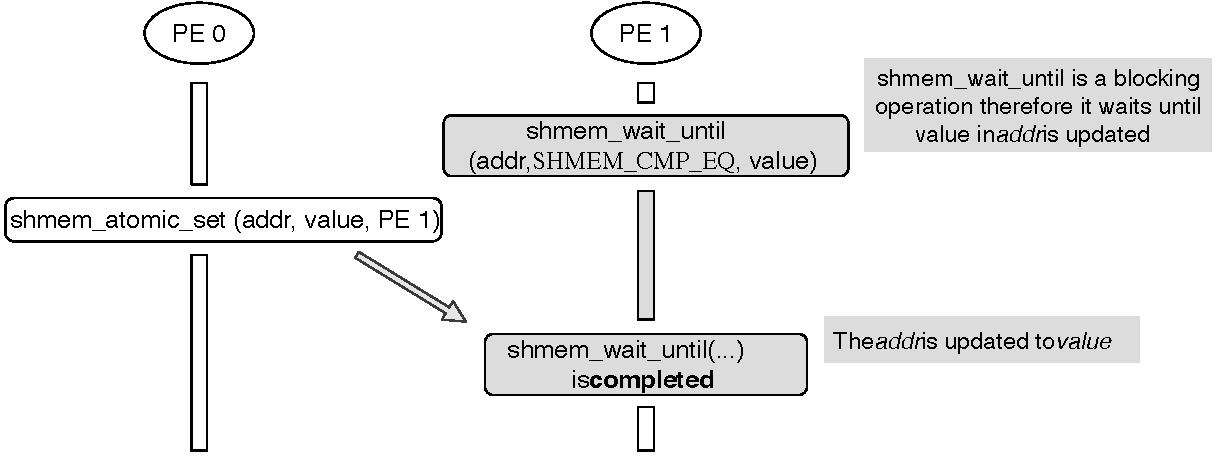
\includegraphics[width=0.7\textwidth]{figures/wait}}
\end{tabular}

\begin{tabular}{p{0.2\textwidth} | p{0.7\textwidth}}
{}
&
Waits for a symmetric variable to be updated by a remote \ac{PE}. Should be
used when computation on the local \ac{PE} cannot proceed without the value that
the remote \ac{PE} is to update. \tabularnewline
\hline 
\end{tabular}

\begin{tabular}{p{0.2\textwidth} | p{0.7\textwidth}}

{Ordering puts issued by a local \ac{PE}} \\
\FUNC{shmem\_fence} 
& 
\raisebox{-\totalheight}{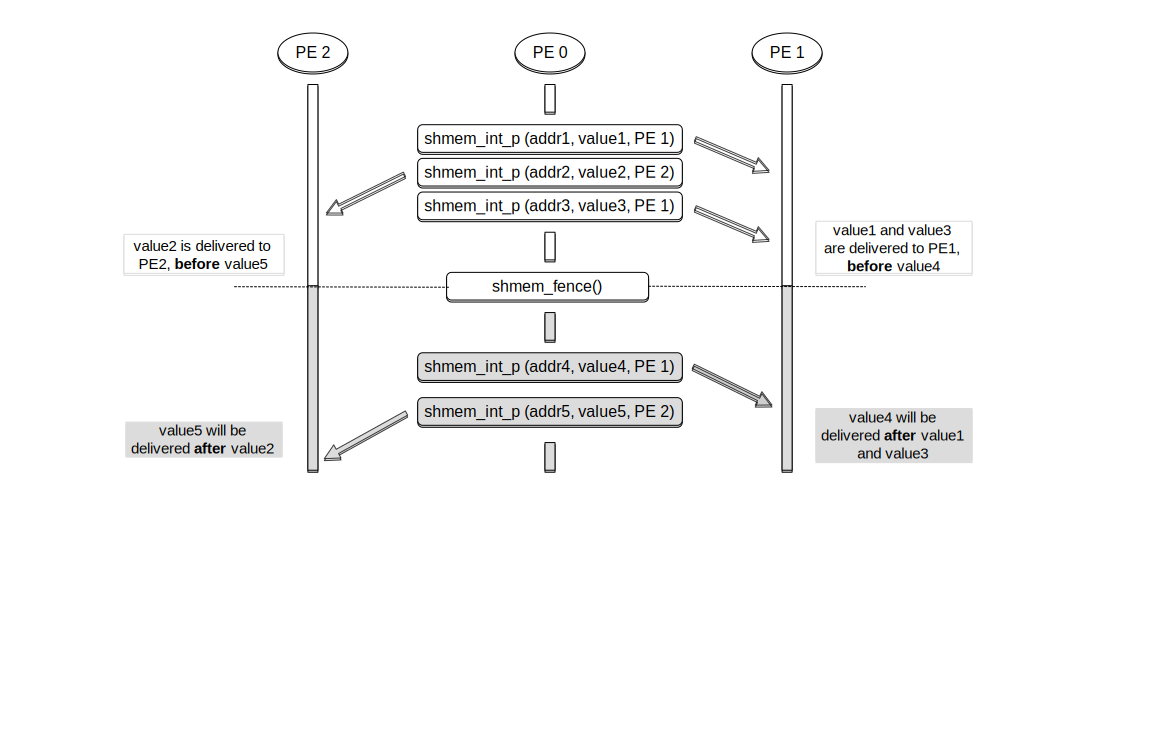
\includegraphics[width=0.7\textwidth]{figures/fence}}
\end{tabular}

\begin{tabular}{p{0.2\textwidth} | p{0.7\textwidth}}
{}
&
All \PUT{}, \acp{AMO}, store, and non-blocking \PUT{} routines on symmetric data issued to
same \ac{PE}  are guaranteed to be delivered  before Puts (to the same \ac{PE})
issued after the \FUNC{fence} call. \tabularnewline
\hline 
\end{tabular}

\begin{tabular}{p{0.2\textwidth} | p{0.7\textwidth}}
\hline 
\textbf{\openshmem  \ac{API}} & \centering \textbf{Working of \openshmem \ac{API}} \tabularnewline
\hline 
\hline
{Ordering puts issued by all \ac{PE} }\\
\FUNC{shmem\_quiet}
& 
\raisebox{-\totalheight}{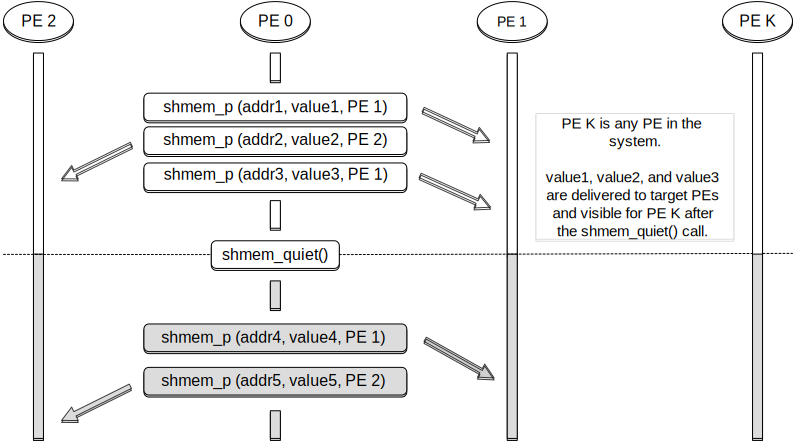
\includegraphics[width=0.7\textwidth]{figures/quiet}} 
\end{tabular}

\begin{tabular}{p{0.2\textwidth} | p{0.7\textwidth}}
{}
&
{All \PUT{}, \acp{AMO}, store, and non-blocking \PUT{} and \GET{} routines on symmetric data issued by a
local \ac{PE} to all  remote \acp{PE} are guaranteed to be completed and visible
once quiet returns. This routine should be used when all remote writes issued by
a local \ac{PE} need to be visible  to all other \acp{PE} before the local
\ac{PE} proceeds. } \tabularnewline
\hline 
\end{tabular}


\begin{tabular}{p{0.2\textwidth} | p{0.7\textwidth}}
Collective synchronization over an active set \\
\FUNC{shmem\_barrier}
&  
\raisebox{-\totalheight}{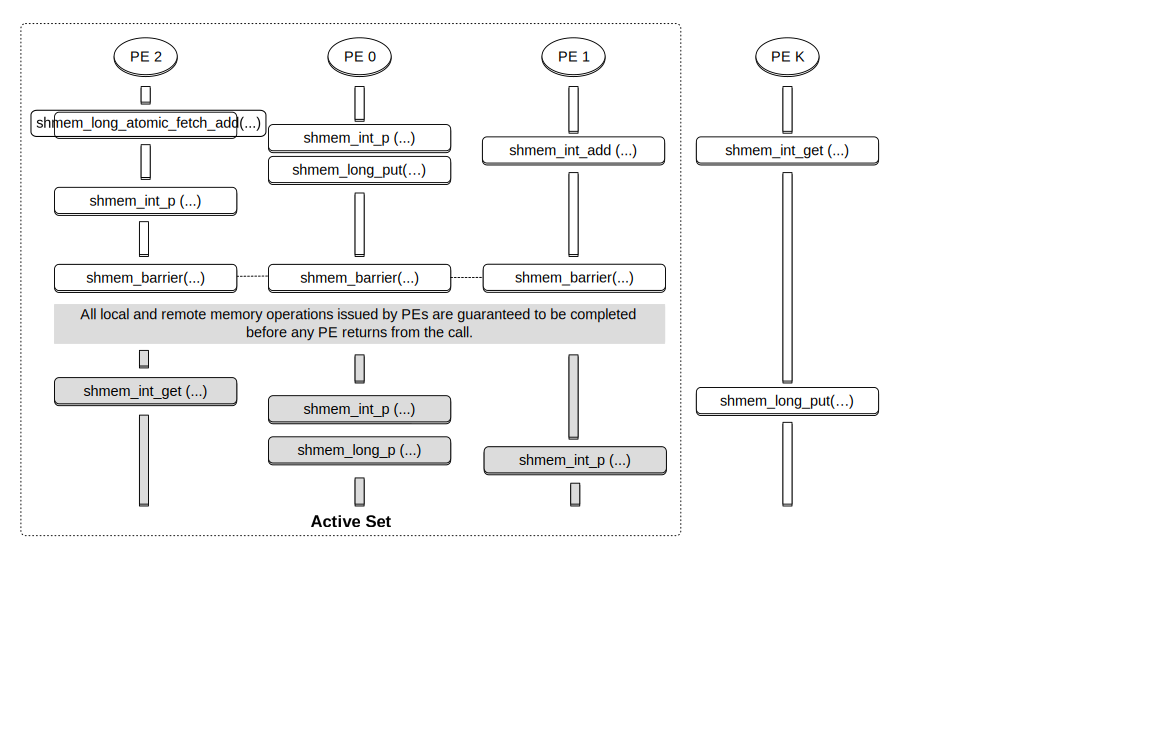
\includegraphics[width=0.7\textwidth]{figures/barrier}} 
\end{tabular}

\begin{tabular}{p{0.2\textwidth} | p{0.7\textwidth}}
{}
&
{All local and remote memory operations issued by all \acp{PE} within the
active set are guaranteed to be completed before any \ac{PE} in the
active set returns from the call. Additionally, no \ac{PE} shall return from the
barrier until all \acp{PE} in the active set have entered the same barrier
call. This routine should be used when synchronization as well as completion of
all stores and remote memory updates via \openshmem is required over a sub set
of the executing \acp{PE}.} \tabularnewline
\hline 
\end{tabular}

\begin{tabular}{p{0.2\textwidth} | p{0.7\textwidth}}
\hline 
\textbf{\openshmem  \ac{API}} & \centering \textbf{Working of \openshmem \ac{API}} \tabularnewline
\hline 
\hline
{Collective synchronization over all \acp{PE}} \\
 \FUNC{shmem\_barrier\_all}
& 
\raisebox{-\totalheight}{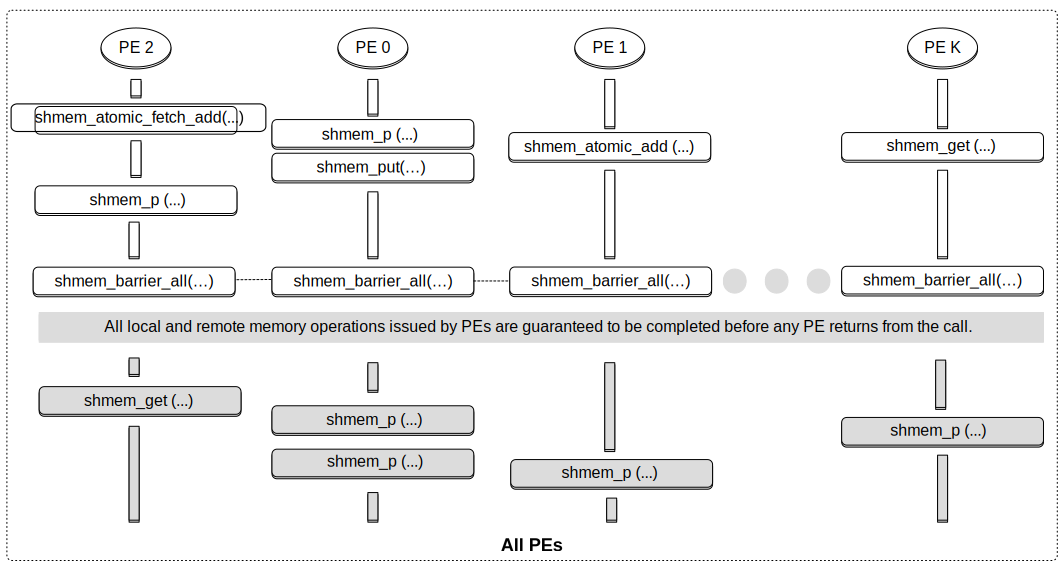
\includegraphics[width=0.7\textwidth]{figures/barrierall}}
\end{tabular}

\begin{tabular}{p{0.2\textwidth} | p{0.7\textwidth}}
{}
&
{All local and remote memory operations issued by all \acp{PE} are guaranteed to
be completed before any \ac{PE} returns from the call. Additionally no \ac{PE}
shall return from the barrier until all \acp{PE} have entered the same
\FUNC{shmem\_barrier\_all} call. This routine should be used when
synchronization as well as completion of all stores and remote memory updates
via \openshmem is required over all \acp{PE}. } \tabularnewline
\hline 
\end{tabular}
\clearpage







\subsection{Distributed Locking Routines}
The following section discusses \openshmem locks as a mechanism to provide
mutual exclusion. Three routines are available for distributed locking,
\textit{set, test} and \textit{clear}.

\subsubsection{\textbf{SHMEM\_LOCK}}\label{subsec:shmem_lock}
\apisummary{
    Releases, locks, and tests a mutual exclusion memory lock.
}
\begin{apidefinition}

\begin{Csynopsis}
void shmem_clear_lock(volatile long *lock);
void shmem_set_lock(volatile long *lock);
int shmem_test_lock(volatile long *lock);
\end{Csynopsis}

\begin{Fsynopsis}
INTEGER lock, SHMEM_TEST_LOCK
CALL SHMEM_CLEAR_LOCK(lock)
CALL SHMEM_SET_LOCK(lock)
I = SHMEM_TEST_LOCK(lock)
\end{Fsynopsis}

\begin{apiarguments}
\apiargument{IN}{lock}{A symmetric data object that is a scalar variable or an array
    of  length \CONST{1}.  This data  object  must  be set to \CONST{0} on all
    \ac{PE}s prior to the first use.  \VAR{lock}  must  be  of type \CONST{long}.
    If you are using \Fortran, it must be of default kind.}
\end{apiarguments}

\apidescription{
    The \FUNC{shmem\_set\_lock} routine sets a mutual exclusion lock after  waiting
    for  the lock  to be freed by any other \ac{PE} currently holding the lock.
    Waiting \ac{PE}s are assured of getting the lock in a first-come, first-served
    manner.  The \FUNC{shmem\_clear\_lock} routine releases a lock  previously set
    by \FUNC{shmem\_set\_lock} after ensuring that all local and remote	 stores
    initiated in the critical region are complete.  The \FUNC{shmem\_test\_lock}
    routine sets a mutual exclusion lock only if it is currently cleared.  By using
    this routine, a \ac{PE} can avoid blocking on a set lock.  If the lock is
    currently set, the routine returns without waiting.  These routines are
    appropriate for protecting a critical region from simultaneous update by
    multiple \ac{PE}s.	  
}

\apireturnvalues{
    The \FUNC{shmem\_test\_lock} routine returns \CONST{0} if  the lock  was
    originally cleared and  this  call was  able  to set the lock.  A value of
    \CONST{1} is returned if the lock had been set and the call returned without
    waiting to set the lock.
}

\apinotes{
    The term symmetric data object is defined in Section \ref{subsec:memory_model}.
    The lock variable should always be initialized to zero and accessed only by the \openshmem locking
    \ac{API}.  Changing the value of the lock variable by other means without using
    the \openshmem \ac{API}, can lead to undefined behavior.
}

\begin{apiexamples}

\apicexample
    {The following example uses \FUNC{shmem\_lock} in a \Clang{} program.}
    {./example_code/shmem_lock_example.c}
    {}

\end{apiexamples}

\end{apidefinition}






\subsection{Cache Management}
All of these routines are deprecated and are provided for backwards
compatibility.  Implementations must include all items in this section, and the
routines should function properly and may notify the user about deprecation of
their use.

\subsubsection{\textbf{SHMEM\_CACHE}}\label{subsec:shmem_cache}
\apisummary{
    Controls data cache utilities. \newtext{(This routine is deprecated and is
    provided for backwards compatibility. Implementations must include it, and
    the routines should function properly while notifying the user about
    deprecation of its use.)}
}

\begin{apidefinition}

\begin{Csynopsis}
void shmem_clear_cache_inv(void);
void shmem_set_cache_inv(void);
void shmem_clear_cache_line_inv(void *dest);
void shmem_set_cache_line_inv(void *dest);
void shmem_udcflush(void);
void shmem_udcflush_line(void *dest);
\end{Csynopsis}

\begin{Fsynopsis}
CALL SHMEM_CLEAR_CACHE_INV
CALL SHMEM_SET_CACHE_INV
CALL SHMEM_SET_CACHE_LINE_INV(dest)
CALL SHMEM_UDCFLUSH
CALL SHMEM_UDCFLUSH_LINE(dest)
\end{Fsynopsis}

\begin{apiarguments}

\apiargument{IN}{dest}{A data object that is local to the \ac{PE}.  \VAR{dest}
    can be of any noncharacter type. If you are using \Fortran, it can be of any
    kind.}

\end{apiarguments}

\apidescription{   
    \FUNC{shmem\_set\_cache\_inv} enables automatic cache coherency mode.
    
    \FUNC{shmem\_set\_cache\_line\_inv} enables automatic cache coherency mode for
    the cache line associated with the address of \VAR{dest} only.
    
    \FUNC{shmem\_clear\_cache\_inv} disables automatic cache coherency mode
    previously enabled by \FUNC{shmem\_set\_cache\ \_inv} or
    \FUNC{shmem\_set\_cache\_line\_inv}.
    
    \FUNC{shmem\_udcflush} makes the entire user data cache coherent.
    
    \FUNC{shmem\_udcflush\_line} makes coherent the cache line that corresponds with
    the address specified by \VAR{dest}.
}

\apireturnvalues{
    None.
}

\apinotes{
    These routines have been retained for improved backward compatibility with
    legacy architectures.  They are not required to be supported by implementing
    them as \VAR{no-ops} and where used, they may have no effect on cache line
    states.
}

\begin{apiexamples}

None.

\end{apiexamples}

\end{apidefinition}






\clearpage



\clearpage %%%%%%%%%%%%%%%%%%%%%%%%%%%%%%%%%%%%%%%%%%%%%%%%%%%%%%%%%%%%

\appendix

%defining pagestyle for annex
\pagestyle{fancy}
\fancyhf{}
\fancyhead[RE, LO]{\leftmark}
\fancyhead[RO, LE]{\thepage}
\fancyfoot[CE, CO]{\thepage}
\renewcommand{\headrulewidth}{0pt}




\chapter{Writing OpenSHMEM Programs}
\section*{Incorporating OpenSHMEM into Programs}\label{sec:writing_programs}

The following section describes how to write a ``Hello World" \openshmem program.
To write a ``Hello World" \openshmem program, the user must:

\begin{itemize}
\item Include the header file \HEADER{shmem.h} for \Cstd.
\item Add the initialization call \hyperref[subsec:shmem_init]{\FUNC{shmem\_init}}.
\item Use \openshmem calls to query the local \ac{PE} number
    (\hyperref[subsec:shmem_my_pe]{\FUNC{shmem\_my\_pe}}) and the total number
    of \acp{PE} (\hyperref[subsec:shmem_n_pes]{\FUNC{shmem\_n\_pes}}).
\item Add the finalization call \hyperref[subsec:shmem_finalize]{\FUNC{shmem\_finalize}}.
\end{itemize}

In \openshmem, the order in which lines appear in the output is not
deterministic because \acp{PE} execute asynchronously in parallel.

\SourceExample{example_code/hello-openshmem.c}{
  \label{openshmem-hello}
  ``Hello World'' example program in \Cstd
}

\ProgramOutput{example_code/hello-openshmem-c.output}{
  Possible ordering of expected output with 4 \acp{PE} from the
  program in Example~\ref{openshmem-hello}
}

\clearpage %%%%%%%%%%%%%%%%%%%%%%%%%%%%%%%%%%%%%%%%%%%%%%%%%%%%%%%%%%%%

Example~\ref{openshmem-hello-symmetric} shows a more complex
\openshmem program that illustrates the use of symmetric data objects.
Note the declaration of the \VAR{static short dest} array and its use as the
remote destination in \hyperref[subsec:shmem_put]{\FUNC{shmem\_put}}.

The \KEYWORD{static} keyword makes the \VAR{dest} array symmetric on all \acp{PE}.
Each \ac{PE} is able to transfer data to a remote \dest{} array by simply
specifying to an OpenSHMEM routine such as \hyperref[subsec:shmem_put]{\FUNC{shmem\_put}}
the local address of the symmetric data object that will receive the data.
This local address resolution aids programmability because the address of the
\dest{} need not be exchanged with the active side (\ac{PE} \CONST{0}) prior to
the \acf{RMA} routine.

Conversely, the declaration of the \VAR{short source} array is asymmetric
(local only).
The \source{} object does not need to be symmetric because \PUT{} handles the
references to the \VAR{source} array only on the active (local) side.

\SourceExample{example_code/writing_shmem_example.c}{
  \label{openshmem-hello-symmetric}
  Example program with symmetric data objects
}

\ProgramOutput{example_code/writing_shmem_example.output}{
  Possible ordering of expected output with 4~\acp{PE} from the
  program in Example~\ref{openshmem-hello-symmetric}
}

\chapter{Compiling and Running Programs}\label{sec:compiling}
The \openshmem Specification does not specify how
\openshmem programs are compiled, linked, and run. This section shows some
examples of how wrapper programs are utilized in the \openshmem Reference
Implementation to compile and launch programs.

\section{Compilation}
\subsection*{Programs written in \Cstd}

The \openshmem Reference Implementation provides a wrapper program, named
\textbf{oshcc}, to aid in the compilation of \Cstd programs.
The wrapper may be called as follows:

\begin{lstlisting}[]
oshcc <compiler options> -o myprogram myprogram.c
\end{lstlisting}
Where the $\langle\mbox{compiler options}\rangle$ are options understood by the
underlying \Cstd compiler called by \textbf{oshcc}.


\subsection*{Programs written in \Cpp}

The \openshmem Reference Implementation provides a wrapper program, named
\textbf{oshc++}, to aid in the compilation of \Cpp programs.
The wrapper may be called as follows:

\begin{lstlisting}[]
oshc++ <compiler options> -o myprogram myprogram.cpp
\end{lstlisting}
Where the $\langle\mbox{compiler options}\rangle$ are options understood by the
underlying \Cpp compiler called by \textbf{oshc++}.


\section{Running Programs}

The \openshmem Reference Implementation provides a wrapper program, named
\textbf{oshrun}, to launch \openshmem programs.
The wrapper may be called as follows:

\begin{lstlisting}[]
oshrun <runner options> -np <#> <program> <program arguments>
\end{lstlisting}
The arguments for \textbf{oshrun} are:

\begin{tabular}{p{0.3\textwidth}p{0.6\textwidth}}
$\langle\mbox{runner options}\rangle$ & {Options passed to the underlying launcher.}\tabularnewline
-np $\langle\mbox{\#}\rangle$ & {The number of \acp{PE} to be used in the execution.}\tabularnewline
$\langle\mbox{program}\rangle$ & {The program executable to be launched.}\tabularnewline
$\langle\mbox{program arguments}\rangle$ & {Flags and other parameters to pass to the program.}\tabularnewline
\end{tabular}




\chapter{Undefined Behavior in OpenSHMEM}\label{sec:undefined}

The \openshmem Specification formalizes the expected behavior of
its library routines.  In cases where routines are improperly used
or the input is not in accordance with the Specification, the behavior
is undefined.

\begin{longtable}{|>{\raggedright}p{0.3\textwidth}|>{\raggedright}p{0.6\textwidth}|}
\hline
\textbf{Inappropriate Usage} & \textbf{Undefined Behavior}\tabularnewline
\hline
\endhead
Uninitialized library & If the \openshmem library is not initialized,
calls to non-initializing \openshmem routines have undefined
behavior.  For example, an implementation may try to continue or may abort
immediately upon an \openshmem call into the uninitialized library.
\tabularnewline
\hline
Multiple calls to initialization routines & In an \openshmem program where
the initialization routines \FUNC{shmem\_init} or \FUNC{shmem\_init\_thread}
have already been called, any subsequent calls to these initialization routines
result in undefined behavior.
\tabularnewline
\hline
Specifying invalid \ac{PE} numbers & For \openshmem routines that accept a
\ac{PE} number as an argument, if the \ac{PE} number is invalid for the
team associated with the operation (either implicitly or explicitly), the
behavior is undefined.  An invalid \ac{PE} number includes those that are
negative or greater than or equal to the size of the associated team.
\tabularnewline
\hline
Use of non-symmetric variables & Some routines require remotely accessible
variables to perform their function.  For example, a \PUT{} to a non-symmetric variable may
be trapped where possible and the library may abort the program.  Another
implementation may choose to continue execution with or without a warning.
\tabularnewline
\hline
Non-symmetric allocation of symmetric memory & The symmetric memory management routines are
collectives. For example, all \acp{PE} in the program must call
\FUNC{shmem\_malloc} with the same \VAR{size} argument.  Program behavior after a
mismatched \FUNC{shmem\_malloc} call is undefined.\tabularnewline
\hline
Use of null pointers with non-zero \VAR{len} specified & In any \openshmem routine
that takes a pointer and \VAR{len} describing the number of elements in that
pointer, a null pointer may not be given unless the corresponding \VAR{len} is also
specified as zero. Otherwise, the resulting behavior is undefined.
The following cases summarize this behavior:
\begin{itemize}
    \item \VAR{len} is 0, pointer is null: supported.
    \item \VAR{len} is not 0, pointer is null: undefined behavior.
    \item \VAR{len} is 0, pointer is non-null: supported.
    \item \VAR{len} is not 0, pointer is non-null: supported.
\end{itemize}
\tabularnewline
\hline
Concurrent use of a team & Teams are not thread-safe objects.
Concurrent use of a team from multiple threads results in undefined
behavior.  Such a situation can arise when one thread is calling a
team-implicit collective (e.g., \FUNC{shmem\_barrier\_all}), which
implicitly operates on the world team, and another calls a team-based
collective (e.g., \FUNC{shmem\_broadcastmem}). \tabularnewline
\hline
Destroying a team with unfreed private contexts & Before destroying a given
team, the user is responsible for destroying all contexts created from that team
with the \LibConstRef{SHMEM\_CTX\_PRIVATE} option enabled; otherwise, the
behavior is undefined.\tabularnewline
\hline
\end{longtable}


\chapter{Interoperability with Other Programming Models}\label{sec:interoperability}

OpenSHMEM routines may be used in conjunction with the routines of other
communication libraries or parallel languages in the same program. This section
describes the interoperability with other programming models, including
clarification of undefined behaviors caused by mixed use of different models,
and advice to \openshmem library users and developers that may improve the portability
and performance of hybrid programs.


\section{\ac{MPI} Interoperability}

\openshmem and \ac{MPI} are two commonly used parallel programming models for
distributed-memory systems. The user can choose to utilize both models in the same program
to efficiently and easily support various communication patterns.

A vendor may implement the \openshmem and \ac{MPI} libraries in different ways. For
instance, one may implement both \openshmem and \ac{MPI} as standalone libraries,
each of which allocates and initializes fully isolated communication
resources.
Another approach
is to implement both \openshmem and \ac{MPI} interfaces within the
same software system in order to share a communication resource when possible.

To improve interoperability and portability in \openshmem + \ac{MPI} hybrid
programming, we clarify the relevant semantics in the following subsections.


\subsection{Initialization}
In order to ensure that a hybrid program can be portably performed with different vendor
implementations, the \openshmem environment of the program must be initialized by
a call to \FUNC{shmem\_init} or \FUNC{shmem\_init\_thread} and be finalized by
a call to \FUNC{shmem\_finalize}; the \ac{MPI} environment of the program must be initialized
by a call to \FUNC{MPI\_Init} or \FUNC{MPI\_Init\_thread} and be finalized by a
call to \FUNC{MPI\_Finalize}.

\apiimpnotes{
Portable implementations of OpenSHMEM and \ac{MPI} must ensure that the initialization
calls can be made in an arbitrary order within a program; the same rule also
applies to the finalization calls. A software runtime that utilizes a shared
communication resource for \openshmem and \ac{MPI} communication may maintain an
internal reference counter in order to ensure that the shared resource is
initialized only once and thus no shared resource is released until the last
finalization call is made.
}


\subsection{Dynamic Process Creation}
\label{subsec:interoperability:mpmd}

\ac{MPI} defines a dynamic process model that allows creation of processes after
an \ac{MPI} application has started (e.g., by calling \FUNC{MPI\_Comm\_spawn}) and
connection to independent processes (e.g., through \FUNC{MPI\_Comm\_accept}
and \FUNC{MPI\_Comm\_connect}).
It provides a mechanism to establish communication
between the newly created processes and the existing \ac{MPI} application (see
\ac{MPI} standard version 3.1, Chapter 10).
Unlike \ac{MPI}, \openshmem starts all processes at once and requires all \acp{PE} to
collectively allocate and initialize resources (e.g., symmetric heap) used by
the \openshmem library before any other \openshmem routine may
be called. \openshmem does not support communication with dynamically created
or connected processes. In such a scenario, \ac{MPI} can be used to communicate
with these processes.


\subsection{Thread Safety}
\label{subsec:interoperability:thread}
Both \openshmem and \ac{MPI} define the interaction with user threads in a program
with routines that can be used for initializing and querying the thread
environment. A hybrid program may request different thread levels
at the initialization calls of \openshmem and \ac{MPI} environments; however, the
returned support level provided by the \openshmem or \ac{MPI} library might be different
from that returned in an non-hybrid program. For instance, the former
initialization call in a hybrid program may initialize a resource with the
requested thread level, but the supported level cannot be updated by a subsequent
initialization call if the underlying software runtime of \openshmem and \ac{MPI}
share the same internal communication resource.
The program should always check the \VAR{provided} thread level returned
at the corresponding initialization call or query the level of thread support
after initialization to portably ensure thread support in each communication
environment.

Both \openshmem and \ac{MPI} define similar thread levels, namely, \VAR{THREAD\_SINGLE},
\VAR{THREAD\_FUNNELED}, \VAR{THREAD\_SERIALIZED}, and \VAR{THREAD\_MULTIPLE}.
When requesting threading support in a hybrid program, however,
the following additional rules are applied if the implementations of \openshmem
and \ac{MPI} share the same internal communication resource.
It is strongly recommended to always follow these rules to ensure program
portability.

\begin{itemize}
    \item The \VAR{THREAD\_SINGLE} thread level requires a single-threaded program.
    Hence, a hybrid program should not request \VAR{THREAD\_SINGLE} at the initialization
    call of either \openshmem or \ac{MPI} but request a different thread level at the
    initialization call of the other model.

    \item The \VAR{THREAD\_FUNNELED} thread level allows only the main thread to
    make communication calls. A hybrid program using the \VAR{THREAD\_FUNNELED}
    thread level in both \openshmem and \ac{MPI} should ensure that the same main thread
    is used in both communication environments.

    \item The \VAR{THREAD\_SERIALIZED} thread level requires the program to ensure
    that communication calls are not made concurrently by multiple threads. If a
    hybrid program uses \VAR{THREAD\_SERIALIZED} in one communication environment
    and \VAR{THREAD\_SERIALIZED} or \VAR{THREAD\_FUNNELED} in the other one, it
    should also guarantee that the \openshmem and \ac{MPI} calls are not made concurrently
    from two distinct threads.
\end{itemize}

\subsection{Mapping Process Identification Numbers}
\label{subsec:interoperability:id}

Similar to the \ac{PE} number in \openshmem, \ac{MPI} defines rank as the
identification number of a process in a communicator. Both the \openshmem \ac{PE}
and the \ac{MPI} rank are unique integers assigned from zero to one less than the total
number of processes. In a hybrid program, the \openshmem
\ac{PE} number in \LibHandleRef{SHMEM\_TEAM\_WORLD}
and the \ac{MPI} rank in \VAR{MPI\_COMM\_WORLD} of a process can be equal.
This feature, however, may be provided by only some of the \openshmem and \ac{MPI}
implementations (e.g., if both environments share the same underlying process
manager) and is not portably guaranteed. A portable program should always
use the standard functions in each model, namely, \FUNC{shmem\_team\_my\_pe} in \openshmem
and \FUNC{MPI\_Comm\_rank} in \ac{MPI}, to query the process identification numbers
in each communication environment and manage the mapping of identifiers in the
program when necessary.

\subsubsection*{Examples}
\label{subsubsec:interoperability:id:example}
The following example demonstrates how to manage the mapping between \openshmem
\ac{PE} numbers and \ac{MPI} ranks in \VAR{MPI\_COMM\_WORLD} in a hybrid \openshmem
and \ac{MPI} program.

\lstinputlisting[language={C}, tabsize=2,
      basicstyle=\ttfamily\footnotesize]
      {example_code/hybrid_mpi_mapping_id.c}

The following example demonstrates an alternative approach for managing the mapping
of process identification numbers in a hybrid program. The program creates a
new MPI communicator, named \VAR{shmem\_comm}, that contains all
processes in \VAR{MPI\_COMM\_WORLD} and uses the same \ac{MPI} rank and
\openshmem \ac{PE} numbering.

\lstinputlisting[language={C}, tabsize=2,
      basicstyle=\ttfamily\footnotesize]
      {example_code/hybrid_mpi_mapping_id_shmem_comm.c}

\subsection{RMA Programming Models}
\label{subsec:interoperability:rma}

\openshmem and \ac{MPI} each define similar one-sided communication models;
however, a portable program should not assume interoperability between these
models.
For instance, \openshmem guarantees the atomicity only of concurrent \openshmem AMO operations
that operate on symmetric data with the same datatype. Access to the same symmetric
object with \ac{MPI} atomic operations, such as an \FUNC{MPI\_Fetch\_and\_op}, may
result in an undefined result. A hybrid program should avoid situations where \ac{MPI} and
\openshmem one-sided operations perform concurrent accesses to the same memory
location; otherwise, the behavior is undefined.

\subsection{Communication Progress}
\label{subsec:interoperability:progress}

\openshmem promises the progression of communication both with and without
\openshmem calls and requires the software progress mechanism in the implementation
(e.g., a progress thread) when the hardware does not provide asynchronous communication
capabilities (see Section \ref{subsec:progress}).
In \ac{MPI}, however, a weak progress semantics is applied. That is,
an \ac{MPI} communication call is guaranteed only to complete in finite time. For
instance, an \FUNC{MPI\_Put} may be completed only when the remote process makes an \ac{MPI}
call that internally triggers the progress of \ac{MPI}, if the underlying hardware
does not support asynchronous communication. A hybrid program
should not assume that the \openshmem library also makes progress for \ac{MPI}.
It can explicitly manage the asynchronous communication of \ac{MPI} in
order to prevent any deadlock or performance degradation.


\chapter{History of OpenSHMEM}\label{sec:openshmem_history}

SHMEM has a long history as a parallel-programming model and has been
extensively used on a number of products since 1993, including the Cray T3D,
Cray X1E, Cray XT3 and XT4, \ac{SGI} Origin, \ac{SGI} Altix, Quadrics-based
clusters, and InfiniBand-based clusters.

\begin{itemize}
\item SHMEM Timeline
  \begin{itemize}
  \item Cray SHMEM
    \begin{itemize}
    \item SHMEM first introduced by Cray Research, Inc.\ in 1993 for Cray T3D
    \item Cray was acquired by \ac{SGI} in 1996
    \item Cray was acquired by Tera in 2000 (MTA)
    \item Platforms: Cray T3D, T3E, C90, J90, SV1, SV2, X1, X2, XE, XMT, XT
    \end{itemize}
  \item \ac{SGI} SHMEM
    \begin{itemize}
    \item \ac{SGI} acquired Cray Research, Inc.\ and SHMEM was integrated into
      \ac{SGI}'s Message Passing Toolkit (MPT)
    \item \ac{SGI} currently owns the rights to SHMEM and \openshmem
    \item Platforms: Origin, Altix 4700, Altix XE, ICE, UV
    \item \ac{SGI} was acquired by Rackable Systems in 2009
    \item \ac{SGI} and \ac{OSSS} signed a
      SHMEM trademark licensing agreement in 2010
    \item \ac{HPE} acquired {SGI} in 2016
    \end{itemize}
  \end{itemize}
\end{itemize}

A listing of \openshmem implementations can be found on
\url{http://www.openshmem.org/}.








\chapter{OpenSHMEM Specification and Deprecated API}\label{sec:dep_api}

\section{Overview}\label{subsec:dep_overview}
\TableIndex{Deprecated API}
For the \openshmem Specification, deprecation is the process of identifying
API that is supported but no longer recommended for use by users.
The deprecated API \textbf{must} be supported until clearly
indicated as otherwise by the Specification.
This chapter records the API or functionality that have been deprecated, the
version of the \openshmem Specification that effected the deprecation, and the
most recent version of the \openshmem Specification in which the feature was
supported before removal.

\begin{center}
\scriptsize
\begin{longtable}{|l|c|c|l|}
    \hline
    \textbf{Deprecated API}
    & \textbf{Deprecated Since}
    & \textbf{Last Version Supported}
    & \textbf{Replaced By} \\
    \hline
    \endhead
    %% Deprecated in 1.1
    Header Directory: \hyperref[subsec:dep_rationale:mpp]{\HEADER{mpp}} & 1.1 & Current & (none) \\ \hline
    %% Deprecated in 1.2
    \CorCpp: \hyperref[subsec:start_pes]{\FuncRef{start\_pes}} & 1.2 & Current & \hyperref[subsec:shmem_init]{\FUNC{shmem\_init}} \\ \hline
    \Fortran: \hyperref[subsec:start_pes]{\FuncRef{START\_PES}} & 1.2 & 1.4 & \hyperref[subsec:shmem_init]{\FUNC{SHMEM\_INIT}} \\ \hline
    \hyperref[subsec:start_pes]{Implicit finalization} & 1.2 & Current & \hyperref[subsec:shmem_finalize]{\FUNC{shmem\_finalize}} \\ \hline
    \CorCpp: \FuncRef{\_my\_pe} & 1.2 & Current & \hyperref[subsec:shmem_my_pe]{\FUNC{shmem\_my\_pe}} \\ \hline
    \CorCpp: \FuncRef{\_num\_pes} & 1.2 & Current & \hyperref[subsec:shmem_n_pes]{\FUNC{shmem\_n\_pes}} \\ \hline
    \Fortran: \FuncRef{MY\_PE} & 1.2 & 1.4 & \hyperref[subsec:shmem_my_pe]{\FUNC{SHMEM\_MY\_PE}} \\ \hline
    \Fortran: \FuncRef{NUM\_PES} & 1.2 & 1.4 & \hyperref[subsec:shmem_n_pes]{\FUNC{SHMEM\_N\_PES}} \\ \hline
    \CorCpp: \FuncRef{shmalloc} & 1.2 & Current & \hyperref[subsec:shfree]{\FUNC{shmem\_malloc}} \\ \hline
    \CorCpp: \FuncRef{shfree} & 1.2 & Current & \hyperref[subsec:shfree]{\FUNC{shmem\_free}} \\ \hline
    \CorCpp: \FuncRef{shrealloc} & 1.2 & Current & \hyperref[subsec:shfree]{\FUNC{shmem\_realloc}} \\ \hline
    \CorCpp: \FuncRef{shmemalign} & 1.2 & Current & \hyperref[subsec:shfree]{\FUNC{shmem\_align}} \\ \hline
    \Fortran: \FuncRef{SHMEM\_PUT} & 1.2 & 1.4 & \hyperref[subsec:shmem_put]{\FUNC{SHMEM\_PUT8} or \FUNC{SHMEM\_PUT64}} \\ \hline
    %% Deprecated in 1.3
    \minitab{
        \CorCpp: \FuncRef{shmem\_clear\_cache\_inv}
        \\ \CorCpp: \FuncRef{shmem\_clear\_cache\_line\_inv}
        \\ \CorCpp: \FuncRef{shmem\_set\_cache\_inv}
        \\ \CorCpp: \FuncRef{shmem\_set\_cache\_line\_inv}
        \\ \CorCpp: \FuncRef{shmem\_udcflush}
        \\ \CorCpp: \FuncRef{shmem\_udcflush\_line}
        } & 1.3 & 1.4 & (none) \\ \hline
    \minitab{
        \Fortran: \FuncRef{SHMEM\_CLEAR\_CACHE\_INV}
        %% Note: At the time of deprecation, the Fortran API did not specify
        %% SHMEM_CLEAR_CACHE_LINE_INV. While this omission is certainly an error,
        %% Fortran was removed in 1.5 so the omission was never corrected.
        \\ \Fortran: \FuncRef{SHMEM\_SET\_CACHE\_INV}
        \\ \Fortran: \FuncRef{SHMEM\_SET\_CACHE\_LINE\_INV}
        \\ \Fortran: \FuncRef{SHMEM\_UDCFLUSH}
        \\ \Fortran: \FuncRef{SHMEM\_UDCFLUSH\_LINE}
        } & 1.3 & 1.4 & (none) \\ \hline
    \LibConstRef{\_SHMEM\_SYNC\_VALUE}         & 1.3 & Current & \hyperref[subsec:library_constants]{\CONST{SHMEM\_SYNC\_VALUE}} \\ \hline
    \LibConstRef{\_SHMEM\_BARRIER\_SYNC\_SIZE} & 1.3 & Current & \hyperref[subsec:library_constants]{\CONST{SHMEM\_BARRIER\_SYNC\_SIZE}} \\ \hline
    \LibConstRef{\_SHMEM\_BCAST\_SYNC\_SIZE}   & 1.3 & Current & \hyperref[subsec:library_constants]{\CONST{SHMEM\_BCAST\_SYNC\_SIZE}} \\ \hline
    \LibConstRef{\_SHMEM\_COLLECT\_SYNC\_SIZE} & 1.3 & Current & \hyperref[subsec:library_constants]{\CONST{SHMEM\_COLLECT\_SYNC\_SIZE}} \\ \hline
    \LibConstRef{\_SHMEM\_REDUCE\_SYNC\_SIZE}  & 1.3 & Current & \hyperref[subsec:library_constants]{\CONST{SHMEM\_REDUCE\_SYNC\_SIZE}} \\ \hline
    \LibConstRef{\_SHMEM\_REDUCE\_MIN\_WRKDATA\_SIZE} & 1.3 & Current & \hyperref[subsec:library_constants]{\CONST{SHMEM\_REDUCE\_MIN\_WRKDATA\_SIZE}} \\ \hline
    \LibConstRef{\_SHMEM\_MAJOR\_VERSION} & 1.3 & Current & \hyperref[subsec:library_constants]{\CONST{SHMEM\_MAJOR\_VERSION}} \\ \hline
    \LibConstRef{\_SHMEM\_MINOR\_VERSION} & 1.3 & Current & \hyperref[subsec:library_constants]{\CONST{SHMEM\_MINOR\_VERSION}} \\ \hline
    \LibConstRef{\_SHMEM\_MAX\_NAME\_LEN} & 1.3 & Current & \hyperref[subsec:library_constants]{\CONST{SHMEM\_MAX\_NAME\_LEN}} \\ \hline
    \LibConstRef{\_SHMEM\_VENDOR\_STRING} & 1.3 & Current & \hyperref[subsec:library_constants]{\CONST{SHMEM\_VENDOR\_STRING}} \\ \hline
    \LibConstRef{\_SHMEM\_CMP\_EQ} & 1.3 & Current & \hyperref[subsec:library_constants]{\CONST{SHMEM\_CMP\_EQ}} \\ \hline
    \LibConstRef{\_SHMEM\_CMP\_NE} & 1.3 & Current & \hyperref[subsec:library_constants]{\CONST{SHMEM\_CMP\_NE}} \\ \hline
    \LibConstRef{\_SHMEM\_CMP\_LT} & 1.3 & Current & \hyperref[subsec:library_constants]{\CONST{SHMEM\_CMP\_LT}} \\ \hline
    \LibConstRef{\_SHMEM\_CMP\_LE} & 1.3 & Current & \hyperref[subsec:library_constants]{\CONST{SHMEM\_CMP\_LE}} \\ \hline
    \LibConstRef{\_SHMEM\_CMP\_GT} & 1.3 & Current & \hyperref[subsec:library_constants]{\CONST{SHMEM\_CMP\_GT}} \\ \hline
    \LibConstRef{\_SHMEM\_CMP\_GE} & 1.3 & Current & \hyperref[subsec:library_constants]{\CONST{SHMEM\_CMP\_GE}} \\ \hline
    %% Deprecated in 1.4
    \EnvVarRef{SMA\_VERSION}         & 1.4 & Current & \hyperref[subsec:environment_variables]{\ENVVAR{SHMEM\_VERSION}} \\ \hline
    \EnvVarRef{SMA\_INFO}            & 1.4 & Current & \hyperref[subsec:environment_variables]{\ENVVAR{SHMEM\_INFO}} \\ \hline
    \EnvVarRef{SMA\_SYMMETRIC\_SIZE} & 1.4 & Current & \hyperref[subsec:environment_variables]{\ENVVAR{SHMEM\_SYMMETRIC\_SIZE}} \\ \hline
    \EnvVarRef{SMA\_DEBUG}           & 1.4 & Current & \hyperref[subsec:environment_variables]{\ENVVAR{SHMEM\_DEBUG}} \\ \hline
    \minitab{\CorCpp: \FuncRef{shmem\_wait}
        \\ \CorCpp: \FuncRef{shmem\_\FuncParam{TYPENAME}\_wait}}
        & 1.4 & Current & See \textbf{Notes} for \hyperref[subsec:shmem_wait_until]{\FUNC{shmem\_wait\_until}} \\ \hline
    \CorCpp: \FuncRef{shmem\_wait\_until} & 1.4 & Current
        & \Cstd[11]: \hyperref[subsec:shmem_wait_until]{\FUNC{shmem\_wait\_until}}, \CorCpp: \hyperref[subsec:shmem_wait_until]{\FUNC{shmem\_long\_wait\_until}} \\ \hline
    \minitab{\Cstd[11]: \FuncRef{shmem\_fetch}
        \\ \CorCpp: \FuncRef{shmem\_\FuncParam{TYPENAME}\_fetch}}
        & 1.4 & Current & \hyperref[subsec:shmem_atomic_fetch]{\FUNC{shmem\_atomic\_fetch}} \\ \hline
    \minitab{\Cstd[11]: \FuncRef{shmem\_set}
        \\ \CorCpp: \FuncRef{shmem\_\FuncParam{TYPENAME}\_set}}
        & 1.4 & Current & \hyperref[subsec:shmem_atomic_set]{\FUNC{shmem\_atomic\_set}} \\ \hline
    \minitab{\Cstd[11]: \FuncRef{shmem\_cswap}
        \\ \CorCpp: \FuncRef{shmem\_\FuncParam{TYPENAME}\_cswap}}
        & 1.4 & Current & \hyperref[subsec:shmem_atomic_compare_swap]{\FUNC{shmem\_atomic\_compare\_swap}} \\ \hline
    \minitab{\Cstd[11]: \FuncRef{shmem\_swap}
        \\ \CorCpp: \FuncRef{shmem\_\FuncParam{TYPENAME}\_swap}}
        & 1.4 & Current & \hyperref[subsec:shmem_atomic_swap]{\FUNC{shmem\_atomic\_swap}} \\ \hline
    \minitab{\Cstd[11]: \FuncRef{shmem\_finc}
        \\ \CorCpp: \FuncRef{shmem\_\FuncParam{TYPENAME}\_finc}}
        & 1.4 & Current & \hyperref[subsec:shmem_atomic_fetch_inc]{\FUNC{shmem\_atomic\_fetch\_inc}} \\ \hline
    \minitab{\Cstd[11]: \FuncRef{shmem\_inc}
        \\ \CorCpp: \FuncRef{shmem\_\FuncParam{TYPENAME}\_inc}}
        & 1.4 & Current & \hyperref[subsec:shmem_atomic_inc]{\FUNC{shmem\_atomic\_inc}} \\ \hline
    \minitab{\Cstd[11]: \FuncRef{shmem\_fadd}
        \\ \CorCpp: \FuncRef{shmem\_\FuncParam{TYPENAME}\_fadd}}
        & 1.4 & Current & \hyperref[subsec:shmem_atomic_fetch_add]{\FUNC{shmem\_atomic\_fetch\_add}} \\ \hline
    \minitab{\Cstd[11]: \FuncRef{shmem\_add}
        \\ \CorCpp: \FuncRef{shmem\_\FuncParam{TYPENAME}\_add}}
        & 1.4 & Current & \hyperref[subsec:shmem_atomic_add]{\FUNC{shmem\_atomic\_add}} \\ \hline
    Entire \Fortran API & 1.4 & 1.4 & \openshmem \Cstd API through \Fortran--\Cstd interoperability \\ \hline
    %% Deprecated in 1.5
    \minitab{
        \LibConstRef{SHMEM\_SYNC\_VALUE}
        \\ \LibConstRef{SHMEM\_SYNC\_SIZE}
        \\ \LibConstRef{SHMEM\_BARRIER\_SYNC\_SIZE}
        \\ \LibConstRef{SHMEM\_ALLTOALL\_SYNC\_SIZE}
        \\ \LibConstRef{SHMEM\_ALLTOALLS\_SYNC\_SIZE}
        \\ \LibConstRef{SHMEM\_BCAST\_SYNC\_SIZE}
        \\ \LibConstRef{SHMEM\_COLLECT\_SYNC\_SIZE}
        \\ \LibConstRef{SHMEM\_REDUCE\_SYNC\_SIZE}
        \\ \LibConstRef{SHMEM\_REDUCE\_MIN\_WRKDATA\_SIZE}
    } & 1.5 & Current & Team-based collectives, \minitab{Section~\ref{subsec:team_collectives}}. \\ \hline
    \CorCpp: Active-set-based \FuncRef{shmem\_sync}
        & 1.5 & Current & Team-based \hyperref[subsec:shmem_sync]{\FUNC{shmem\_sync}} \\ \hline
    \CorCpp: \FuncRef{shmem\_alltoall[32,64]} & 1.5 & Current &
    \hyperref[subsec:shmem_alltoall]{\FUNC{shmem\_alltoall}} \\ \hline
    \CorCpp: \FuncRef{shmem\_alltoalls[32,64]} & 1.5 & Current &
    \hyperref[subsec:shmem_alltoalls]{\FUNC{shmem\_alltoalls}} \\ \hline
    \CorCpp: \FuncRef{shmem\_broadcast[32,64]} & 1.5 & Current &
    \hyperref[subsec:shmem_broadcast]{\FUNC{shmem\_broadcast}} \\ \hline
    \CorCpp: \FuncRef{shmem\_collect[32,64]} & 1.5 & Current &
    \hyperref[subsec:shmem_collect]{\FUNC{shmem\_collect}} \\ \hline
    \CorCpp: \FuncRef{shmem\_fcollect[32,64]} & 1.5 & Current &
    \hyperref[subsec:shmem_collect]{\FUNC{shmem\_fcollect}} \\ \hline
    \CorCpp: \FuncRef{shmem\_\FuncParam{TYPENAME}\_and\_to\_all}
        & 1.5 & Current & \hyperref[subsec:shmem_and_reduce]{\FUNC{shmem\_and\_reduce}} \\ \hline
    \CorCpp: \FuncRef{shmem\_\FuncParam{TYPENAME}\_or\_to\_all}
        & 1.5 & Current & \hyperref[subsec:shmem_or_reduce]{\FUNC{shmem\_or\_reduce}} \\ \hline
    \CorCpp: \FuncRef{shmem\_\FuncParam{TYPENAME}\_xor\_to\_all}
        & 1.5 & Current & \hyperref[subsec:shmem_xor_reduce]{\FUNC{shmem\_xor\_reduce}} \\ \hline
    \CorCpp: \FuncRef{shmem\_\FuncParam{TYPENAME}\_max\_to\_all}
        & 1.5 & Current & \hyperref[subsec:shmem_max_reduce]{\FUNC{shmem\_max\_reduce}} \\ \hline
    \CorCpp: \FuncRef{shmem\_\FuncParam{TYPENAME}\_min\_to\_all}
        & 1.5 & Current & \hyperref[subsec:shmem_min_reduce]{\FUNC{shmem\_min\_reduce}} \\ \hline
    \CorCpp: \FuncRef{shmem\_\FuncParam{TYPENAME}\_sum\_to\_all}
        & 1.5 & Current & \hyperref[subsec:shmem_sum_reduce]{\FUNC{shmem\_sum\_reduce}} \\ \hline
    \CorCpp: \FuncRef{shmem\_\FuncParam{TYPENAME}\_prod\_to\_all}
        & 1.5 & Current & \hyperref[subsec:shmem_prod_reduce]{\FUNC{shmem\_prod\_reduce}} \\ \hline
    \CorCpp: \hyperref[subsec:shmem_barrier]{\FuncRef{shmem\_barrier}}
        & 1.5 & Current & \hyperref[subsec:shmem_quiet]{\FuncRef{shmem\_quiet}} + \hyperref[subsec:shmem_sync]{\FuncRef{shmem\_sync}} \\ \hline
    %% Deprecated in 1.6
    %% Deprecated in 1.7
    %% Notes
    %% - If a hyperref spans more than one line vertically, the clickable box
    %%   will also span more than one line. To prevent this, wrap the hyperref
    %%   in a minitab. Example in 1.5: "Team-based collectives".
    \end{longtable}
\end{center}

\section{Deprecation Rationale}\label{subsec:dep_rationale}

\subsection{Header Directory: \HEADER{mpp}}
\label{subsec:dep_rationale:mpp}
In addition to the default system header paths, \openshmem implementations
must provide all \openshmem-specified header files from the \HEADER{mpp}
header directory such that these headers can be referenced in \CorCpp as
\begin{lstlisting}[language=]
#include <mpp/shmem.h>
#include <mpp/shmemx.h>
\end{lstlisting}
and in \Fortran as
\begin{lstlisting}[language=]
include 'mpp/shmem.fh'
include 'mpp/shmemx.fh'
\end{lstlisting}
for backwards compatibility with \ac{SGI} SHMEM.

\subsection{\CorCpp: \FUNC{start\_pes}}
The \CorCpp routine \FUNC{start\_pes} includes an unnecessary initialization
argument that is remnant of historical \emph{SHMEM} implementations and no
longer reflects the requirements of modern \openshmem implementations.
Furthermore, the naming of \FUNC{start\_pes} does not include the standardized
\shmemprefixLC{} naming prefix. This routine has been deprecated and
\openshmem users are encouraged to use \FUNC{shmem\_init} instead.

\subsection{Implicit Finalization}
Implicit finalization was deprecated and replaced with explicit finalization using the
\FUNC{shmem\_finalize} routine.  Explicit finalization improves portability and
also improves interoperability with profiling and debugging tools.

\subsection{\CorCpp: \FUNC{\_my\_pe}, \FUNC{\_num\_pes}, \FUNC{shmalloc},
    \FUNC{shfree}, \FUNC{shrealloc}, \FUNC{shmemalign}}
The \CorCpp routines \FUNC{\_my\_pe}, \FUNC{\_num\_pes}, \FUNC{shmalloc},
\FUNC{shfree}, \FUNC{shrealloc}, and \FUNC{shmemalign} were deprecated in order
to normalize the \openshmem \ac{API} to use \shmemprefixLC{} as the standard
prefix for all routines.

\subsection{\textit{Fortran}: \FUNC{START\_PES}, \FUNC{MY\_PE}, \FUNC{NUM\_PES}} %% WARNING: Issue #66.
The \Fortran routines \FUNC{START\_PES}, \FUNC{MY\_PE}, and \FUNC{NUM\_PES}
were deprecated in order to minimize the API differences from the deprecation
of \CorCpp routines \FUNC{start\_pes}, \FUNC{\_my\_pe}, and \FUNC{\_num\_pes}.

\subsection{\textit{Fortran}: \FUNC{SHMEM\_PUT}} %% WARNING: Issue #66.
The \Fortran routine \FUNC{SHMEM\_PUT} is defined only for the \Fortran
\ac{API} and is semantically identical to \Fortran routines
\FUNC{SHMEM\_PUT8} and \FUNC{SHMEM\_PUT64}.  Since \FUNC{SHMEM\_PUT8} and
\FUNC{SHMEM\_PUT64} have defined equivalents in the \CorCpp interface,
\FUNC{SHMEM\_PUT} is ambiguous and has been deprecated.

\subsection{SHMEM\_CACHE}
The \FUNC{SHMEM\_CACHE} \ac{API}
\begin{center}
\begin{tabular}{ll}
    \CorCpp: & \Fortran: \\
    \FUNC{shmem\_clear\_cache\_inv}     & \FUNC{SHMEM\_CLEAR\_CACHE\_INV} \\
    \FUNC{shmem\_set\_cache\_inv}       & \FUNC{SHMEM\_SET\_CACHE\_INV} \\
    \FUNC{shmem\_set\_cache\_line\_inv} & \FUNC{SHMEM\_SET\_CACHE\_LINE\_INV} \\
    \FUNC{shmem\_udcflush}              & \FUNC{SHMEM\_UDCFLUSH} \\
    \FUNC{shmem\_udcflush\_line}        & \FUNC{SHMEM\_UDCFLUSH\_LINE} \\
    \FUNC{shmem\_clear\_cache\_line\_inv} \\
\end{tabular}
\end{center}
was originally implemented for systems with cache-management instructions.
This API has largely gone unused on cache-coherent system architectures.
\FUNC{SHMEM\_CACHE} has been deprecated.

\subsection{\CONST{\_SHMEM\_*} Library Constants}
The library constants
\begin{center}
\begin{tabular}{ll}
    \CONST{\_SHMEM\_SYNC\_VALUE}         & \CONST{\_SHMEM\_MAX\_NAME\_LEN} \\
    \CONST{\_SHMEM\_BARRIER\_SYNC\_SIZE} & \CONST{\_SHMEM\_VENDOR\_STRING} \\
    \CONST{\_SHMEM\_BCAST\_SYNC\_SIZE}   & \CONST{\_SHMEM\_CMP\_EQ} \\
    \CONST{\_SHMEM\_COLLECT\_SYNC\_SIZE} & \CONST{\_SHMEM\_CMP\_NE} \\
    \CONST{\_SHMEM\_REDUCE\_SYNC\_SIZE}  & \CONST{\_SHMEM\_CMP\_LT} \\
    \CONST{\_SHMEM\_REDUCE\_MIN\_WRKDATA\_SIZE} & \CONST{\_SHMEM\_CMP\_LE} \\
    \CONST{\_SHMEM\_MAJOR\_VERSION}      & \CONST{\_SHMEM\_CMP\_GT} \\
    \CONST{\_SHMEM\_MINOR\_VERSION}      & \CONST{\_SHMEM\_CMP\_GE} \\
\end{tabular}
\end{center}
do not adhere to the \Cstd standard's reserved identifiers and the \Cpp
standard's reserved names.  These constants were deprecated and replaced
with corresponding constants of prefix \shmemprefix{} that adhere to \CorCpp{}
and \Fortran naming conventions.

\subsection{\ENVVAR{SMA\_*} Environment Variables}\label{subsec:deprecate-sma-env}
The environment variables \ENVVAR{SMA\_VERSION}, \ENVVAR{SMA\_INFO},
\ENVVAR{SMA\_SYMMETRIC\_SIZE}, and \ENVVAR{SMA\_DEBUG}
were deprecated in order to normalize the \openshmem \ac{API} to use
\shmemprefix{} as the standard prefix for all environment variables.

\subsection{\CorCpp: \FUNC{shmem\_wait}}
The \CorCpp interface for \FUNC{shmem\_wait} and \FUNC{shmem\_\FuncParam{TYPENAME}\_wait}
was identified as unintuitive with respect to
the comparison operation it performed.  As \FUNC{shmem\_wait} can be trivially
replaced by \FUNC{shmem\_wait\_until} where \VAR{cmp} is
\CONST{SHMEM\_CMP\_NE}, the \FUNC{shmem\_wait} interface was deprecated in
favor of \FUNC{shmem\_wait\_until}, which makes the comparison operation
explicit and better communicates the developer's intent.

\subsection{\CorCpp: \FUNC{shmem\_wait\_until}}
The \CTYPE{long}-typed \CorCpp routine \FUNC{shmem\_wait\_until} was deprecated
in favor of the \Cstd[11] type-generic interface of the same name or the
explicitly typed \CorCpp routine \FUNC{shmem\_long\_wait\_until}.

\subsection{\textit{C11} and \CorCpp: \FUNC{shmem\_fetch}, \FUNC{shmem\_set}, %% Issue #66.
    \FUNC{shmem\_cswap}, \FUNC{shmem\_swap}, \FUNC{shmem\_finc},
    \FUNC{shmem\_inc}, \FUNC{shmem\_fadd}, \FUNC{shmem\_add}}
The \Cstd[11] and \CorCpp interfaces for
\begin{center}
\begin{tabular}{ll}
    \Cstd[11]: & \CorCpp: \\
    \FUNC{shmem\_fetch} & \FUNC{shmem\_\FuncParam{TYPENAME}\_fetch} \\
    \FUNC{shmem\_set}   & \FUNC{shmem\_\FuncParam{TYPENAME}\_set}   \\
    \FUNC{shmem\_cswap} & \FUNC{shmem\_\FuncParam{TYPENAME}\_cswap} \\
    \FUNC{shmem\_swap}  & \FUNC{shmem\_\FuncParam{TYPENAME}\_swap}  \\
    \FUNC{shmem\_finc}  & \FUNC{shmem\_\FuncParam{TYPENAME}\_finc}  \\
    \FUNC{shmem\_inc}   & \FUNC{shmem\_\FuncParam{TYPENAME}\_inc}   \\
    \FUNC{shmem\_fadd}  & \FUNC{shmem\_\FuncParam{TYPENAME}\_fadd}  \\
    \FUNC{shmem\_add}   & \FUNC{shmem\_\FuncParam{TYPENAME}\_add}   \\
\end{tabular}
\end{center}
were deprecated and replaced with
similarly named interfaces within the \FUNC{shmem\_atomic\_*} namespace
in order to more clearly identify these calls as performing atomic operations.
In addition, the abbreviated names ``cswap'', ``finc'', and ``fadd'' were
expanded for clarity to ``compare\_swap'', ``fetch\_inc'', and ``fetch\_add''.

\subsection{\textit{Fortran} API}\label{subsec:deprecate-fortran} %% WARNING: Issue #66.
The entire \openshmem \Fortran API was deprecated in \openshmem[1.4] and
removed in \openshmem[1.5] because of a general lack of
use and a lack of conformance with legacy \Fortran standards. In lieu of an
extensive update of the \Fortran API, \Fortran users are encouraged to
leverage the \openshmem Specification's \Cstd API through the
\Fortran--\Cstd interoperability initially standardized by \Fortran[2003]%
\footnote{Formally, \Fortran[2003] is known as ISO/IEC~1539-1:2004(E).}.


\subsection{Active-set-based collectives}
With the addition of \openshmem teams, Section~\ref{subsec:team}, the previous
method for performing collective
operations has been superseded by a more readable, flexible method for
organizing and communicating between groups of \acp{PE}. All collective routines
which previously indicated subgroups of \acp{PE} with a list of
parameters to describe the subgroup composition (active set) should be phased
out in favor of using collective operations with a team parameter.

The library constants
\begin{center}
\begin{tabular}{ll}
    \LibConstRef{SHMEM\_SYNC\_VALUE}            & \LibConstRef{SHMEM\_BCAST\_SYNC\_SIZE} \\
    \LibConstRef{SHMEM\_SYNC\_SIZE}             & \LibConstRef{SHMEM\_COLLECT\_SYNC\_SIZE} \\
    \LibConstRef{SHMEM\_BARRIER\_SYNC\_SIZE}    & \LibConstRef{SHMEM\_REDUCE\_SYNC\_SIZE} \\
    \LibConstRef{SHMEM\_ALLTOALL\_SYNC\_SIZE}   & \LibConstRef{SHMEM\_REDUCE\_MIN\_WRKDATA\_SIZE} \\
    \LibConstRef{SHMEM\_ALLTOALLS\_SYNC\_SIZE} \\
\end{tabular}
\end{center}
were deprecated as these constants pertain only to active-set-based collectives.

The \CorCpp active-set-based \FuncRef{shmem\_sync} routine was deprecated and
replaced with the team-based \Cstd[11] \FuncRef{shmem\_sync} or \CorCpp
\FuncRef{shmem\_team\_sync} routine.

The fixed-sized versions of the active-set-based routines
\begin{center}
\begin{tabular}{ll}
    \FuncRef{shmem\_alltoall32} & \FuncRef{shmem\_alltoall64} \\
    \FuncRef{shmem\_alltoalls32} & \FuncRef{shmem\_alltoalls64} \\
    \FuncRef{shmem\_broadcast32} & \FuncRef{shmem\_broadcast64} \\
    \FuncRef{shmem\_collect32} & \FuncRef{shmem\_collect64} \\
    \FuncRef{shmem\_fcollect32} & \FuncRef{shmem\_fcollect64} \\
\end{tabular}
\end{center}
were deprecated. Instead, all team-based collective routines use standard
\Cstd types with the option to use generic \Cstd[11] functions for more portable
and maintainable implementations.

The active-set-based reduction routines
\begin{center}
\begin{tabular}{ll}
    \FuncRef{shmem\_\FuncParam{TYPENAME}\_and\_to\_all} & \FuncRef{shmem\_\FuncParam{TYPENAME}\_max\_to\_all} \\
    \FuncRef{shmem\_\FuncParam{TYPENAME}\_or\_to\_all}  & \FuncRef{shmem\_\FuncParam{TYPENAME}\_min\_to\_all} \\
    \FuncRef{shmem\_\FuncParam{TYPENAME}\_xor\_to\_all} & \FuncRef{shmem\_\FuncParam{TYPENAME}\_sum\_to\_all} \\
                                                        & \FuncRef{shmem\_\FuncParam{TYPENAME}\_prod\_to\_all} \\
\end{tabular}
\end{center}
were deprecated and replaced with team-based reduction routines.


\subsection{\CorCpp: \FUNC{shmem\_barrier}}
Each \openshmem team might
be associated with some number of communication contexts. The \FUNC{shmem\_barrier}
function implies that the default context is quiesced after synchronizing
some active set of \acp{PE}. Since teams may have some number of contexts associated
with the team, it becomes less clear which context would be the ``default'' context
for that particular team. Rather than continue to support \FUNC{shmem\_barrier}
for active-sets or teams, programs should use a call to \FUNC{shmem\_quiet}
followed by a call to \FUNC{shmem\_sync} in order to explicitly
indicate which context to quiesce.

\chapter{Changes to this Document}\label{sec:changelog}

\section{Version 1.5}
Major changes in \openshmem[1.5] include the addition of new team-based
collective functions, \OPR{put-with-signal} functions, nonblocking \ac{AMO}
functions, multiple-element point-to-point synchronization and vector
comparison functions, a \FUNC{shmem\_malloc\_with\_hints} function, a profiling
interface, and the removal of the entire \Fortran API.

The following list describes the specific changes in \openshmem[1.5]:
\begin{itemize}
%
\item Added teams API: team management, team-based communication management,
  and team-based collectives.
\\ See Section \ref{subsec:team}, \ref{sec:ctx}, \ref{subsec:shmem_team_create_ctx},
\ref{subsec:shmem_ctx_get_team}, \ref{subsec:team_collectives}.
%
\item Deprecated active-set-based library constants and collective routines.
\\ See Section \ref{subsec:library_constants}, \ref{subsec:coll}.
%
\item Added \FUNC{shmem\_malloc\_with\_hints} interface and corresponding hints
\CONST{SHMEM\_MALLOC\_ATOMICS\_REMOTE} and \CONST{SHMEM\_MALLOC\_SIGNAL\_REMOTE}.
\\ See Section \ref{subsec:shmmallochint} and \ref{subsec:library_constants}.
%
\item Changed the team-based broadcast function to update the dest object on
all PEs, including the root PE.
\\ See Section \ref{subsec:shmem_broadcast}.
%
\item Deprecated active-set-based collective functions.
\\ See Section \ref{subsec:coll}.
%
\item Added team-based collective functions: \FUNC{shmem\_sync},
  \FUNC{shmem\_broadcast\{mem\}}, \FUNC{shmem\_collect\{mem\}},\\
  \FUNC{shmem\_TYPENAME\_OP\_reduce},
  \FUNC{shmem\_alltoall\{mem\}}, and
  \FUNC{shmem\_alltoalls\{mem\}}.
  \\ See Sections \ref{subsec:shmem_sync},
  \ref{subsec:shmem_broadcast}, \ref{subsec:shmem_collect},
  \ref{subsec:shmem_reductions}, \ref{subsec:shmem_alltoall},
  and \ref{subsec:shmem_alltoalls}.
%
\item Added support for nonblocking \ac{AMO} functions.
\\ See Section \ref{sec:amo-nbi}.
%
\item Added support for blocking \OPR{put-with-signal} functions.
\\ See Section \ref{subsec:shmem_put_signal}.
%
\item Added support for nonblocking \OPR{put-with-signal} functions.
\\ See Section \ref{subsec:shmem_put_signal_nbi}.
%
\item Clarified that point-to-point synchronization routines preserve the
  atomicity of OpenSHMEM \acp{AMO}.
\\ See Section~\ref{subsec:amo_guarantees}.
%
\item Clarified that symmetric variables used as \VAR{ivar} arguments to
  point-to-point synchronization routines must be updated using OpenSHMEM
  \acp{AMO}.
\\ See Section~\ref{subsec:p2p_intro}.
%
\item Removed the entire \openshmem \Fortran API. 
%
\item Removed \FUNC{SHMEM\_CACHE}.
%
\item Added support for multipliers in \VAR{SHMEM\_SYMMETRIC\_SIZE}
environment variables.
\\ See Section \ref{subsec:environment_variables}.
%
\item Added support for a multiple-element point-to-point synchronization API with
  the functions: \FUNC{shmem\_wait\_until\_all}, \FUNC{shmem\_wait\_until\_any},
  \FUNC{shmem\_wait\_until\_some}, \FUNC{shmem\_test\_all},
  \FUNC{shmem\_test\_any}, and \FUNC{shmem\_test\_some}.
  \\See Sections \ref{subsec:shmem_wait_until_all},
  \ref{subsec:shmem_wait_until_any}, \ref{subsec:shmem_wait_until_some},
  \ref{subsec:shmem_test_all}, \ref{subsec:shmem_test_any}, and
  \ref{subsec:shmem_test_some}.
%
\item Added support for vectorized comparison values in the multiple-element
  point-to-point synchronization API with the functions:
  \FUNC{shmem\_wait\_until\_all\_vector}, \FUNC{shmem\_wait\_until\_any\_vector},
  \FUNC{shmem\_wait\_until\_some\_vector}, \\
  \FUNC{shmem\_test\_all\_vector}, \FUNC{shmem\_test\_any\_vector}, and
  \FUNC{shmem\_test\_some\_vector}.
  \\See Sections \ref{subsec:shmem_wait_until_all_vector},
  \ref{subsec:shmem_wait_until_any_vector}, \ref{subsec:shmem_wait_until_some_vector},
  \ref{subsec:shmem_test_all_vector}, \ref{subsec:shmem_test_any_vector}, and
  \ref{subsec:shmem_test_some_vector}.
%
\item Added \openshmem profiling interface.
  \\ See Section~\ref{sec:openshmem_profiling_interface}.
%
\item Specified the validity of communication contexts, added the constant
  \CONST{SHMEM\_CTX\_INVALID}, and clarified the behavior of
  \FUNC{shmem\_ctx\_*} routines on invalid contexts.
  \\ See Section~\ref{sec:ctx}.
%
\item Clarified \ac{PE} active set requirements.
    \\See Section~\ref{subsec:coll}.
%
\item Clarified that when the \VAR{size} argument is zero, symmetric heap
    allocation routines perform no action and return a null pointer; that
    symmetric heap management routines that perform no action do not perform a
    barrier; and that the \VAR{alignment} argument to \FUNC{shmem\_align} must
    be power of two multiple of \CONST{sizeof(void*)}.
    \\See Section~\ref{subsec:shfree}.
%
\item Clarified that the \openshmem lock API provides a non-reentrant mutex and
    that \FUNC{shmem\_clear\_lock} performs a quiet operation on the default
    context.
    \\See Section~\ref{subsec:shmem_lock}
%
\item Clarified the atomicity guarantees of the \openshmem memory model.
    \\See Section~\ref{subsec:amo_guarantees}.
%
\end{itemize}

\section{Version 1.4}
Major changes in \openshmem[1.4] include
multithreading support,
\emph{contexts} for communication management,
\FUNC{shmem\_sync},
\FUNC{shmem\_calloc},
expanded type support,
a new namespace for atomic operations,
atomic bitwise operations,
\FUNC{shmem\_test} for nonblocking point-to-point synchronization,
and \Cstd[11] type-generic interfaces for point-to-point synchronization.

The following list describes the specific changes in \openshmem[1.4]:
\begin{itemize}
%
\item New communication management API, including \FUNC{shmem\_ctx\_create};
    \FUNC{shmem\_ctx\_destroy}; and additional RMA, AMO, and memory ordering
    routines that accept \CTYPE{shmem\_ctx\_t} arguments.
\\See Section \ref{sec:ctx}.
%
\item New API \FUNC{shmem\_sync\_all} and \FUNC{shmem\_sync} to provide \ac{PE}
    synchronization without completing pending communication operations.
    \\See Sections \ref{subsec:shmem_sync_all} and \ref{subsec:shmem_sync}.
%
\item Clarified that the \openshmem extensions header files are required, even when empty.
\\See Section~\ref{subsec:bindings}.
%
\item Clarified that the \FUNC{SHMEM\_GET64} and \FUNC{SHMEM\_GET64\_NBI}
    routines are included in the \Fortran language bindings.\\
    See Sections \ref{subsec:shmem_get} and \ref{subsec:shmem_get_nbi}.
%
\item Clarified that \FUNC{shmem\_init} must be matched with a call to
    \FUNC{shmem\_finalize}.
\\See Sections \ref{subsec:shmem_init} and \ref{subsec:shmem_finalize}.
%
\item Added the \CONST{SHMEM\_SYNC\_SIZE} constant.
\\See Section \ref{subsec:library_constants}.
%
\item Added type-generic interfaces for \FUNC{shmem\_wait\_until}.
\\ See Section \ref{subsec:shmem_wait_until}.
%
\item Removed the \VAR{volatile} qualifiers from the \VAR{ivar} arguments to
\FUNC{shmem\_wait} routines and the \VAR{lock} arguments in the lock API.
\emph{Rationale: Volatile qualifiers were added to several API routines in
\openshmem[1.3]; however, they were later found to be unnecessary.}
\\ See Sections \ref{subsec:shmem_wait_until} and \ref{subsec:shmem_lock}.
%
\item Deprecated the \VAR{SMA\_}* environment variables and added equivalent
\VAR{SHMEM\_}* environment variables.
\\ See Section \ref{subsec:environment_variables}.
%
\item Added the \Cstd[11] \CTYPE{\_Noreturn} function specifier to
\FUNC{shmem\_global\_exit}.
\\ See Section \ref{subsec:shmem_global_exit}.
%
\item Clarified ordering semantics of memory ordering, point-to-point synchronization, and collective
synchronization routines.
%
\item Clarified deprecation overview and added deprecation rationale in Annex F.
\\See Section \ref{sec:dep_api}.
%
\item Deprecated header directory \HEADER{mpp}.
\\See Section \ref{sec:dep_api}.
%
\item Deprecated the \FUNC{shmem\_wait} functions and the \CTYPE{long}-typed \CorCpp \FUNC{shmem\_wait\_until} function.
\\ See Section \ref{subsec:p2p_intro}.
%
\item Added the \FUNC{shmem\_test} functions.
\\ See Section \ref{subsec:p2p_intro}.
%
\item Added the \FUNC{shmem\_calloc} function.
\\ See Section \ref{subsec:shmem_calloc}.
%
\item Introduced the thread safe semantics that define the interaction between
    \openshmem routines and user threads.
\\See Section \ref{subsec:thread_support}.
%
\item Added the new routine \FUNC{shmem\_init\_thread} to initialize the
    \openshmem library with one of the defined thread levels.
\\See Section \ref{subsec:shmem_init_thread}.
%
\item Added the new routine \FUNC{shmem\_query\_thread} to query the thread
    level provided by the \openshmem implementation.
\\See Section \ref{subsec:shmem_query_thread}.
%
\item Clarified the semantics of \FUNC{shmem\_quiet} for a multithreaded
    \openshmem \ac{PE}.
\\See Section \ref{subsec:shmem_quiet}
%
\item Revised the description of \FUNC{shmem\_barrier\_all} for a multithreaded
    \openshmem \ac{PE}.
\\See Section \ref{subsec:shmem_barrier_all}
%
\item Revised the description of \FUNC{shmem\_wait} for a multithreaded
    \openshmem \ac{PE}.
\\See Section \ref{subsec:shmem_wait_until}
%
\item Clarified description for \CONST{SHMEM\_VENDOR\_STRING}.
\\See Section \ref{subsec:library_constants}.
%
\item Clarified description for \CONST{SHMEM\_MAX\_NAME\_LEN}.
\\See Section \ref{subsec:library_constants}.
%
\item Clarified API description for \FUNC{shmem\_info\_get\_name}.
\\See Section \ref{subsec:shmem_info_get_name}.
%
\item Expanded the type support for RMA, AMO, and point-to-point
    synchronization operations.
\\ See Tables \ref{stdrmatypes}, \ref{stdamotypes}, \ref{extamotypes}, and
    \ref{p2psynctypes}
%
\item Renamed AMO operations to use \FUNC{shmem\_atomic\_*} prefix and
      deprecated old AMO routines.
\\ See Section \ref{sec:amo}.
%
\item Added fetching and non-fetching bitwise AND, OR, and XOR atomic
      operations.
\\ See Section \ref{sec:amo}.
%
\item Deprecated the entire \Fortran API.
%
\item Replaced the \CTYPE{complex} macro in complex-typed reductions with the
      \Cstd[99] (and later) type specifier \CTYPE{\_Complex} to remove an
      implicit dependence on \HEADER{complex.h}.
\\ See Section \ref{subsec:shmem_reductions}.
%
\item Clarified that complex-typed reductions in C are optionally supported.
\\ See Section \ref{subsec:shmem_reductions}.
%
\end{itemize}




\section{Version 1.3}
Major changes in \openshmem[1.3] include the addition of
nonblocking \ac{RMA} operations,
atomic \PUT{} and \GET{} operations,
all-to-all collectives,
and \Cstd[11] type-generic interfaces for \ac{RMA} and \ac{AMO} operations.

The following list describes the specific changes in \openshmem[1.3]:
\begin{itemize}
%
\item Clarified implementation of \acp{PE} as threads.
%
\item Added \CTYPE{const} to every read-only pointer argument.
%
\item Clarified definition of \OPR{Fence}.
\\See Section \ref{subsec:programming_model}.
%
\item Clarified implementation of symmetric memory allocation.
\\See Section \ref{subsec:memory_model}.
%
\item Restricted atomic operation guarantees to other atomic operations with the same datatype.
\\See Section \ref{subsec:amo_guarantees}.
%
\item Deprecation of all constants that start with \CONST{\_SHMEM\_*}.
\\See Section \ref{subsec:library_constants}.
%
\item Added a type-generic interface to \openshmem \ac{RMA} and \ac{AMO}
    operations based on \Cstd[11] Generics.
\\See Sections \ref{sec:rma}, \ref{sec:rma_nbi} and \ref{sec:amo}.
%
\item New nonblocking variants of remote memory access, \FUNC{SHMEM\_PUT\_NBI}
    and \FUNC{SHMEM\_GET\_NBI}.
\\See Sections \ref{subsec:shmem_put_nbi} and \ref{subsec:shmem_get_nbi}.
%
\item New atomic elemental read and write operations, \FUNC{SHMEM\_FETCH} and
    \FUNC{SHMEM\_SET}.
\\See Sections \ref{subsec:shmem_atomic_fetch} and \ref{subsec:shmem_atomic_set}
%
\item New alltoall data exchange operations, \FUNC{SHMEM\_ALLTOALL}
    and \FUNC{SHMEM\_ALLTOALLS}.
\\See Sections \ref{subsec:shmem_alltoall} and \ref{subsec:shmem_alltoalls}.
%
\item Added \CTYPE{volatile} to remotely accessible pointer argument in
    \FUNC{SHMEM\_WAIT} and \FUNC{SHMEM\_LOCK}.
\\See Sections \ref{subsec:shmem_wait_until} and \ref{subsec:shmem_lock}.
%
\item Deprecation of \FUNC{SHMEM\_CACHE}.
%
\end{itemize}




\section{Version 1.2}
Major changes in \openshmem[1.2] include
a new initialization routine (\FUNC{shmem\_init}),
improvements to the execution model with an explicit
library-finalization routine (\FUNC{shmem\_finalize}),
an early-exit routine (\FUNC{shmem\_global\_exit}),
namespace standardization,
and clarifications to several API descriptions.

The following list describes the specific changes in \openshmem[1.2]:
\begin{itemize}
%
\item Added specification of \VAR{pSync} initialization for all routines that use it.
%
\item Replaced all placeholder variable names \VAR{target} with \VAR{dest} to
      avoid confusion with \Fortran's \KEYWORD{target} keyword.
%
\item New Execution Model for exiting/finishing \openshmem programs.
\\See Section  \ref{subsec:execution_model}.
%
\item New library constants to support API that query version and name information.
\\See Section \ref{subsec:library_constants}.
%
\item New API \FUNC{shmem\_init} to provide mechanism to start an \openshmem
      program and replace deprecated \FUNC{start\_pes}.
\\See Section \ref{subsec:shmem_init}.
%
\item Deprecation of \FUNC{\_my\_pe} and \FUNC{\_num\_pes} routines.
\\See Sections \ref{subsec:shmem_my_pe} and \ref{subsec:shmem_n_pes}.
%
\item New API \FUNC{shmem\_finalize} to provide collective mechanism to cleanly
      exit an \openshmem program and release resources.
\\See Section \ref{subsec:shmem_finalize}.
%
\item New API \FUNC{shmem\_global\_exit} to provide mechanism to exit an
    \openshmem program.
\\See Section \ref{subsec:shmem_global_exit}.
%
\item Clarification related to the address of the referenced object in
    \FUNC{shmem\_ptr}.
\\See Section \ref{subsec:shmem_ptr}.
%
\item New API to query the version and name information.
\\See Section \ref{subsec:shmem_info_get_version} and \ref{subsec:shmem_info_get_name}.
%
\item \openshmem library API normalization. All \Cstd symmetric memory management
      API begins with  \FUNC{shmem\_}.
\\See Section \ref{subsec:shfree}.
%
\item Notes and clarifications added to \FUNC{shmem\_malloc}.
\\See Section \ref{subsec:shfree}.
%
\item Deprecation of \Fortran API routine \FUNC{SHMEM\_PUT}.
\\See Section \ref{subsec:shmem_put}.
%
\item Clarification related to \FUNC{shmem\_wait}.
\\See Section \ref{subsec:shmem_wait_until}.
%
\item Undefined behavior for null pointers without zero counts added.
\\See Annex \ref{sec:undefined}
%
\item Addition of new Annex for clearly specifying deprecated API and its
      support across versions of the \openshmem Specification.
\\See Annex \ref{sec:dep_api}.
%
\end{itemize}




\section{Version 1.1}
Major changes from \openshmem[1.0] to \openshmem[1.1] include
the introduction of the \HEADER{shmemx.h} header file for non-standard API
extensions,
clarifications to completion semantics and API descriptions in agreement with
the \ac{SGI} SHMEM specification,
and general readabilty and usability improvements to the document structure.

The following list describes the specific changes in \openshmem[1.1]:
\begin{itemize}
%
\item Clarifications of the completion semantics of memory synchronization
      interfaces.
\\See Section \ref{subsec:memory_order}.
%
\item Clarification of the completion semantics of memory load and store
      operations in context of \FUNC{shmem\_barrier\_all} and \FUNC{shmem\_barrier}
      routines.
\\See Section \ref{subsec:shmem_barrier_all} and \ref{subsec:shmem_barrier}.
%
\item Clarification of the completion and ordering semantics of
      \FUNC{shmem\_quiet} and \FUNC{shmem\_fence}.
\\See Section \ref{subsec:shmem_quiet} and \ref{subsec:shmem_fence}.
%
\item Clarifications of the completion semantics of \ac{RMA} and \ac{AMO}
      routines.
\\See Sections \ref{sec:rma} and \ref{sec:amo}
%
\item Clarifications of the memory model and the memory alignment requirements
      for symmetric data objects.
\\See Section \ref{subsec:memory_model}.
%
\item Clarification of the execution model and the definition of a \ac{PE}.
\\See Section \ref{subsec:execution_model}
%
\item Clarifications of the semantics of \FUNC{shmem\_pe\_accessible} and
      \FUNC{shmem\_addr\_accessible}.
\\See Section \ref{subsec:shmem_pe_accessible} and \ref{subsec:shmem_addr_accessible}.
%
\item Added an annex on interoperability with \ac{MPI}.
\\See Annex D.
%
\item Added examples to the different interfaces.
%
\item Clarification of the naming conventions for constant in \Cstd and
      \Fortran.
\\See Section \ref{subsec:library_constants} and \ref{subsec:shmem_wait_until}.
%
\item Added \ac{API} calls: \FUNC{shmem\_char\_p}, \FUNC{shmem\_char\_g}.
\\See Sections \ref{subsec:shmem_p} and \ref{subsec:shmem_g}.
%
\item Removed \ac{API} calls: \FUNC{shmem\_char\_put},
      \FUNC{shmem\_char\_get}.
\\See Sections \ref{subsec:shmem_put} and \ref{subsec:shmem_get}.
%
\item The usage of \CTYPE{ptrdiff\_t}, \CTYPE{size\_t}, and \CTYPE{int} in the
      interface signature was made consistent with the description.
\\See Sections \ref{subsec:coll}, \ref{subsec:shmem_iput}, and \ref{subsec:shmem_iget}.
%
\item Revised \FUNC{shmem\_barrier} example.
\\See Section \ref{subsec:shmem_barrier}.
%
\item Clarification of the initial value of \VAR{pSync} work arrays for
\FUNC{shmem\_barrier}.\\ See Section \ref{subsec:shmem_barrier}.
%
\item Clarification of the expected behavior when multiple \FUNC{start\_pes}
calls are encountered.
\\See Section \ref{subsec:start_pes}.
%
\item Corrected the definition of atomic increment operation.
\\See Section \ref{subsec:shmem_atomic_inc}.
%
\item Clarification of the size of the symmetric heap and when it is set.
\\See Section \ref{subsec:shfree}.
%
\item Clarification of the integer and real sizes for \Fortran \ac{API}.
\\See Sections \ref{subsec:shmem_atomic_add},
      \ref{subsec:shmem_atomic_compare_swap},
      \ref{subsec:shmem_atomic_swap},
      \ref{subsec:shmem_atomic_fetch_inc},
      \ref{subsec:shmem_atomic_inc}, and
      \ref{subsec:shmem_atomic_fetch_add}.
%
\item Clarification of the expected behavior on program \OPR{exit}.
\\See Section \ref{subsec:execution_model}, Execution Model.
%
\item More detailed description for the progress of \openshmem operations
provided.
\\See Section \ref{subsec:progress}.
%
\item Clarification of naming convention for non-standard interfaces and their
inclusion in \HEADER{shmemx.h}.
\\See Section \ref{subsec:bindings}.
%
\item Various fixes to \openshmem code examples across the Specification to
include appropriate header files.
%
\item Removing requirement that implementations should detect size mismatch and
return error information for \FUNC{shmalloc} and ensuring consistent
language.
\\See Sections \ref{subsec:shfree} and Annex \ref{sec:undefined}.
%
\item \Fortran programming fixes for examples.\\ See Sections
\ref{subsec:shmem_reductions} and \ref{subsec:shmem_wait_until}.
%
\item Clarifications of the reuse \VAR{pSync} and \VAR{pWork} across
collectives.
\\See Sections \ref{subsec:coll}, \ref{subsec:shmem_broadcast},
      \ref{subsec:shmem_collect} and \ref{subsec:shmem_reductions}.
%
\item Name changes for UV and ICE for \ac{SGI} systems.
\\See Annex \ref{sec:openshmem_history}.
%
\end{itemize}

%end of setlength command that was started in frontmatter.tex



\end{document}

